\documentclass[20pt]{report}
%\documentclass{article}


\usepackage{sectsty}

\chapternumberfont{\Large} 
\chaptertitlefont{\Large}

\sectionfont{\fontsize{15}{15}\selectfont}

\subsectionfont{\fontsize{12}{15}\selectfont}

\subsubsectionfont{\fontsize{10}{15}\selectfont}

%\usepackage{inputenc}
\usepackage[english]{babel}
\usepackage{lmodern}
\usepackage{extsizes}
\usepackage{fancyhdr,fancybox}
\usepackage{latexsym}
\usepackage{amsfonts,amssymb}
%\usepackage{pifont}
\usepackage{psfrag}
\usepackage{placeins}
\usepackage{amsmath,amsthm,amssymb,amsfonts,amsxtra}
\usepackage{diagbox}

\usepackage{graphicx}
\graphicspath{ {Images/} }

%%%%%%%%%%%%%%%%%


\usepackage{listings}
\usepackage[utf8]{inputenc}
\usepackage{helvet}
%\renewcommand{\familydefault}{\sfdefault}

\usepackage{xcolor}
\usepackage[absolute,overlay]{textpos}
%\usepackage{graphicx}
%\usepackage{lipsum}
\usepackage{hyperref}
\usepackage{array}
\usepackage[font=scriptsize]{caption}
\usepackage[font=scriptsize]{subcaption}
\usepackage{multicol}
\setlength{\columnseprule}{0pt}
\setlength\columnsep{10pt}
%\usepackage[french]{babel}
\usepackage{newunicodechar}
\newunicodechar{fi}{fi}

\label{form}

\newcommand{\PhDTitle}{Adaptive Architectural Reconfiguration for Improved Resilience of
Connected Cars} 	%% Titre de la these / Thesis title
\newcommand{\PhDname}{Ayrault Maxime} 															%% Civilit\'e, nom et pr\'enom /  Civility, first name and name 
\newcommand{\NNT}{20XXIPPAXXXX} 															%% Num\'ero National de These (donn\'ee par la bibliotheque à la suite du 1er d\'epôt)/ National Thesis Number (given by the Library after the first deposit)

\newcommand{\ecodoctitle}{\'Ecole doctorale de l'Institut Polytechnique de Paris} 													%% Nom de l'ED : \'Ecole doctorale de l'Institut Polytechnique de Paris, \'Ecole doctorale de math\'ematiques Hadamard  / Full name of Doctoral School : \'Ecole doctorale de l'Institut Polytechnique de Paris, \'Ecole doctorale de math\'ematiques Hadamard
\newcommand{\ecodocacro}{EDIPP}																%% Sigle de l'ED : EDIPP, EDMH / Acronym of the Doctoral School : EDIPP, EDMH
\newcommand{\ecodocnum}{000} 																%% Num\'ero de l'\'ecole doctorale : 626 (EDIPP), 574 (EDMH) / Doctoral School number : 626 (EDIPP), 574 (EDMH)
\newcommand{\PhDspeciality}{9 - Département Sciences et technologies de l'information et de 
la communication} 										%% Sp\'ecialit\'e de doctorat / Speciality 
\newcommand{\PhDworkingplace}{T\'el\'ecom ParisTech} 										%% \'Etablissement de pr\'eparation / PhD working place :  l'\'Ecole polytechnique, l'\'Ecole nationale sup\'erieure de techniques avanc\'ees, l'\'Ecole nationale de la statistique et de l’administration \'economique, T\'el\'ecom ParisTech, T\'el\'ecom SudParis, l’\'Ecole des hautes \'etudes commerciales de Paris   
\newcommand{\defenseplace}{Palaiseau} 											%% Ville de soutenance / Place of defense
\newcommand{\defensedate}{?} 															%% Date de soutenance / Date of defense

%%% \'Etablissement / Institution
								%% NE PAS MODIFIER / DO NOT MODIFY
\newcommand{\logoEt}{TP} 																	%% Logo de l'\'etablissement de soutenance. Le nom du fichier correspond au sigle de l'\'etablissement : ENSAE, ENSTA, TP, TSP, X  / Institution logo. Filename correspond to institution acronym : ENSAE, ENSTA, HEC, TP, TSP, X 
\newcommand{\vpos}{0.1}																		%% À modifier au besoin pour aligner le logo verticalement / If needed, modify to align logo vertilcally
\newcommand{\hpos}{12.25}																		%% À modifier au besoin pour aligner le logo horizontalement / If needed, modify to align logo horizontaly


%%% JURY

% Lors du premier d\'epôt de la these le nom du pr\'esident n'est pas connu, le choix du pr\'esident se fait par les membres du Jury juste avant la soutenance. La pr\'ecision est apport\'ee sur la couverture lors du second d\'epôt / Choice of the jury's president is made during the defense. Thus, it must be specified only for the second file deposition in ADUM.
% Tous les membres du juty list\'es doivent avoir \'et\'e pr\'esents lors de la soutenance / All the jury members listed here must have been present during the defense.

%%% Membre n°1 (Pr\'esident) / Member n°1 (President)
\newcommand{\jurynameA}{Pr\'enom Nom}
\newcommand{\juryadressA}{Statut, \'Etablissement (Unit\'e de recherche)}
\newcommand{\juryroleA}{Pr\'esident}

%%% Membre n°2 (Rapporteur) / Member n°2 (Reviewer)
\newcommand{\jurynameB}{Pr\'enom Nom}
\newcommand{\juryadressB}{Statut, \'Etablissement (Unit\'e de recherche)}
\newcommand{\juryroleB}{Rapporteur}

%%% Membre n°3 (Rapporteur) / Member n°3 (Reviewer)
\newcommand{\jurynameC}{Pr\'enom Nom}
\newcommand{\juryadressC}{Statut, \'Etablissement (Unit\'e de recherche)}
\newcommand{\juryroleC}{Rapporteur}

%%% Membre n°4 (Examinateur) / Member n°4 (Examiner)
\newcommand{\jurynameD}{Pr\'enom Nom}
\newcommand{\juryadressD}{Statut, \'Etablissement (Unit\'e de recherche)}
\newcommand{\juryroleD}{Examinateur}

%%% Membre n°5 (Directeur de these) / Member n°5 (Thesis supervisor)
\newcommand{\jurynameE}{Borde Etienne}
\newcommand{\juryadressE}{Enseignant Chercheur, T\'el\'ecom-Paris (INFRES)}
\newcommand{\juryroleE}{Directeur de these}

%%% Membre n°6 (Co-directeur de these) / Member n°6 (Thesis co-supervisor)
\newcommand{\jurynameF}{Kühne Ulrich }
\newcommand{\juryadressF}{Enseignant Chercheur, T\'el\'ecom-Paris (Comelec)}
\newcommand{\juryroleF}{Co-directeur de these}

%%% Membre n°7 (Invit\'e) / Member n°7 (Guest)
\newcommand{\jurynameG}{Pr\'enom Nom}
\newcommand{\juryadressG}{Statut, \'Etablissement (Unit\'e de recherche)}
\newcommand{\juryroleG}{Invit\'e}

%%% Membre n°8 (Invit\'e) / Member n°8 (Guest)
\newcommand{\jurynameH}{Pr\'enom Nom}
\newcommand{\juryadressH}{Statut, \'Etablissement (Unit\'e de recherche)}
\newcommand{\juryroleH}{Invit\'e}

%% Il est possible d'ajouter des membres suppl\'ementaires selon le même modele / More jury members can be added according to the same model

\label{layout}

% M\'eta-donn\'ees du PDF / PDF meta-datas
\hypersetup{
	pdfauthor={\PhDname},
	pdfsubject={Manuscrit de these de doctorat},
	pdftitle={\PhDTitle},
}




%%%%%%%%%%%%%%%%%


\usepackage{rotating}

\usepackage{caption}
\usepackage{subcaption}
%\usepackage{subfigure}

\usepackage[a4paper]{geometry}
%\usepackage[a4paper,width=150mm,top=25mm,bottom=25mm,bindingoffset=6mm]{geometry}
\usepackage{fancyhdr}

\usepackage[acronym,nonumberlist]{glossaries}

\makeglossaries


%% Acronyms
\newacronym{api}{API}{Application Programming Interface}
\newacronym{autosar}{AUTOSAR}{AUTomotive Open System Architecture}
\newacronym{ecu}{ECU}{Electronic Control Unit}
\newacronym{ete}{E2E}{End to End}
\newacronym{crc}{CRC}{Cyclic Redundant Checksum}
\newacronym{dos}{DoS}{Deny of Service}


%% Glossary terms
\newglossaryentry{threat}
{
        name=Threat,
        description={Potential cause of compromise of cybersecurity properties of one or more assets in order to realize a damage}
}








\usepackage{floatrow}
\DeclareFloatFont{tiny}{\tiny}% "scriptsize" is defined by floatrow, "tiny" not
\floatsetup[table]{font=scriptsize}

\renewcommand{\footnotesize}{\fontsize{9pt}{11pt}}

\pagestyle{fancy}
\fancyhead{}
\fancyhead[RO,LE]{Header}
\fancyfoot{}
\fancyfoot[LE,RO]{\thepage}
\fancyfoot[LO,CE]{Chapter \thechapter}
\fancyfoot[CO,RE]{Maximouth}
\renewcommand{\headrulewidth}{1pt}
\renewcommand{\footrulewidth}{1pt}

\newtheorem{defn}{Definition}[chapter]
\newtheorem{thm}{Theorem}[chapter]
\newtheorem{lem}{Lemma}
\newtheorem{prop}{Proposition}[chapter]
\newtheorem{tbd}{Todo list}

\newcommand{\bb}[1]{\mathbb{#1}}
\newcommand{\R}{\bb{R}}


\usepackage{biblatex}
\addbibresource{./references.bib}

\renewcommand*{\bibfont}{\tiny}

\title{C'est ma th\`ese}
\author{Maxime Ayrault}
\date{29 F\'evrier 2064}

\begin{document}

\thispagestyle{empty}

\color{black} \hfill \vfill \tiny \ecodocnum
\begin{textblock}{4.5}(0,0)
	\textblockcolour{black}
	%\vspace{10mm}
	
\includegraphics [scale=0.8]{media/bande.png}
	\vspace{300mm}
\end{textblock}


\begin{textblock}{1}(0.6,3)
	\small{\rotatebox{90}{\color{white}{\textbf{NNT : \NNT}}}}
\end{textblock}


\begin{textblock}{1}(\hpos,\vpos)
	\textblockcolour{white}
	\includegraphics[scale=1]{media/etab/\logoEt.png}
\end{textblock}


%\vspace{6cm}
%% Texte
\begin{textblock}{10}(5.2,3)
	\textblockcolour{white}
	
	\color{black}
	%\begin{center}  
	\begin{flushright}
		\Large{\PhDTitle} \\ \bigskip %% Titre de la these 
		\vfill
		\color{black} %% Couleur noire du reste du texte
		\small {These de doctorat de l'Institut Polytechnique de Paris} \\
		pr\'epar\'ee à \PhDworkingplace \\ \bigskip
		\vfill
		\'Ecole doctorale n$^{\circ}$\ecodocnum ~\ecodoctitle ~(\ecodocacro)  \\
		
		\footnotesize{Sp\'ecialit\'e de doctorat: \PhDspeciality} \\ \bigskip %% Sp\'ecialit\'e 
		\vfill  
		\scriptsize{These pr\'esent\'ee et soutenue à \defenseplace, le \defensedate, par} \\ \bigskip
		\vfill
		\small{\textbf{\textsc{\PhDname}}} %% Nom du docteur
		\vfill
		%\bigskip
	\end{flushright}
	
	%\end{center}
	\color{black}
	%% Jury
	\begin{flushleft}	
	  \small Composition du Jury :
	\end{flushleft}
	%% Members of the jury

%	\small
	%\begin{center}
	\newcolumntype{L}[1]{>{\raggedright\let\newline\\\arraybackslash\hspace{0pt}}m{#1}}
	\newcolumntype{R}[1]{>{\raggedleft\let\newline\\\arraybackslash\hspace{0pt}}lm{#1}}
	
	\label{jury} 																				%% Mettre à jour si des membres ont \'et\'e ajout\'es ou retir\'es / Update if members have been added or removed
	\begin{flushleft}
	\begin{tabular}{@{} L{9.64cm} R{4.5cm}}
		\jurynameA  \\ \juryadressA & \juryroleA \\[5pt]
		\jurynameB  \\ \juryadressB & \juryroleB \\[5pt]
		\jurynameC  \\ \juryadressC & \juryroleC \\[5pt]
		\jurynameD  \\ \juryadressD & \juryroleD \\[5pt]
		\jurynameE  \\ \juryadressE & \juryroleE \\[5pt]
		\jurynameF  \\ \juryadressF & \juryroleF \\[5pt]
		\jurynameG  \\ \juryadressG & \juryroleG \\[5pt]
		\jurynameH  \\ \juryadressH & \juryroleH \\[5pt]
	\end{tabular} 
	\end{flushleft}   
	%\end{center}
\end{textblock}

\newpage


\thispagestyle{plain}
\begin{center}
    \Large
    \textbf{Ceci est ma th\`ese}
        
    \vspace{0.4cm}
    \textbf{Maxime Ayrault}
    
    \vspace{0.9cm}
    \textbf{R\'esum\'e}
\end{center}
Lorem ipsum dolor sit amet, consectetur adipisicing elit, sed do eiusmod tempor incididunt ut labore et dolore magna aliqua. Ut enim ad minim veniam, quis nostrud exercitation ullamco laboris nisi ut aliquip ex ea commodo consequat. Duis aute irure dolor in reprehenderit in voluptate velit esse cillum dolore eu fugiat nulla pariatur. Excepteur sint occaecat cupidatat non proident, sunt in culpa qui officia deserunt mollit anim id est laborum.

\begin{center}
    \vspace{0.9cm}
    \textbf{Abstract}
\end{center}
Lorem ipsum dolor sit amet, consectetur adipisicing elit, sed do eiusmod tempor incididunt ut labore et dolore magna aliqua. Ut enim ad minim veniam, quis nostrud exercitation ullamco laboris nisi ut aliquip ex ea commodo consequat. Duis aute irure dolor in reprehenderit in voluptate velit esse cillum dolore eu fugiat nulla pariatur. Excepteur sint occaecat cupidatat non proident, sunt in culpa qui officia deserunt mollit anim id est laborum.




\chapter*{D\'edicace}
%\`A mon Homer ador\'e...

\chapter*{Remerciements}
%Je remercie Jean-Do pour ces conseils avis\'es.....

\tableofcontents

\listoffigures

\listoftables


%\thispagestyle{empty}

\chapter{Introduction} \label{INTRO}
\smallskip
\hfill
\begin{minipage}[b]{8cm}
{\it Il est tr\`es important, pour celui qui souhaite d\'ecouvrir, de ne pas limiter son esprit \`a un seul chapitre de la
science mais plut\^ot de rester en contact avec plusieurs autres.}
\end{minipage}
\begin{flushright} Jacques Hadamard. \end{flushright}
\vskip 2cm

{\Huge N}ous vivons dans l'\`ere des t\'el\'ecommunications. Les communications constituent, sans aucun doute, l'une des plus importantes r\'evolutions de la science et la technologie.
\medskip

Ce m\'emoire de th\`ese .....
\bigskip

Ce m\'emoire est divis\'e en six chapitres et 2 annexes.. \medskip


Le chapitre \ref{CHAP2} contient un rappel sur la th\'eorie....  \medskip

Le chapitre \ref{CHAP3} d\'eveloppe....  \medskip

Au chapitre \ref{CHAP4}, expose une application des r\'esultats ....  \medskip

Le chapitre \ref{CONCL}  d\'ej\`a la conclusion et les perspectives .....\medskip

Dans l'espoir de pouvoir int\'eresser le lecteur curieux, .....




\chapter{State of the Art}\label{STATE}
\smallskip
\hfill
\begin{minipage}[b]{8cm}
{\it Il est tr\`es important, pour celui qui souhaite d\'ecouvrir, de ne pas limiter son esprit \`a un seul chapitre de la
science mais plut\^ot de rester en contact avec plusieurs autres.}
\end{minipage}
\begin{flushright} Jacques Hadamard. \end{flushright}
\vskip 2cm

\section{Terms definition}

\begin{itemize}

\item \textbf{Resilience} \label{resilience} : Being able to defend against an attack as long as
possible, and once the defenses have fallen, being able to return to
nominal execution operation as quickly as possible. In a connected
car, the highest resilience is needed. This resilience is here to
improve the *Security* the car, but without any impact on the *Safety*
because human lifes are involved.

\item \textbf{Security} : The defensive security of an device. This consists in
ensuring the security of an application against hacking and taking
control of that application.  A connected car that involves human
lives and the privacy of these users. It is necessary that the
connected car on which we are going to work has as little *flaw* as
possible, and therefore the smallest possible *attack surface*.

\item \textbf{Safety} : The operational safety of a device. This consists in
ensuring that an object can function properly in a guaranteed
way. That everything goes well when it has to go well. The connected
cars involve human life and are running *safety critical application*, so
we want to be able to guarantee that the car will operate optimally at
all times and that the defense methods used do not break this
assurance.

\item \textbf{Flaw} : Something an attacker can exploit to try and launch his
attack. Can be found by analysing the system operation or analysis the
system code to find any mistakes that could lead to an attack. We want
to avoid as many flaws as possible and/or eliminate existing
ones. With the added defensive methods, make sure that it does not add
new vulnerabilities.

\item \textbf{Attack Surface} : What is visible from a system by an attacker,
and which could be exploited by this attacker in order to find a flaw.
The larger the attack surface of a system, the more likely an attacker
may have a way to try to attack that system. This may help to verify
that the attack surface once the defensive methods have been deployed
has not increased the initial attack surface.

\item \textbf{Safety Critical Application} : Services and applications that are
considered critical. It is therefore necessary to be able to guarantee
certain properties on execution/response time, as well as time
guarantees before failure.  Connected cars have several critical
applications, for which it must be ensured that they remain safe and
protected. Once the new defense methods have been applied to the car,
these defenses must not disrupt the operation of these critical
applications.

\item \textbf{Confidentiality} : The protection of access to all data relating
to the user's private life, habits, travel etc... Because of the
network connections provided to the various connected objects, we do
not want information relating to the privacy of their users to be
disclosed and allow safe use of these objects.

\item \textbf{Integrity} : Ensure that all applications in a system operate
normally. This integrity is due to the defense mechanisms on this
system preventing malfunctions of this one.  If the integrity of the
car is compromised, an attacker can apply the brakes of this car on
the highway, installing malware etc.


\end{itemize}

\bigskip

Resilience is divided into six categories: 

\begin{itemize}

\item Redundancy : Replicate Hardware or software instance inside the
  system to make multiples checks of output or to get a new valid
  instance if one is corrupt

\item Obfuscation : Methods that aim to hide system informations' to an
  attacker. So he will have to investigate and crack the hiding
  methods.

\item Cryptography : Special mathematical obfuscation methods that made
  one way, once use it is extremely difficult to reverse.

\item Monitoring : Checking the integrity of the system with an external
  system looking at the system operation. May be done with redundancy.

\item Authentication : The insertion of data and/or structures to verify
   the integrity or provenance of code, data or hardware.0

\item Isolation : Divide functionality physically or logically and
 controlling interfaces to limit a system’s attack surface, like
 TrustZone in ARM CPU.
 
\end{itemize}
 
Three of the five categories: separation/isolation, obfuscation, and
authentication are for the most part, used to secure a system, i.e.,
to maintain consistency between the perceived system functionality and
the actual system functionality. The other two: redundancy and
monitoring are employed when the operating parameters exceed the
ability of the security techniques to guarantee integrity of the
environment.

\newpage

\section {Moving Target Defense}


{\Huge R}eturn-oriented Programming \emph{(RoP)} attacks~\cite{hund_return-oriented_nodate} unusable\cite{lei_moving_2018, cai_moving_2016, lei_moving_2018, xu_2014}. 
\cite{lei_moving_2018,okhravi_survey_2013, okhravi_finding_2014, lei_moving_2018}:
\cite{noauthor_karl_nodate}
dynamically change the IP address of a system~\cite{ayrault_run_2019}.


The principle of \textbf{Moving Target Defense(MTD)} as seen in
~\cite{okhravi_2014} ~\cite{survey_cyber} ~\cite{lei_moving_2018} is to make an
assymetrically relationship between defender and attacker by
giving the advantage of time to the defender. This is done by
dynamically reconfiguring differents properties of the
platform. \newline
It is necessary, however, that the changeover time be
smaller than that which the attacker needs to realize his
attack. Otherwise this technique is ineffective.

There are 5 categories of moving target defense :

\begin{itemize}

\item \emph{Dynamic Data}. Change the format of data representation.
\item \emph{Dynamic Soft}. Change the code of the application.
\item \emph{Dynamic Runtime Environment}. Change the execution environment.
\item \emph{Dynamic Platform}. Change the properties of the platform.
\item \emph{Dynamic Network}. Change the configuration and properties of the network.
\end{itemize}

Rajouter un paragraphe sur attack surface ?

\subsection{MTD Categories}

\subsubsection{Dynamic Data}

This \emph{MTD}method consists of changing the representation format
data in memory in order to make reading and decoding of different data
stored in memory more complicated because there is no consistency. The
figure \ref{fig:ddata} shows two differents representations format for
the same data. \newline
This method has never been implemented in a system and only served for
research. Using non-uniform data in a file or database renders reading
for the application much harder.


\begin{figure}[h]
  \centering
  \begin{subfigure}{0.49\textwidth} % width of right subfigure
  \centering
    \begin{lstlisting} [ basicstyle=\tiny]
      Age :24
      Gender : Male
      ID : 443
    \end{lstlisting}
    \caption{Format 1}
  \end{subfigure}
  \hfill
  \begin{subfigure}{0.49\textwidth} % width of left subfigure
    \centering
    \begin{lstlisting} [basicstyle=\tiny] 
      ID : 443
      Age :24
      Gender : Male
    \end{lstlisting}
    \caption{Format 2}
  \end{subfigure}
  \caption{Different  data representation}
  \label{fig:ddata}
\end{figure}


\subsubsection{ Dynamic Soft}

The \emph{Dynamic Software}method consist in to have multiple assembly
versions of the same high level code in order to make attacks by
injection of faults, predictions of connections or search for more
fault, more complicated. This is like having code redundancy to a
 behavior less predictable.The figure \ref{fig:dsoft} shows two
code assembler arm equivalent. \newline
This type of method is complicated to integrate in the commercial
area, because it is necessary  to have the source code of the
application available, to be able to compile it with different
options and/or compilers. This option also poses the problem of
performance, a soft is often compiled with options to get
the best performance. Having multiple versions pose the problem that
not all versions would be equally powerful and we would potentially create an
overhead.


\begin{figure}[h]
  \centering
  \begin{subfigure}{0.45\textwidth} % width of right subfigure
    \centering
    \begin{lstlisting} [ basicstyle=\tiny]
      add r5, 0, 0
      add r3, 0, 3
      lsl r5, r3
    \end{lstlisting}
    \caption{Code 1}
  \end{subfigure}
  \hfill
  \begin{subfigure}{0.49\textwidth} % width of left subfigure
    \centering
    \begin{lstlisting} [ basicstyle=\tiny]
      xor r5, r5, r5
      xor r3, r3, r3
      add r3, r3, 8
      mul r5, r5, r3
    \end{lstlisting}
    \caption{Code 2}
  \end{subfigure}
  \caption{two equivalent assembly code}
  \label{fig:dsoft}
\end{figure}


\subsubsection{ Dynamic Runtime Environment}


The \emph{Dynamic Runtime Environment}is a method that consist in modify
the execution environment of the application in order to prevent that the
attacker directly access certain zone of memory or instructions
flow. This method encompasses two sub methods, the \emph{Address Space
  Layout Randomization (ASLR)} and the \emph{Instruction Set Randomization(ISR)}. \emph{ASR}
is the most used method in real cases. It is include inside almost all
the commercial OS. 

The \emph{ASLR}makes random the layout of the virtual memory of the
program at the time of its execution. This can change the base
address of different segments like stack, heap, libraries
sharing... in order to make it more difficult to spot.
These changes are usually directly done by
modifying the kernel the OS uses.  \newline
However this method is not very effective on small
memory. The time to try in brut force becomes very short, and
it does not bring much more defense.

The \emph{ISR}makes random the current instruction of an application. By
example by encrypting each instruction when loading
these and decrypting it at the time of execution. This makes more
difficult to exploit memory vulnerabilities.
With ISR, code injected by attackers will not be properly encoded but
still go through the decoding process. This leads to illegal CPU
instructions and exceptions.

There is also the System Call Number Randomization (SCNR) that can be
use for Dynamic Runtime Environement MTD. The principle of this
technique is related to the ISR, here we randomize the number of the
System Call instead of the instruction. So when there is code
injection the system call leads to an error or a different result as
expected.

in this online web site ~\cite{daniel_2017}, we can see the difference
between \emph{ASLR}, \emph{KASLR} and \emph{KARL} . We already spoke about \emph{ASLR}, so
we will focus on \emph{KASLR}and \emph{KARL}. \newline
In \textbf{KASLR} (\emph{Kernel Address Space Layout Randomization}), we randomize the
kernel code location when the system boots. It was introduced in the
linux kernel in 2014, and has been enable by default since 2017. But
it's effectiveness is questioned because until the next
system reboot, there will be no other new random distribution in the
memory. \newline
 \textbf{KARL} (\emph{Kernel Address Randomized Link}) ~\cite{karl} has been recently
released in OpenBsd, and not based on ASLR. With this, the kernel is
still located in the same addresses of the KVA (Kernel Virtual Address
Space), but this time, every time the system is reboot or updated, the
kernel binary files are randomize. So each time the system is boot, we
have a unique kernel totaly different from other system at binary
level. In ~\cite{rekarl} we can see the difference between the BSD kernel code
with and without the Karl system. It is said in those links, that it
took around 1 second on a fast machine for the entire BSD kernel, for
a small car kernel it should take less than that.


\subsubsection{ Dynamic Platform}


This method consists in changing the properties of the platform on
which the application is running to prevent attacks based on a specific
architecture. This technique is based on the change, for example, of
the OS, the processor architecture, virtual machine instance, file
system, communications ... It also proposes to migrate an application
of one platform to another in order to avoid having persistent attack.

This method is more useful for server based system, there is technique
like temporal changes (virtual machine rotation) or diversity
(multiple variant execution). This means that we have per example
multiple redundant servers with different softwares running on it (like
Apache or IIS server). It will increase the availability of the
service and make it more difficult to attack.

\subsubsection{Dynamic Network}

This method consists of changing the configuration and properties
associates with the network of the platform. The principle of this
method consists in regularly changing the IP addresses, the open ports
of comunication as well as the topology of the network. This allows to
slow down the attacker's appreciation before he starts to try to
access the machine.

By changing the table title of a database periodicaly, this could slow
down SQL injection without causing failure in the system. With IP
randomization, the IP address is changed periodically and
the  communication of  the new address is only  for authorized user. This will
reduce attacker's capabilities to scanning or exploiting the
system. And if the system receive some request from the outside, it
will communicate fake informations, like the OS version, the
application identity.

We can combine this technique with \emph{Honey Pots}dynamically changing
of location, in order to confuse the attacker. \emph{Honey pots}generally
consists in letting some data, ports or anything open that appears
legitimate to the attacker, but is actually isolated and monitored,
and seems to contain valuable information. So the attacker thinks to
be in the system and have acces to data but he is not. While moving dynamically
 the honey pot, the attacker can never knows if he is really in or it is just
 a honey pot.

\subsection{Measuring the effectiveness}


There is three big group of measurement approaches of MTD efficiency,
\emph{Attack based Experiments}, \emph{Probability Model} and \emph{Simulation-based}
Evaluation. 

The first one, the \emph{Attack-based Experiments} evaluate an MTD method
how much it is difficult to compromise a program. It is use directly
on a system with some MTD method running. So we can measure the time
we need to access to the system with and without MTD and conclude if
the method used is effective against some attacks and produce better
results than the system without MTD.

The Second one is the \emph{Probability Model}. In this one we analyze
attacking success when MTD are use. We have to build a probability
model of out system. In this model we abstract the specificities of
the system, the attacks and the defenses instance as probability. By
example the length of the randomization key of ISR is represented as a
variable related to the probability of a successful attack. \newline
Because of the abstraction, we might be missing some key informations,
and get at the end a mismatch between the model and the reality.

There is next the \emph{Simulation-based Evaluation}. In this, we launch
periodically some attacks of an attack graph predefined on some system
with a MTD technique deployed on it. \newline
The success of an attack is determined by a pre-defined probability
model and a specific MTD implementation. Results of the simulation
quantify the relationship between successful attacks and different
MTD settings (like frequency of diversification). In their settings,
for instance, the ratio of successful attacks is 50\% when MTD is
\emph{switch off}which goes  to 15\% if we \emph{switch ON}the MTD. \newline
With a simulation-based approach, a whole system can be abstracted as
numeric parameter, and there is no restriction on the specifics of
attacks and defenses. A simulation-based method provides people
with a uniform approach to evaluate MTD techniques with the least
effort.

So we can define attack-based approaches as low level methods, and the
two other as high level method. \newline 
Low level method permit to see what happen directly inside a function
or application so we can have results with very high accuracy. But it
is difficult to compare MTD only on evaluation through attack-base
experiments. We only have results for the program context that can not
be use directly as comparable metrics. A low-level method works at the
scope of an individual program.  When used in a system with multiple
interconnected programs, a low-level method is limited. Such
limitations are caused by the absence of a model for interaction
between different programs. Attack effects that propagate through
program interactions could not be captured by a low-level
method. \newline
In the other hand, high level methods permit to
see the system as a black box. But low levels contexts are abstract or
neglected, so it is difficult to reflect what really happens in a
system.

\subsubsection{ First approach}

So far from now, there is not any method that permit to fill the gap
between the two methods. XU and al.~\cite{xu_2014} tried to fill this gap
with an other method in three layers that permit to compare different
MTD methods in a system.

The \emph{first layer}is use to describe each application with a \emph{State
Machine}so we can have use the low levels methods to see any
problems inside an app under attack. So we get after that the \emph{second
layer}that work to make interaction between all applications. So if
one is compromise and affect an other we will see. This \emph{High Level Methods}
is use in this case. Then we have the \emph{third layer}that put
everything together and permit to an user to see how the system is
compromise, and how the attack have develop in it. \newline 
With this method it is possible to compare different MTD method to
find the best one for our system.


\subsubsection{ Second approach }

In this approach ~\cite{moody_2014} they tried to use \emph{Stochastic Petri
Nets}to evaluate the effectiveness of the MTD technique used to
defend in a distributed application environment. A Stochastic Petri
Nets is a petri net in which on each transition we have a time. This
time corresponds to a delay between enabling the transition and taken
it. \newline First they build a model of their system without MTD with
Stochastic Petri net so they can see how many time it takes to attack
the system, then they build an another Stochastic Petri net of their
system but with MTD this time, to see if the attacker makes more time
to get into the system than without the MTD.


\subsubsection{ Third approach }

In this paper, Carroll and al ~\cite{carroll_2014}, they used probabilistic
model and simulation calculate the effectiveness of network address
shuffling. \newline The probabilistic model used in this etude is the
urn model. It is a simple model in which we consider that we have a
bag with marbles in it. We have got two kind of marbles, green one and
blue one. The green one represents the IP addresses that are not valid
or not used by our system. And the blue one the IP addresses used and
vulnerable by our system. We have $n$ blue marbles and $m$ green
marbles.\newline So every time the attacker scan the network for
vulnerable IP addresses, we consider that he pick $k$ marbles, if in
those marbles he get at least one blue marble, then he has something
to attack. In the configuration without MTD, the number of marbles in
the bag keep to decrease at every pick, and after a certain time, the
attacker will have all the marbles. But if we use perfect MTD that
shuffles IP addresses every time after every probe, then we put back
every marble in the bag after every time the attacker scan the
system. So the attacker will make more time to get the vulnerable
entry. With this method and formula in the paper, we can get a model
to test the efficienty of a MTD.

In this other paper, Luo and al ~\cite{luo_2014} tries this time with the
same method (urn model) to evaluate the efficienty of port
shuffling. And they get to the same conclusion.


\subsubsection{ Forth approach}

This approach made by Clark and al ~\cite{clark_2013} intented to calculate
the effectiveness of IP Address randomization in a \emph{decoy-based MTD}
with a model of the interaction between adversary and defender.
\newline In a decoy-based MTD, we introduce some decoy nodes in the
system, each node gets a valid IP address with a tiny protocol to respond
to requests and mimic a real node. Then we take all node the real
and the decoy and we randomize periodicaly the IP addresses, in order
to reduce the probability that the attacker discovers the real
node. They present their study with a Matlab model of this simulation
to get if the decoy based MTD model is effective or not. The model is
based on simulation of the model with probabilities.


\subsection{ Different way to measure effectiveness}

An other way to measure the effectiveness of a MTD technique is to use
\emph{Attack Graph}An attack graph is a graph in which we represent a
succession of steps the attacker needs to perform in order to access
to some privileges on the system. With this to it exists two metrics,
one only by examine the graph, and the second by add some more inputs
to the graph. Each of them have pros ans cons.

\subsubsection{ Graph only}

There exist some methods to measure the effectiveness of an MTD
technique only with \emph{attack graph}.\newline
The first one describe in ~\cite{phillips_1998} consist in looking for the
smaller path in the graph to get access to some privilege. So the
longer this path is the more secure the system is. But there is
limitation to use only this technique, we can not make difference
between two system with the same smaller path length, with one that
got only one path and the other that got more. \newline
A second technique describe in ~\cite{li_2006} is about compute the average
length path in the graph. It may be useful when we have two smalls
graphs of almost the same sizes. Otherwise we can get false or not
trusty results. \newline
A third one describe in ~\cite{Ortalo_1999} is about counting the number of
path that leads to a privilege access. The more one got, the more it
is un secure. But here we don't look at the difficulty to get through
the path. You can have only one but really easy to follow, or a bunch
and very difficult to access.

\subsubsection{Graph plus input data}

The key of this techniques is to add probability to each node of the
graph to represent the difficulty to pass by. So with this adding to
an attack graph we can get a better understanding of the difficulty to
follow a path to a vulnerability.

~\cite{noel__2010}
 
\subsection{ Attack Timeline}

 the attack timeline can be seen as 5 different phases. Each phase has
a purpose during the attack, and each MTD category intend to counter
one or more of the attack phases. \newline
The first one is \textbf{Reconnaissance} in which the attacker try to find the system on the
network, like example scanning the IP address around him to locate it,
or trying to find the open ports of the system. So if we counter this
first phase the attacker will not be able have access to the
system. \newline
The second one is \textbf{Access} in which the attacker try to break into
the system by a leak he has found during the first attack. Most of the
time this is possible because he knows the architectural platform and
all the possible breach. \newline
The third one is the \textbf{Development} phase in which the attacker
deploy his malicious code in the application he have now access to. We
have seen that almost all the MTD categories can counter this one by
various methods. \newline
The fourth one is the \textbf{Launch} phase in which the attacker give the
command to the system to launch his attack, and in which the system
will probably encounter faults. It is possible to get here once he has
access to the system and has already deployed his
malicious code. \newline
And finally the last one, the \textbf{Persistence} phase in which the
attacker tries to leave a backdoor open for the next time he wants to
break in the system. \newline 
The table~\ref{tab:my-table} describe, which MTD category is effective against
which phase of the attack.

\begin{table}[h]
  \centering
  \begin{tabular}{llllll}
    MTD/attack                       & Reconnaissance & Access & Development & Launch & Persistence \\ \hline
    \multicolumn{1}{l|}{Network}     & \checkmark     &        &         & \checkmark &        \\
    \multicolumn{1}{l|}{Platform}    &          & \checkmark   & \checkmark &       & \checkmark    \\
    \multicolumn{1}{l|}{Runtime Env} &                &        & \checkmark           & \checkmark      &             \\
    \multicolumn{1}{l|}{Software}    &                &        & \checkmark           & \checkmark      &             \\
    \multicolumn{1}{l|}{Data}        &                &        & \checkmark           & \checkmark      &            
  \end{tabular}
  \caption{MTD effectiveness against which attack phase}
  \label{tab:my-table}
\end{table}

In order to get the best protection during all the attack, we need to
combine multiple MTD techniques to be the safest possible.




\newpage
\section {Game Theory}

\subsection{Presentation}



{\Huge L}a th\'eorie des jeux est la science de la prise de d\'ecision strat\'egique. La th\'eorie des jeux a \'et\'e utilis\'ee dans des sciences aussi diverses que la biologie \'evolutionniste, le management des d\'ecisions (politique) et l'\'economie. Elle peut \^etre d\'efinie comme l'\'etude de mod\`eles math\'ematiques des conflits et coop\'erations entre d\'ecideurs intelligents et rationnels.
La th\'eorie des jeux fournit des techniques math\'ematiques g\'en\'erales pour analyser des situations dans lesquelles deux personnes ou plus prennent des d\'ecisions qui s'influencent mutuellement.

Dans le langage de la th\'eorie des jeux, un jeu fait r\'ef\'erence \`a toute situation impliquant deux sujets ou plus. Les sujets impliqu\'es dans un jeu peuvent \^etre appel\'es les \emph{joueurs}. Comme indiqu\'e dans la d\'efinition ci-dessus, il y a deux hypoth\`eses de base que les th\'eoriciens des jeux font g\'en\'eralement \`a propos des joueurs: ils sont rationnels et intelligents. 
Chacun de ces adjectifs est utilis\'e ici dans un sens technique qui n\'ecessite quelques explications. Un d\'ecideur est rationnel s'il prend des d\'ecisions de mani\`ere coh\'erente de ses propres objectifs. En th\'eorie des jeux, en s'appuyant sur le fondamental r\'esultats de la th\'eorie de la d\'ecision, nous supposons que l'objectif de chaque joueur est de maximiser la valeur attendue de son propre gain, qui est mesur\'e en une certaine \'echelle d'utilit\'e. L'id\'ee derri\`ere un \emph{d\'ecideur rationnel} est que les actions s\'electionn\'ees (nomm\'ees \emph{strat\'egies}) maximiseront les b\'en\'efices d'utilit\'e attendus par le joueur. Cette id\'ee remonte au moins \`a Bernoulli (1738), mais la justification moderne de cette id\'ee tient \`a Von Neumann et Morgenstern (1947) ([xx]).

Many decision problems can be modeled using game-theoretic concepts, with
applications to various domains, reaching from program synthesis to resource
allocation in smart grids. Games are a natural model for security problems: They
allow to formalize the goals of potential attackers in terms of objectives of an
adversarial player, and provide a mathematical framework to reason about defense
strategies. 
The use of game theory~\cite{prisner_game_2014} provides a representation of the problem posed in the form of an optimization problem.

In general, in a mathematical game, each player chooses from a set of available \emph{actions}. The choice of actions of the different players can be done in different ways corresponding to two basic categories of games:
\begin{itemize}
	\item \textbf{Simultaneous games} in which the players choose their respective actions at the same time without knowing in advance the choices of the other players.
	\item \textbf{Sequential games} in which the players are playing in a (fixed) order, such that all other players can observe the first player's action before taking a decision.
\end{itemize}

Choosing an action to perform results in a \emph{reward} that could be more or less attractive depending on the adversary's choice.
The payoffs of choosing an action for the different players are defined in terms of \emph{reward functions}: The value of the payoff depends on the combination of actions chosen by the different players. The most common way to represent reward functions is by a matrix (see for example Table~\ref{tab:normalform}), called the \textit{normal form}. In this example, the attacker has the choice to attack or not to attack and the defender to defend or not to defend.  For each combination of actions, the table gives a pair of constants, corresponding to the reward for each player: $r_a$ for the attacker and $r_d$ for the defender.

\begin{table}[h]
    \centering
    \caption{Attacker/defender normal form game \label{tab:normalform}}
    %\label{Tab:table1}
    \begin{tabular}{l|l|l}
                & Defend               & Not Defend           \\ \hline
     Attack     & $(r_{a1}$, $r_{d1})$ & $(r_{a2}$, $r_{d2})$ \\ \hline
     Not Attack & $(r_{a3}$, $r_{d3})$ & $(r_{a4}$, $r_{d4})$
    \end{tabular}
\end{table}



\subsection{General Definition}
Pour expliquer les concepts de la th\'eorie des jeux, prenons un exemple; "\emph{l'\'evitement de la congestion du r\'eseau internet}". Le r\'eseau internet est bas\'e sur le protocole TCP/IP. En TCP/IP, un fichier est d\'ecoup\'e en paquets qui transitent entre les diff\'erents noeuds du r\'eseau entre l'\'emetteur et le r\'ecepteur. Chaque fois que le r\'ecepteur re\c{c}oit un paquet, il envoie un accus\'e de r\'eception \`a l'\'emetteur. De cette fa\c{c}on, le l\'emetteur sait que le paquet est bien arriv\'e. Le protocole TCP/IP cherche \`a augmenter le d\'ebit du r\'eseau jusqu'\`a sa saturation. Lorsque l'un des noeuds du r\'eseau est satur\'e, il efface des paquets jusqu'\`a d\'esaturer. L'\'emetteur ne recevant plus d'accus\'e r\'eception pour un paquet va le r\'e-\'emettre apr\`es une certaine temporisation (g\'er\'e par l'algorithme d'\'evitement de congestion). Si tous les \'emetteurs suivent cette r\`egle, cela  permet de d\'esaturer le noeud pour le b\'en\'efice de l'ensemble des utilisateurs. Cependant, il est possible pour certains \'emetteurs de violer cette r\`egle et de r\'e-\'emettre le message sans latence. 

Ce comportement peut \^etre mod\'elis\'e en th\'eorie des jeux.  Imaginons, deux personnes utilisant Internet. Elles ont deux choix possibles\ :
\begin{itemize}
\item Utiliser la version correct de l'algorithme d'\'evitement de congestion du r\'eseau. Cette strat\'egie est not\'ee \emph{C}.
\item Utiliser une version d\'efectueuese de l'algorithme d'\'evitement de congestion du r\'eseau. Cette strat\'egie est not\'ee \emph{D}.
\end{itemize}

Le comportement du r\'eseau est le suivant; si les 2 personnes choisissent la strat\'egie \emph{C}, chaque paquet sera retard\'e de 2ms. Si les 2 personnes choisissent la strat\'egie \emph{D}, chaque paquet sera retard\'e de 4ms. Si une des personnes choisit l'action \emph{C} et l'autre l'action \emph{D}, le premier voit ses paquets retard\'es de 6ms et le second voit ses paquets re\c{c}us sans retard. Bien s\^ur, chaque personne est rationnel et cherche \'a augmenter son d\'ebit, c'est \`a dire dans notre exmple, \`a minimiser le retard de ses paquets.

\subsection{Game representation}

\begin{defn}
Un jeu peut \^etre mod\'elis\'e par un triplet $<N, S, u>$ avec:
\begin{itemize}
\item N repr\'esente les joueurs. $N = \{1,2,\ldots,n\}$ est un ensemble de cardinal $n$ (nombre de joueurs dans le jeu). 
\item $S$ repr\'esente l'ensemble des combinaisons de strat\'egies possibles pour l'ensemble des joueurs $S: S_1 \times S_2 \times \ldots \times S_n$ avec $S_i$ l'ensembles des strat\'egies possibles pour le joueur $i$. Tous les joueurs n'ont pas n\'ecessairement les m\^eme strat\'egies et certaines combinaisons de strat\'egies peuvent \^etre impossibles. 
\item $u$ repr\'esente la fonction de $u: S \to \R^n$ qui associe \`a chaque combinaison de strat\'egie une valeur d'utili\'e avec pour chaque $u_i$\ :
  \begin{itemize}
  \item une valeur n\'egative repr\'esentant une perte pour le joueur $i$
  \item une valeur positive repr\'esentant un gain pour le joueur $i$
  \end{itemize} 
\end{itemize}
\end{defn}

Il est plus commode de repr\'esenter la fonction d'utilit\'e pour le joueur $i$ comme $u(s_i, s_{-i})$, avec 
$s_{-i} = (s_1, s_2, \ldots, s_{i-1}, s_{i+1}, \ldots, s_n)$ qui repr\'esente la strat\'egie jou\'ee par tous les autres joueurs et de noter $u_i$ la i-\`eme composante de la fonction d'utilit\'e.
\\

Pour notre exemple, nous avons:
\begin{itemize}
\item 2 joueurs, $N = \{1,2\}$
\item les strat\'egies possibles pour les 2 joueurs sont identiques $S_1 = S_2 = \{C,D\}$. Et l'ensemble des combinaisons de strat\'egies possibles est d\'efini comme $S=\{(C,C),(D,C),(C,D),(D,D)\}$
\item la fonction utilit\'e peut \^etre repr\'esent\'ee par la matrice suivante\ :
\end{itemize} 

\begin{center} 
\begin{tabular}{|c||c|c|}
\hline 
\diagbox{$Joueur_1$}{$Joueur_2$}  & $C$ & $D$ \\ 
\hline \hline
$C$ & (-2,-2) & (-6,0) \\ 
\hline 
$D$ & (0,-6) & (-4,-4) \\ 
\hline 
\end{tabular}
\end{center}

\subsection{Strategie}
\subsubsection{Dominance}

Intro Dominance

\begin{defn}
Une strat\'egie $s^{*}_{i}$ \emph{domine strictement} (strictly dominates) la strat\'egie $s_i$ ssi\ :
$$
\forall s_{-i} \in S_{-i}, u_i(s^{*}_{i}, s_{-i}) > u_i(s_{i}, s_{-i}) 
$$
\end{defn}

Quelque soit ce la strat\'egie choisie que les autres joueurs, la strat\'egie $s^{*}_{i}$ est le meilleur choix pour le joueur $i$. Comme le joueur $i$ est rationel, il ne va jamais jouer une strat\'egie domin\'ee $s_i$. 

\begin{defn}
Une strat\'egie $s^{*}_{i}$ \emph{domine faiblement} (weakly dominates) la strat\'egie $s_i$, ssi
$$
\forall s_{-i} \in S_{-i}, u_i(s^{*}_{i}, s_{-i}) \geq u_i(s_{i}, s_{-i}) 
$$
et
$$
\exists s_{-i} \in S_{-i}, u_i(s^{*}_{i}, s_{-i}) > u_i(s_{i}, s_{-i})
$$
\end{defn}

Quelque soit la strat\'egie choisie par les autres joueurs, la strat\'egie $s^{*}_{i}$ est au moins aussi bonne que la strat\'egie $s_i$ pour le joueur $i$. 


Il est maintenant possible d'\'etendre ces d\'efinitions sur l'ensemble des strat\'egies possibles pour le joueur $i$.

\begin{defn}
Une strat\'egie $s^{d}_{i}$ est \emph{strictement dominante} (resp. \emph{faiblement dominante}) pour le joueur $i$ ssi $s^{d}_{i}$ domine strictement (resp. domine faiblement) toutes les autres strat\'egie pour le joueur $i$.
\end{defn}

Pour notre exemple, pour le joueur 1, la strat\'egie $D$ domine strictement la strat\'egie $C$. En effet, on a $S_{-1} = \{C, D\}$. pour $s_{-1} = {C}, u_1(D, C) > u_1(C, C)$ et pour $s_{-1} = {D}, u_1(D, D) > u_1(C, D)$. En fait, la strat\'egie $D$ est \'egalement la strat\'egie strictement dominante pour le joueur 2.

Comme le joueur $i$ est rationnel, et qu'il existe une strat\'egie strictement dominante, alors le joueur $i$ ne va pas jouer une autre strat\'egie.

\subsubsection{Pure Strategie}

Une fois trouvé une stratégie peut être de deux formes, pure ou mixed.

Une stratégie pure correspond à une stratégie dans laquelle chaque joue choisit un et un seul mouvement à réaliser qui sera choisit à coup sûr.

Pour la strétégi

\subsubsection{Mixed Strategie}

\subsection{Types of game}

\subsubsection{Simultaneous Game}

\subsubsection{Turn by turn Game}

\subsubsection{Bayesian Game}

A Bayesian game~\cite{paruchuri_efcient_nodate} is represented by a set of players $G$ in which each player $g$ must be of a given type of the set of type $\theta_g$. In this work, the games we consider have two players: the defender $d$ and the attacker $a$. While there is only one type of defender, $\theta_a$ contains as many elements as there are attackers. 
During the game, the attacker knows her own type, but it is unknown to the defender. A probability distribution $\gamma$ defines the probabilities for each of the players of being of a specific type. Note that the type is chosen once before the game starts.

Each player $g$ has a finite set of available actions $A_g$. The reward for each player then depends on the actual type of the players and the chosen actions:  $R_g : \theta_d \times \theta_a \times A_d \times A_a \rightarrow \mathbb{R}$ for $g \in \{a,d\}$.

There exists a way to transform a Bayesian game to normal form thanks to the transformation of Harsanyi~\cite{harsanyi_generalized_1972}. This allows us to find a solution to this problem through a linear program for finding the best possible existing strategy. 


\subsubsection{Stochastic Game}

\subsubsection{Dynamic Game}

\subsubsection{Learning Game}


\subsection{Game resolution}

\subsubsection{Nash Equilibrium}

\subsubsection{Stackelberg Equilibrium}

\subsubsection{Harsanyi Transformation }

\subsubsection{Complementary slackness}

With the complete explication after presenting the Stackelberg equilibrium and harsanyi transformation, that can be useful with some type of game Stackelberg + Bayesian.


The search for an optimal strategy gives rise to an optimization problem. In some cases, it can be efficiently solved using for example linear programming. 

% In linear optimization, we search for an optimal solution to a problem represented in the form of a mathematical model that allows us to maximize one of the output parameters such as the maximum profit that can be obtained by performing an action, or the minimum cost that can be reached when producing an object.

In general, a linear program is represented by an objective function to maximize, and a set of constraints, such as presented in the equation below. Here, $x$ corresponds to a vector of variables we are trying to determine,  $c$, $b$ are vectors, and $A$ is a matrix.

\begin{flalign}
&\max_{x} c^T * x \label{primal} \\
&\text{Where: } A x \leq b \nonumber\\\
&\text{and: } x \geq 0\nonumber 
\end{flalign}

This is also called the \emph{primal} of the problem. It can be rewritten in another way, in order to try to find an equivalent solution, called the \textit{dual} of the problem presented in \ref{form:dual}. Here, $y$ corresponds to the variable we are trying to determine, and $c$, $A$ and $b$ are the same elements as in the primal.

\begin{flalign}
& \min_{y} b^T * y \label{form:dual} \\ 
& \text{Where: } A y \geq c \nonumber\\
& \text{and: } y \geq 0 \nonumber 
\end{flalign}

In order to show that we have found an optimal solution to the original problem, we must verify the \emph{complementary slackness} which says that if $x_0$ is a solution to the primal and $y_0$ is a solution to the dual, and that $c^T * x_0 = b^T * y_0$ then $x_0$ and $y_0$ correspond to the optimal solution of the problem.

In our model, complementary slackness will be added as a constraint in order to force the attacker to choose an optimal solution. This reflects the fact that we assume a rational attacker.


\subsection{DOBSS}

\newpage
\section {Risk Analysis}



\subsection{Attack tree}

{\Huge A}ttack trees are here to help us to provide a formal way of modelling
the security of systems. So the attacks are represent in a tree
structure, with the goal to achieve as root node and the different
paths to complete this goal as leaf node. As describe un example in
figure \ref{attack}. All child are connected to the father with an
\textbf{or} connection except if an \textbf{and} instruction is explicitly
written. \newline
It is also possible to add the label \emph{possible}/\emph{impossible} to each
node. This label is here to say if an action is possible or not to
realize, so it will eliminate some path inside the tree. \newline
The cost to realize some node can be added to in order to help find
the costless path to realize some actions. \newline
To summarize, it is possible to add all kind of label to nodes in
order to add information inside the tree to help analyse it.

\begin{figure}[h]
    \centering
	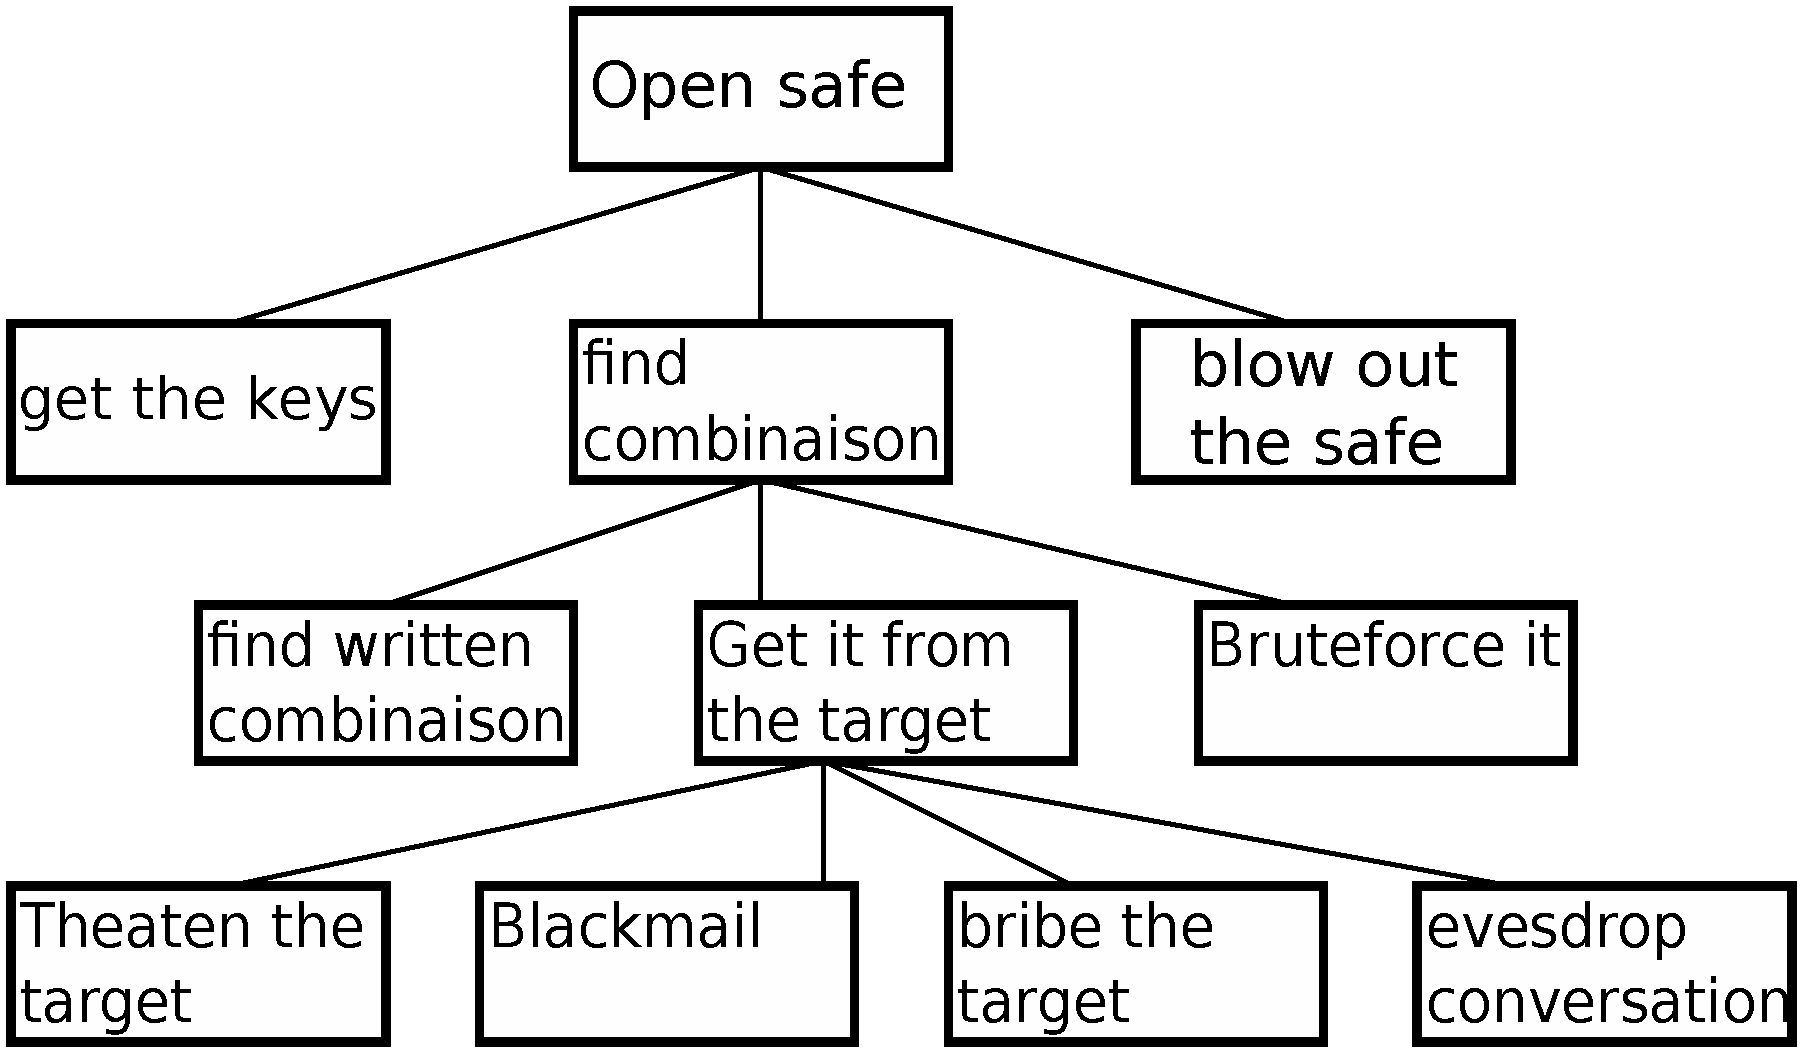
\includegraphics[width=0.55\textwidth]{schema/attack_tree.pdf}
    \caption{Attack Tree example}
    \label{attack}
\end{figure}

Attack tree is a 3-tuple $AT = \{N, C, L\}$ where :

\begin{itemize}

\item $N$ is the set of all the existing nodes with their name.

\item $C$ are the connections between nodes, it describe how each nodes
  are connected to each other like this $\{node_1; node_4; node_9\} \rightarrow
  node_5$

\item $L$ represent all the label that can be attributes to a node.

\end{itemize}

\subsection{Fault tree}

Fault trees in contrary of attack tree is used to represent safety
fault that can occurs inside a system, and to check the different
consequences those errors can lead to. They are represent as a tree
where all node are connected to each other with logical gates. So this
representation is done with DAG, that have two types of nodes, \emph{event}
and \emph{logical gates}An example fault tree is shown in the figure
\ref{fault}\newline
An \emph{event}node represent a failure that can occur in the system or
the failure of a component. Those event are divided into basic event
(BE) that occur spontaneously, and intermediate event (IE) that are
caused by other event. The event at the top of the tree is call the
top event (TE) and is the one that is analyse inside the fault tree.

\begin{figure}[h]
    \centering
	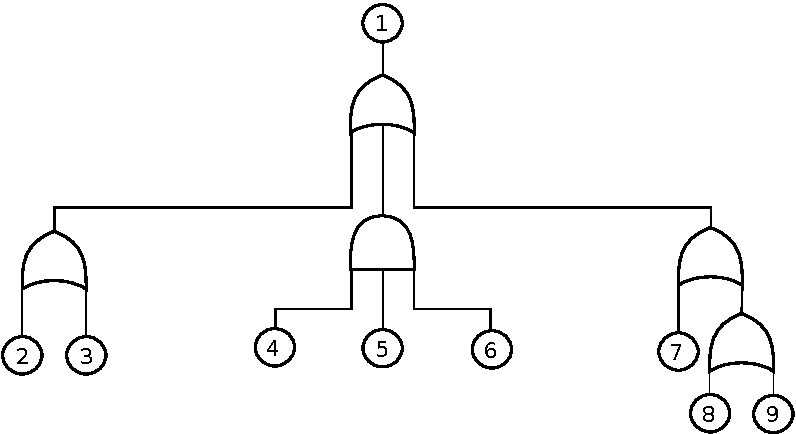
\includegraphics[width=0.5\textwidth]{schema/fault_tree.pdf}
    \caption{Fault Tree example}
    \label{fault}
\end{figure}


Fault tree is a 4-tuple $FT = \{E, G, T, C\}$ where :

\begin{itemize}

\item $E$ represent the set of all the existing event of the tree.
  
\item $G$ represent the set of all gates that exist on the tree.
  
\item $T$ represent the type each gate can take.

\item $C$ represent the connection between gate and events.

\end{itemize}
    
\subsection {(Dynamic) Reliability Block Diagrams (D)RBD}

\subsubsection{Reliability Block Diagrams}

Block diagrams are a way to represent a system by using blocks. Each
component of the system is represented as a block connected, either
directly or in parallel. An example of RBD is shown in Figure
\ref{RDB}. \newline
Each of these blocks is subdivided into smaller blocks that represent
the behavior of the component. Each block contains a failure rate
associated with it. \newline
An RBD can be represented as a logical formula in which the blocks in
series are connected by \emph{and}and the blocks in parallels by \emph{or}.

\begin{figure}[h]
    \centering
	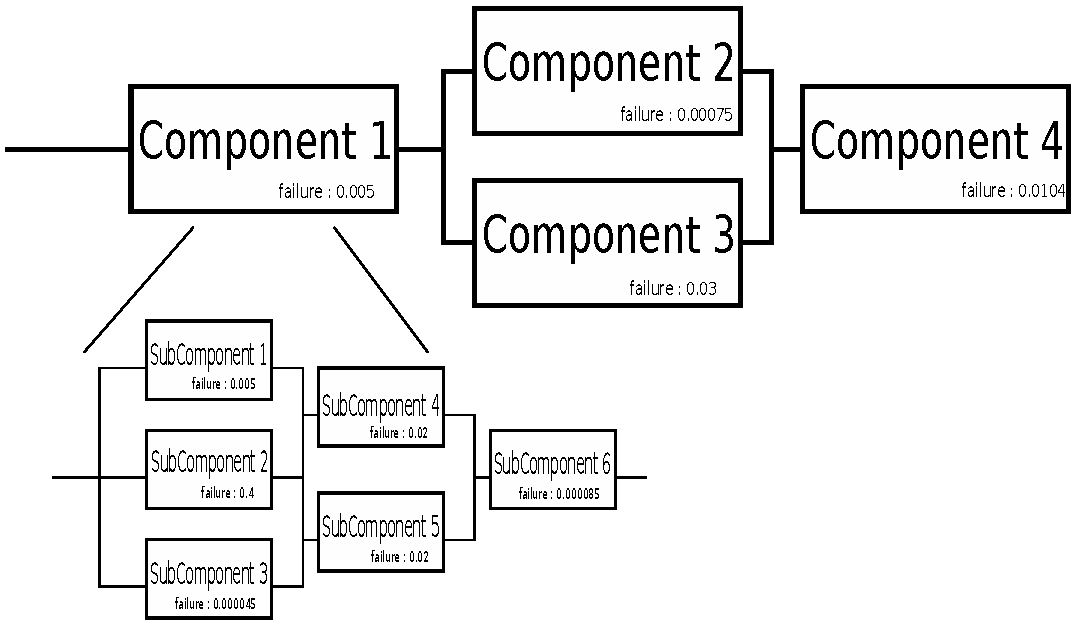
\includegraphics[width=0.65\textwidth]{schema/RDB.pdf}
    \caption{Reliability Block Diagram example}
    \label{RDB}
\end{figure}

Each block is represent like this $B_i\{L\}$ where $_i$ represent the
identifier of the block and $L$ the probability of failure associated
to this block.

Each block can be decompose into a block diagram so as example $B_i =
B_{j} \wedge (B_{k} \vee B_{l}) \wedge B_{m}$

So a RBD is represent by a succession of Block link with each other by
$and$ and $or$ gates.


\subsubsection{Dynamic Reliability Block Diagrams}

Dynamic Reliability Block Diagrams are static ones in which some new
\emph{special}block have been added to make the behaviour of the system it
represents dynamic. Those blocks are SDEP (State Dependency) block,
Spare block, LSH (Load Sharing) block, SEQ (Sequential) block and PAND
(priority) block. \newline

\textbf{SDEP block}are used to model the dependency between multiple
state. Each state affect to it can send and receive 3 type of signal
from this block. $A$ for \emph{Active}, $D$ for \emph{Deactivation} and $F$ for
\emph{Failure}It is used to have a reaction or dependency between
state. If one become activate, one other can be deactivate. By the
same way it is possible to represent the reaction to a system if one
component fails. This is shown in figure \ref{sdep}.

\begin{figure}[h]
    \centering
	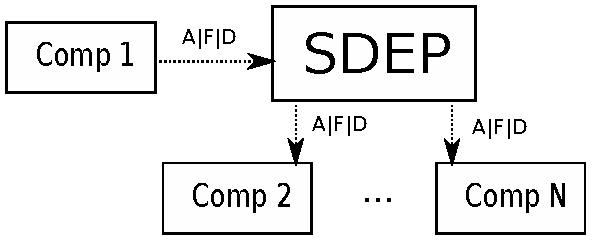
\includegraphics[width=0.35\textwidth]{schema/sdep.pdf}
    \caption{SDEP Block example}
    \label{sdep}
\end{figure}


\textbf{Spare block}are here to model the behaviour of the redundant
component. The primary component can send a $D$ or $F$ signal to the
Spare block that will send $A$ signal to different subcomponent. So
the order of usage the redundant component can be modelize. This is
shown in figure \ref{spare}.

\begin{figure}[h]
    \centering
	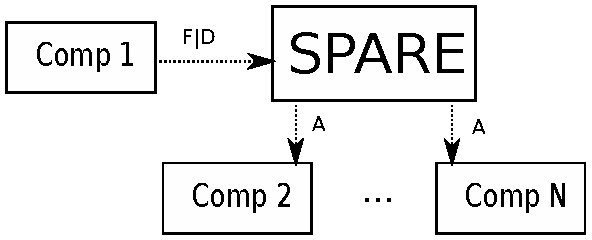
\includegraphics[width=0.35\textwidth]{schema/spare.pdf}
    \caption{Spare Block example}
    \label{spare}
\end{figure}


\textbf{LSH block}are here to help to share the load over the multiple
component. This block get two variable $k$ and $n$ which represent
respectively the minimum number of active component connect to it, and
the total number of component connect to it. So if there is k active
component connect to this block and one become deactivated or fail,
then this block will send a $D$ signal to every other component
connect to it. This is shown in figure \ref{lsh}.

\begin{figure}[h]
    \centering
	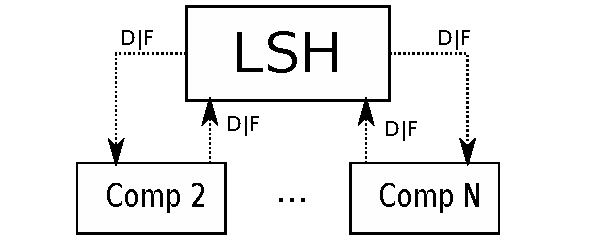
\includegraphics[width=0.35\textwidth]{schema/lsh.pdf}
    \caption{LSH Block example}
    \label{lsh}
\end{figure}


\textbf{SEQ block}are used to specify the order in which some event can
happened between the component connect to it. So it is possible to say
that \emph{component 1}must fail before \emph{component 2}can fail too. In
other way, the \emph{component 2}can't fail before \emph{component 1}fails.

\textbf{PAND block}are used to modelize the occurrence order of some
components. It can be used for this kind of example : If a primary
component is connect to a switch controller as well as a redundant
component. If the primary component fail and the switch is still alive
the redundant component can be activated, but if the primary component
and the switch failed, the redundant component can not be activate and
the system fails.

All those new blocks are used to make the behaviour of a RBD system
dynamic. An example system is shown in figure \ref{DRBD}

\begin{figure}[h]
    \centering
	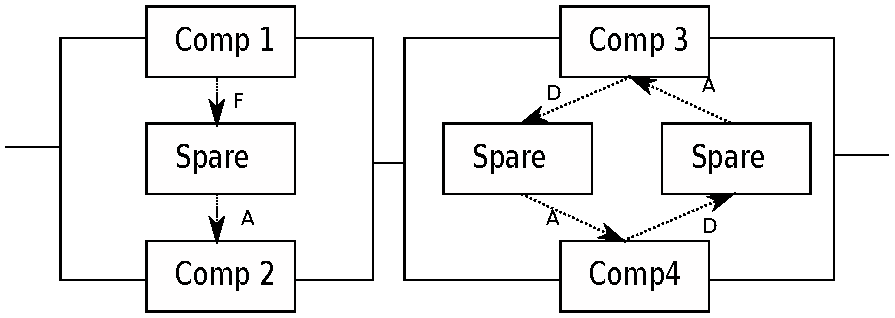
\includegraphics[width=0.65\textwidth]{schema/drbd.pdf}
    \caption{Dynamic Reliability Block Diagram example}
    \label{DRBD}
\end{figure}

\subsection{Boolean logic Driven Markov Processes (BDMP)}

Boolean logic Driven Markov Processes are here to help make fault tree
more dynamic by the addition of Trigger Markov Process. So the basic
concept of it is that every leaf of the fault tree does not represent
any more some basic fault event that could occurs but a Trigger Markov
Process. One Example of a BDMP is shown in figure \ref{bdmp}.

\begin{figure}[h]
    \centering
	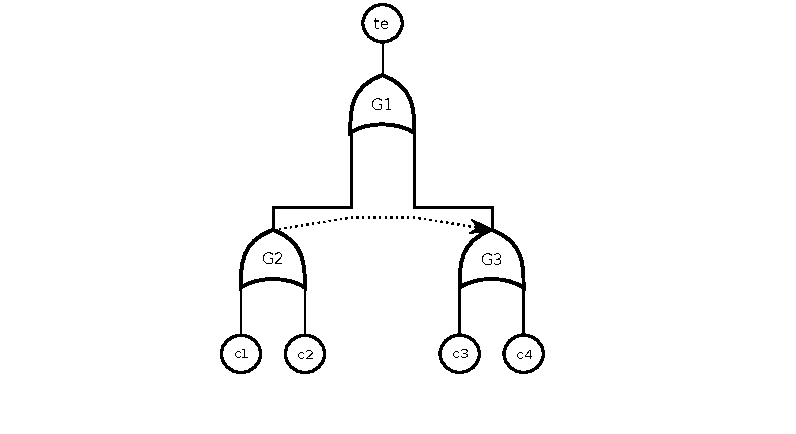
\includegraphics[width=0.75\textwidth]{schema/BDMP.pdf}
    \caption{BDMP example}
    \label{bdmp}
\end{figure}


So Each TMP are composed of four states, Standby, Faulty during
Standby, Working and Faulty during Working, and gets two boolean
variable \emph{Activation Status} and Failure Status. One example can be
seen if figure \ref{tmp}. \newline
So those four states models 2 Markov Chain, one for the behaviour of
the Working state of the component and one for the behaviour of the
standby state of the component. It is possible to  go from one to the
other. \newline
The trigger event represent with a dash line from G2 to G3 leans that
when the output of G2 is True the part the of the system related to
G3, c3 c4, are required. And is the output is False then they are not
required.

\newpage

\begin{figure}[h]
    \centering
	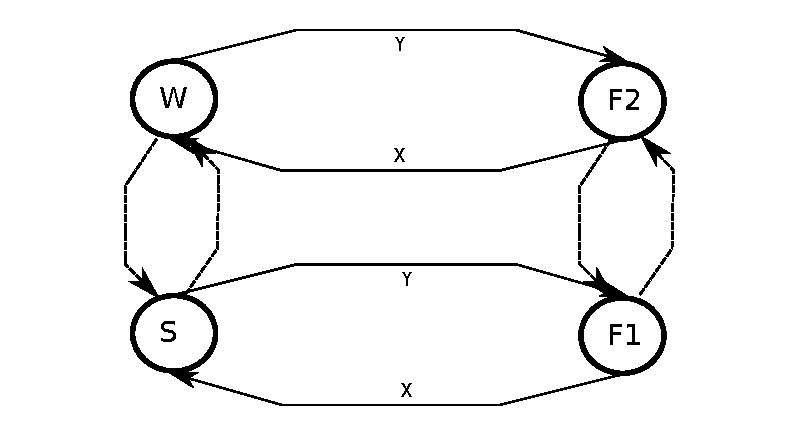
\includegraphics[width=0.5\textwidth]{schema/TMP.pdf}
    \caption{TMp example}
    \label{tmp}
\end{figure}


\subsubsection{Boolean logic Driven Markov Processes formalism}

Boolean logic Driven Markov Processes are a 3-tuple $BDMP = \{FT, TMP, Tr\}$ where :

\begin{itemize}

\item $FT$ represent the Fault Three.

\item $TMP$ represent the set of all TMP associated to each leaf of the fault tree.

\item $Tr$ represent the set of triggers

\item $te$ represent the top-event of the fault three

\end{itemize}

\subsection{CVSS}


\textbf{Common Vulnerability Scoring System}(CVSS) as describe in its Specification
Document ~\cite{CVSS} is a way to score the vulnerability of our system
over an online calculator. After completing to enter the entries in
the calculator, we get a score between 0.0 and 10.0. It can be a good
start to see how much the system can be vulnerable. \newline
They says that this tools gives us three good things :

1) A standardized vulnerability scores.
2) an open framework, so we can see how the score is compute.
3) get a vulnerability risk order.

They separate the data in 3 metrics, base group, temporal group and
environmental group. \newline 
The base group is cut in half, there is the exploitability that refers
to all the vulnerable things and the impact that refers to the
consequence of a break in the system. \newline
The temporal group is about all the characteristics that could get
more vulnerable over time but not in the environment. Like if it
already exist a kit to exploit the known vulnerabilities or if they
got to create one. \newline
And the environmental group refers to all the environment
vulnerabilities of the system.

\newpage

\section {Network}

\subsection {Multipath TCP}

\label{sec:mptcp}

{\Huge M}ultiPath TCP *(MPTCP)* is a derivative of the TCP protocol, both
being used to implement communications between two objects. The
purpose of MPTCP was initially to improve the connecticvity between
two objects on the network by defining several possible routes between
them. Therefore, if one of the routes is not working properly, packets
can still be transmitted using one of the other routes.

MPTCP was first specified in 2013 and updated in 2019, and is
available on most existing platforms (\emph{i.e.} Linux kernel, FREE
BSD, IOS, MAC OS, etc.). Nowadays, MPTCP is mainly used in mobile
networks, as it allows a mobile device to use both its Wi-Fi and
cellular network interfaces to communicate with services: the
interface connected to the least congested route will be used.

In a MPTCP configuration, it is possible to declare the set of
interfaces through which an object can communicate, as well as the
priority associated with each interface.  This allows a system to keep
the TCP connection open, even when one of these interfaces no longer
works.

In our work, we propose to use MPTCP and its capacity to define
multiple routes, as a way to maintain connections among objects while
being able to redefine their communication routes. We also propose to
use the IPv6 communication protocol for connections with services on
the Internet. We explain the reasons of this choice in next
subsection.


\subsection {IP v6}

\label{sec:ipv6}

IPv6 is the successor of IPv4, even though the latter one is still
massively used by many existing systems. However, the number of
available addesses on IPv4 networks is limited: being encoded with
\emph{32 bits}, approximately $4.3*10{9}$ addresses are available on an 
IPv4 network. On the other hand, IPv6 addresses are encoded with
\emph{128 bits}, leading to approximately $3.4*10^{38}$ available
addresses.

An IPv6 network is divided into subnetworks identified in IPv6 addresses by a
prefix of size varying from 1 to 64 bits. The remaining bits are then used to
identify a host on this subnetwork. Assuming a subnetwork is identified with 64
bits -- which is the smallest possible subnetwork -- these host identifiers
are then encoded with 64 bits. The number of available addresses to identify
hosts in this subnetwork is approximately $1.84*10^{19}$.
These numbers are required to compute the time an attacker would need
to identify the IP address of an object connected to a given
subnetwork. 

In the remainder of this subsection, we describe how IPv6 addresses
can be assigned to objects: automatically, manually and managed by a
DHCP server.

An automatic address assignment may cause security problems since IPv6
addresses are derived from the interface MAC address, and each MAC
address is unique. This allows an attacker to probe the exchanges from
a particular host and track its communications. This is problematic
in the context of connected objects: using automatic assignment, IP
addresses of connected objects would not change over their
lifetime. Therefore, a vulnerable object can be retreived very easily
by an attacker who already identified it.

A manual assignment of IPv6 addresses consists in letting objects
determine their own IP address. As a consequence, it is under the
responsibility of the object provider to define mechanisms preventing
attackers to track this object on the network. This also poses a
network management problem since address assignment is decentralized,
which can result in address collisions.

The last possibility is to assign IP addresses to objects using a DHCP (\emph{Dynamic Host Configuration Protocol})
server. This allows to assign or reassign addresses to objects
without collisions by using the routing table of the DHCP server. The
address assigned to an object is no longer derived from its interface
MAC address, making it more difficult to track. However, this poses
another problem: the DHCP server must be well secured in order not to
allow access to the different data it contains. This problem is out of
the scope of this paper, and could also take advantage of deploying
MTD mechanisms on the DHCP server.


\subsection {Car Network Topology}

The hosts of the network we consider in this paper are cars seeking
to connect to the Internet in order to have access to different
services, such as navigation or entertainment services as well as
traffic information. Traffic information may be provided by other cars
and infrastucture objects located on the road (\emph{e.g.} signs,
lights or traffic lights).

In order for these different devices to communicate with each other,
they must be assigned IP addresses, which will be done by a DHCP
server. For the sake of simplicity, we assume each car manufacturer
holds an IPv6 subnetwork to which cars produced by this manufacturer
are connected. Of course, other options are possible, for instance car
manufacturers could rent and share a network provided by a thrid
party.

The manufacturer's subnetwork is accessible all over the world, and
all the connected cars of its brand are connected to it. The
subnetwork's DHCP server is used to assign IP addresses to all the
cars, and manage the addresses consistency in order to avoid addresses
collisions during addresses (re)assignment. This DHCP server is also
used to route the different messages on the subnetwork.

The subnetwork topology described hereabove is depicted on figure
\ref{netw}: the DHCP server links the cars connected to its subnetwork
to the Internet. All the cars of a given manufacturer are connected to
the same IPv6 subnetwork, managed by this DHCP server. All the
messages circulating on the subnetwork are transmitted to the DHCP
server which routes them to the recipient car.

\begin{figure}[h]
    \centering
	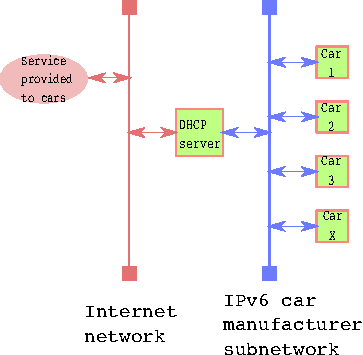
\includegraphics[width=0.45\textwidth]{schema/net_topo.pdf}
    \caption{Network Topology Representation }
    \label{netw}
\end{figure}


Given this topolgy, cars connection is performed as follows. Each time
a car is started, it tries to connect to the internet by broadcasting
a message to the entire subnetwork. This message is a request for an
IP address, and should be treated by the DHCP server. This is followed
by a series of message exchanges until the DHCP server assigns to this
car an IPv6 address. Note that these various messages are sent in
plain text and readable by any object connected to the subnetwork and
listening to it. Of course, this raises security issues since attacker
can easily know the IP address of hosts: the IP addresses assigned
initially have to be modified.

In addition a host receiving an IP address from a DHCP server receives
at the same time a lease time for this address: the host will have to
request a new address to the DHCP server before the end of its
lease. As these messages are also sent in plain text on the network,
it makes it easy for an attacker to track address changes of a car.


\subsection {Attack Entrypoints}

Attackers may attempt to comprize a car from outside the subnetwork
the car is connected to (i.e. from a system connected to the Internet
from outside the subnetwork), or from the inside of this subnetwork
(i.e. from a system already present on the subnetwork). In each case,
the attacker's method will be different since he or she does not have
access to the same information and resources.

An attacker located outside the subnetwork cannot easily read the
various messages circulating on that subnetwork. He or she then must
scan the different subnetwork addresses in order to find a system
connected to this subnetwork. Once found, he or she will then need to
retrieve informations about the car system he or she found before to
launch his or her attack. It must ensured that defense methods
deployed in connected cars allow these cars to hide from an attacker
scanning their subnetwork from the outside (\emph{e.g.} from the
Internet).

An attacker located inside the subnetwork can see the messages
circulating on the network. Even though the payload of these messages
can be encrypted, the address of the sender and receiver of each
message circulates in plain text. An attacker located inside the
subnetwork can thus see the IP address of cars connected to this
subnetwork by listing to the circulating messages. Therefore he or she
does not need to scan the subnetwork to find IP addresses of connected
cars. We must then ensure that defense methods deployed in connected
cars allow these cars to escape from an attacker trying to attack from
within the subnetwork.

It is therefore necessary that the defense methods we propose in this
paper allow a car connected to a subnetwork to *both hide* from an
attacker outside the subnetwork, \emph{as well as to escape} from an
attacker connected to this subnetwork.

This problem is very significant in the context of connected cars,
because attacks may propagate from inside the subnetwork itself. This
is one of the reasons why the attack against the Jeep \cite{Jeep} became
so popular: after taking control of the car scientists had physical
access to, they demonstrated their capacity to take control over other
cars remotely.


\subsection {Time to find An IP}


\label{sec:soa}

Consider a car manufacturer that produces on average 6 millions cars
per year. If these cars have a 20-years lifespan, and all of them are
connected at the same time to the network, the maximum number of hosts
is 120 millions. This is way bellow the number of addresses that can
be encoded for hosts using IPv6, even when considering subnetworks
identified with 64 bits in the IP address.

In order to consider the worst-case, we assume all the cars of the
manufacturer are actually used at a given time, \emph{i.e.}
$120*10^6$. We want to estimate how long it would take for an attacker
outside the subnetwork to reach a 50\% probability to find the IP
address of one car on this subnetwork. We assume a subnetwork
identified by a 64 bits prefix, which is also a worst-case hypothesis:
it minimizes the possible number of identifiers for hosts. Still, the
number of possible identifiers is huge: $2^{64}$, \emph{i.e.}
approximately $1.85*10^{19}$.

For estimating the time an attacker needs to scan the network, we
consider a well-known open source tool for scanning networks: *nmap*. In
fact, *nmap* can be used to discover hosts and services on a network by
sending packets and analyzing the responses. *Nmap* can also provide
further information on targets (\emph{e.g.} reverse DNS names, device
types, *MAC* addresses, etc.). Using *nmap* with highly optimized options,
the time needed to scan one IP address is approximatly 255 ms
\cite{nmap_2009}. 

Now that we have all the inputs to compute the time needed for an
attacker to reach $50\%$ probability to find the IP address of
a car, here is how the computation works. We apply the *urn
statistical model* \cite{carroll_2014}, to solve the problem of \emph{Drawing
With Replacement}. This means we consider the attacker randomly scans
the network until he or she finds a host, and the same address can be
scanne more than once.

The mathematical formulation of this problem is given by equation
\eqref{one}, where $x$ is the number of attempts, $h$ is the
number of hosts on the network, $a$ is the number of available
addresses on the subnetwork and $Proba$ is the percentage of
probability to find an objects over the network.

\begin{equation}
Proba = 1 - (((a-h)/a)^x)
\label{one}
\end{equation}

For an attacker outside a subnetwork identified with a prefix of 64
bits in IP addresses (\emph{i.e.} $a=1.85*10^{19}$), the time to reach
$Proba=50\%$ chance of finding the IP address of a vehicle among
$h=120*10^6$ million vehicles, considering 255 ms to scan an IP
address, is $3 \cdot 10^{13}$ s, or approximately 951 years.


\section {Cyber-security principles}
\medskip
{\Huge C}yber-security is build on 3 pillars; the CIA triad.


The security goal is to provide safetymeasures to achieve the confidentiality, integrity, and availability (CIA) triad for protection of the overall system along with its peripherals. The triad CIA is as follows:
\begin{itemize}
    \setlength\itemsep{1em}
    \item \emph{Confidentiality}: The aim of confidentiality is to protect the critical information from unauthorized users. Confidentiality for network security ensures that the critical assets are accessible only to authorize users.
    \item \emph{Integrity}: This ensures that unauthorized users do not modify or manipulate the data or information during their network transmission.
    \item \emph{Availability}: The availability is the last component of the CIA triad that represents the real availability of our information. Authentication methods, channel access, and systems all have to function efficiently to prevent the data and make sure that it is available when required. In short, the availability aims to ensure that data and network resources are available when requested by the authorized users.    
\end{itemize}

%% \FloatBarrier
%% \begin{figure}[ht]
%% 	\centering
%%     \includegraphics[scale=1.0]{CIA-triad}
%%     \caption{3 pillars of the security}
%%     \label{fig:CIA}
%% \end{figure}
%% \FloatBarrier

Besides the CIA triad, Identification, Authentication, Authorization, Auditing and Accounting (called AAAA) also play an important role for controlling the access to the system resources. The AAAA is a term for controlling the access to the system resources, auditing usage, enforcing policies, and offering the details need to charge for services.
\begin{itemize}
    \setlength\itemsep{1em}
    \item \emph{Identification}: Identification aims of claiming to be an identity when attempting to access a resource. Providing an identity can involve typing or sending a username or an ID, swiping a smart card, waving a proximity device $\ldots$. Without an identity the system has no way to correlate an authentication factor to the subject. 
    \item \emph{Authentication}: Authentication is about proving that you are that claimed identity. It requires the subject to provide additional information that correspond to the identity that is claimed. The most common form is to provide a password. Authentication verifies the identity of the subject by comparing one or more factors against the database of valid identities.
    \item \emph{Authorization}: Authorization is defining the permissions of a resource/object access for a specific identity. It ensures that the access to a resource/object is given the right and privileges assigned to the authenticated identity. If the requested action is allowed, the subject is authorized, instead the subject is denied. It is not because a subject is correctly authenticated that he/she has the right to perform any actions on any resource.
    \item \emph{Auditing}: Auditing is recording a log of events and activities related to the system, subjects and objects. It purposes to track and record all subject requests and actions. Log files provide an audit trail for re-creating the history of events. It permits to detect malicious actions, system failures but also system performances
    \item \emph{Accounting}: Accountability aims to reviewing the log files to check for compliance or violation of security policy in order to hold the subject accountable of his/her/its actions. It is also a way of evaluating what services have been used and how many resources have been consumed.
\end{itemize}


Les principales techniques utilis\'ees pour garantir ces 3 propri\'et\'es sont:
\begin{itemize}
\setlength\itemsep{1em}
\item \emph{Chiffrement (Encryption)}: La transformation de l'informations originale (appel\'e clair) \`a l'aide d'une cl\'e de chiffrement, de telle sorte que les informations transform\'ees (appel\'e chiffr\'e) ne puissent \^etre interpr\'et\'ees que par un autre utilisateur ayant connaissance de la cl\'e de d\'echiffrement (qui peut, dans certains cas, \^etre identique \`a la cl\'e de chiffrement). Pour \^etre en s\'ecurit\'e, un algorithme de chiffrement doit rendre extr\^emement difficile pour quelqu'un de d\'eterminer tout ou partie des informations clairs sans connaissance de la cl\'e de d\'echiffrement ou faiblesse de l'algorithme de chiffrement. 

\item \emph{Authentification (Authentication)}: La d\'etermination de l'identit\'e qu'un sujet (personne, logiciel ou \'equipement). Cette d\'etermination peut \^etre effectu\'ee par plusieurs moyens. Il est g\'en\'eralement bas\'e sur une combinaison de quelque chose que la personne conna\^it (Something you know) comme un mot de passe ou un code PIN, quelque chose le sujet poss\`ede (Something you have) comme une carte \`a puce contenant des cl\'es secr\`etes un t\'el\'ephone pour recevoir un code, un passeport, ou quelque chose la personne est (Something you are) comme une empreinte digitale.

\item \emph{Contr\^oles d'acc\`es (Access Control)}: Ensemble de r\`egles et politiques de s\'ecurit\'e qui limitent l'acc\`es aux informations aux sujets (personnes et/ou syst\`emes) ayant un \emph{besoin d'en connaitre}. Ce besoin d'en connaitre est d\'etermin\'e suite \`a l'authentification correcte du sujet, de par son identit\'e ou r\^ole. Un ensemble de r\`egles est pr\'e-d\'efinie par le gestionnaire de la s\'ecurit\'e informatique en se basant sur la politique de s\'ecurit\'e.

\item \emph{Signature (Signature)}: La signature d'une information a deux objectifs; assurer que l'information sign\'ee n'a pas \'et\'e alt\'er\'ee depuis la signature et authentifier la source de l'information (non-repudiation). La signature consiste en un chiffre d\'ependant d'une cl\'e secr\`ete connue uniquement par le sujet signant l'information et du contenu du message \`a signer. Une signature est v\'erifiable, sans connaitre la cl\'e secr\`ete, par une partie tierce en cas de litige entre parties. Si le contenu du message ou la signature est modifi\'e, la correspondance entre le contenu initial et message et sa signature sera invalide permettant de d\'etecter l'alt\'eration et de rejecter l'information. De fa\c con, sym\'etrique, si le contenu du message et sa signature correspondent alors la source de l'information ne pourra pas nier avoir sign\'e l'information car elle est la seule \`a connaitre la cl\'e secr\`ete.

\item \emph{Responsabilit\'e (Accountability)}: La capacit\'e de rendre le sujet responsable de ces actions. Ceci est r\'ealis\'e en s'appuyant sur des journaux d'audit (audit log). Une fois le sujet correctement authentifi\'e, toutes ces actions sont enregistr\'ees sous forme d'\'ev\'enements dans un journal d'audit. En cas d'investigation ou de fa\c con p\'eriodique, le gestionnaire de la s\'ecurit\'e informatique peut r\'ealiser un audit des journaux pour identifier la source potentielle d'une attaque.

\item \emph{Sensibilisation \`a la s\'ecurit\'e (Security awareness)}: La principale source de risque pour une organisation ne provient pas de faiblesse dans la technologie des \'equipements mais d'actions (ou d'inaction) de la part des utilisateurs du syst\`eme. Afin de limiter ce risque, il est n\'ecessaire de former les utilisateur aux diif\'erents risques informatiques et aux bonnes pratiques pour assurer le niveau de s\'ecurit\'e requis. 

\item \emph{S\'ecurit\'e physique (physical security)}: Mise en place de barri\`eres physiques pour limiter l'acc\`es aux ressources sensibles. Ces barrières comprennent sont mutiples comme le gardiennage, la vid\'eo-surveillance, les serrures sur les armoires et les portes, les chambres fortes, l'utilisation de matériaux insonorisants, ou m\^eme la construction d'\'equipement renforc\'e (tempest) afin que les signaux \'electromagn\'etiques ne puissent pas entrer ou sortir.

\item \emph{Tol\'erance aux fautes (fault tolerance)}: Ensemble de techniques peuvent \^etre utilis\'ees pour garantir le syst\'eme en op\'eration.
\end{itemize}


\FloatBarrier
\begin{table}[ht]
\centering
\begin{tabular}{| l | c | c | c |}
\hline
& Confidentialit\'e & Integrit\'e & Disponibilit\'e \\
\hline
Chiffrement & \checkmark & &  \\
\hline
Authentification & \checkmark & \checkmark &  \\
\hline
Contr\^oles d'acc\`es & \checkmark & \checkmark &  \\
\hline
Signature &  & \checkmark &  \\
\hline
Responsabilit\'e & \checkmark & \checkmark &  \\
\hline
Sensibilisation \`a la s\'ecurit\'e physique & \checkmark & \checkmark & \checkmark \\
\hline
S\'ecurit\'e physique & \checkmark & \checkmark & \checkmark \\
\hline
Tol\'erance aux fautes & & & \checkmark \\
\hline
\end{tabular}
\caption{Principales m\'ethodes de la s\'ecurit\'e informatique}
\label{tab:cia}
\end{table}
\FloatBarrier


Dans le reste de la th\`ese, nous concentrerons sur la disponibilit\'e des syst\`emes embarqu\'es. 












\chapter{Connected Cars} \label{CARS}
\smallskip
\hfill
\begin{minipage}[b]{8cm}
%{\it This work was presented in part at the conference of one-legged deaf-mutes in Quiberon in April 1994.}
\end{minipage}
%\begin{flushright} Remoi \end{flushright}
\vskip 2cm


\section {The software revolution}
\medskip
{\Huge E}mbedded software is one of the key innovation in the automotive world. From the paper of
 Robert Charette (\cite{Cha2009}) published in IEEE Spectrum, the first car embedding a software was the Oldsmobile Toronado from General Motors in 1977. The Toronado enclosed an \gls{ecu}\@ which managed the spark timing. In 1978, General Motors offered on the Cadillac Seville as an option a trip computer able to display the speed, the fuel level, trip and engine information. This product was based on an embedded version of a Motorola 6802 and had about 50,000 lines of code. Since, more and more functions are performed by software in a car. To limit the volume of cable in a car, all the sensors and on-board unit are now connected to a network backbone using CAN or xxx network. As the computing power of the processor grows, new functions appear in cars. Cars become now on-wheel software platform like airplanes or trains.A modern family car embeds between 30 and 50 ECUs performing the management of the multiple systems(see \ref{tab:soft}). A premium car can have up to 3,000 singular functions performed by software.   

\FloatBarrier
\begin{table}
\centering
\begin{tabular}{| l | l | l |}
\hline
Airbag & ABS & Anti-thief system \\
\hline
Air Conditioning & Speed control & motor management \\
\hline
Turn signals & Headlights & Klaxon \\
\hline
Seat management & Navigation system & Audio system\\
\hline
Wheel pressure & management of the doors and windows & ... \\
\hline
\end{tabular}
\caption{Software function in a car}
\label{tab:soft}
\end{table}
\FloatBarrier


In 2009, Alfred Katzenbach, Director of Information Technology Management at Daimler announced that the radio and navigation management system of an S-class Mercedes-Benz contains over 20 millions line of code and the car embeds nearly as many ECUs as an Airbus A380 (excluding the in-flight entertainment system) (\cite{Cha2009}). Software in a car has an exponential growth in size and complexity. In just 10 years, the software volume in a car expands by a factor 10, to arrive at around 150 million of lines of code. A model S from Tesla is equipped with a 17' tactical display based on a Linux kernel which controls almost every driver functions. In fact, there is only 2 manual buttons that are not management by software in the car, the blinker and the glove's compartment.


A side effect of this revolution is the complexity and the richness of the functions proposed to the driver. It is frequent to have the driver manual of a car with over 500 pages to explain all the driver functions. Automotive experts estimate that an average driver uses not more than 20\% of those functions. Thus is why, some automotive manufacturers are asking them the question of a limitation (or reduction) of software functions proposed in a car. For example, is it really necessary to have the ceiling light of a car going out gradually when the doors are closing?\\

The growth of the software in a car has also important consequences on the way to maintain and repair a car. An estimation gives that more than 50\% of the ECU that are changed by a car mechanic have no software or hardware failure. Mechanic frequently replaces pieces without the knowledge of the root cause of the issue. Now, one of the most frequent activity of a car mechanic is to download and upgrade new version of software. Some car manufacturer, like Tesla proposes to download software updates, including software corrections (patches) or new functionalities, using the cellular network without any involvement of a car mechanic.


Today, the cost of the software and the supporting electronic in a car is estimated between 35\% and 40\% of the cost of a car. Investment to develop new software platform became so expensive that the main European Automotive manufacturers develop a series of standards to reduce the developent cost:
\begin{itemize}
    \item a commom platform; \emph{Automotive Open System Architecture (AUTOSAR)} \cite{AUTOSAR} allowing there suppliers to develop a single platform interoperable between several manufacturers. 
    \item a software development framework for the safety; \emph{Road vehicles, Functional Safety package} ISO 26262 \cite{ISO26262}
    \item and recently a standard to address the cybersecurity management system; \emph{Road vehicles - Cybersecurity engineering} ISO 21434 \cite{ISO21434}.
\end{itemize}

Introduction of software in the car permits to have safer and less polluting cars but it has open the door at two new risks the \emph{software safety risk} and the \emph{cyber-security threat}. 

\section {Modern car software architecture}

\subsection {AUTOSAR}

\gls{autosar}\@ was founded in 2003, with the goal to develop an architecture, independent of the underlying ECU hardware that the automotive industry can use to reduce the increasing complexity of software in modern vehicles (\cite{AUTOSAR}). This is the de facto standard for the automotive software today. AUTOSAR makes an abstract layer of the underlying hardware, so that the applications written on top of AUTOSAR are independent from the actual supplier of the ECU hardware. The AUTOSAR standard documentation guides companies and the automotive industry in designing and implementing software in their vehicles. Besides the Software architecture and the Standardized \gls{api}\@, AUTOSAR provides a Software development methodology. By adopting the AUTOSAR standard, companies can develop software solutions that are independent of the hardware they are running on, and this software can run on any ECU in the vehicle. 
\bigskip

AUTOSAR is a three-layered architecture (\cite{AUTOSAR_archi}): 
\begin{itemize}
    \item the \emph{application layer} provided by the software company implementing the specific functions of the ECU. This is the highest layer which contains the software components (SWCs). AUTOSAR application (e.g., ABS, Cruise Control $\ldots$) consists of several SWCs, which provide the core functions. An AUTOSAR SWC is an atomic piece of software that cannot be divided and is located a single ECU. 
    \item the \emph{run-time environment (RTE) layer}. The RTE layer provides the standardized interface between the SWCs and the basic software layer. Because of this layer, SWCs can be used on different ECUs, independent of the ECU vendor.
    \item the \emph{basic software (BSW) layer} that consists of four sub-layers; the \emph{services layer} providing operating system functions like communication services, memory services, diagnostic services, $\ldots$. The layer also contains the main security mechanisms. The \emph{ECU abstraction layer} makes higher software layers independent of ECU hardware layout. It provides an application programming interface to devices regardless of their location (internal/external of the microcontroller). The \emph{Microcontroller abstraction layer}. It contains drivers for direct access to the upderlying microcontroller and internal parameters. It makes higher layers independent of the microcontroller. The \emph{complex drivers layer} which provides the ability to integrate special-purpose functions such as drivers for devices that are not specified with the AUTOSAR standard. This layer accesses directly the microcontroller. 
\end{itemize}

Each of the sublayers offers different services as shown in \ref{fig:AUTOSAR_archi}. 

\FloatBarrier
\begin{figure}
    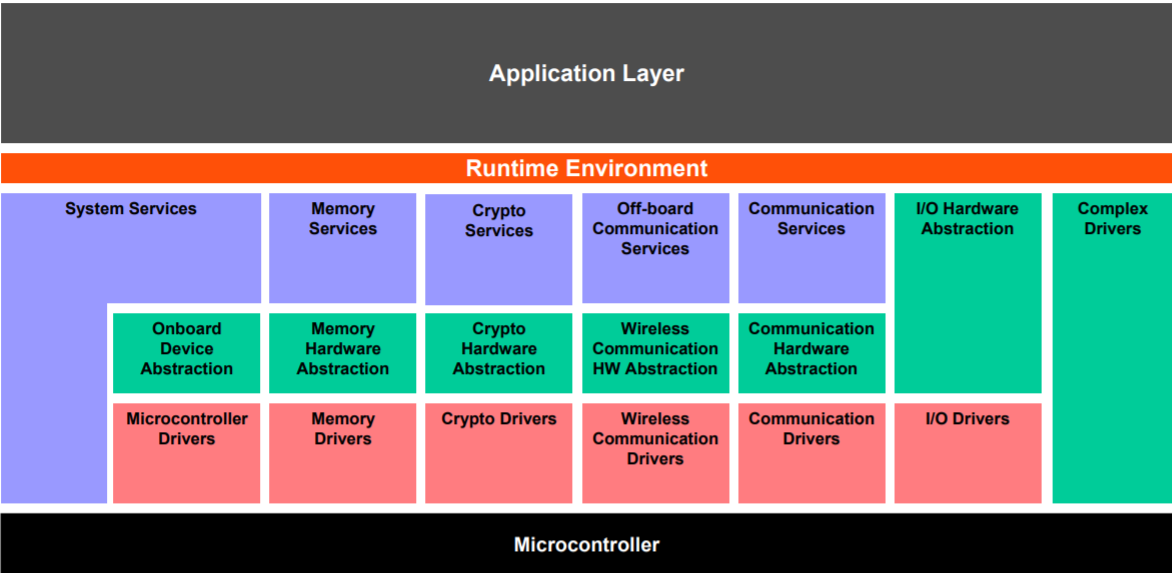
\includegraphics[width=\textwidth]{AUTOSAR_architecture}
    \caption{AUTOSAR layered architecture}
    \label{fig:AUTOSAR_archi}
\end{figure}
\FloatBarrier

The AUTOSAR standard defines security mechanisms that can be used by the software modules implemented into the vehicle system. It further specifies interfaces and procedures to provide Secure On-Board Communication, and the exact implementation is left for the OEMs to decide on. OEMs choose the cryptographic algorithms and encryption techniques which they want to implement and use in the vehicle system.


AUTOSAR has been mainly build to ensure a high level of Safety of the system. Many safety mitigations requested by the standard can be attack vectors. For example (see \cite{Nas2017}), to protect the internal and external communication, AUTOSAR defines the \Gls{ete}\@ library which defines the safety mitigations to prevent safety critical functions from operating on faulty or missing data. The mitigations are:
\begin{itemize}
    \item \Gls{crc} check to detect corruption of data
    \item Sequence counter to detect out of sequence messages and to osrt the messages
    \item Alive counter to prevent operating on old data
    \item A unique ID for Interaction Layer Protocol Data Unit (I-PDU) group to detect a fault of sending I-PDU on unintended message
    \item Timeout monitoring to detect communication loss with the sender.
\end{itemize}

Attack based on those mitigations will lead to a rejection of the messages and a potential \Gls{dos}\@. No mechanism has been provided to detect the difference betwwen a non-malicious errors in the content of a message and an attack.




\subsection {The software stacks}

\begin{tbd}
Commencer a pr\'esenter les diff\'erentes couches logiciel.\\

The following four stacks could become the basis for upcoming generations of cars in five to ten years:
\begin{itemize}

\item \emph{Time-driven stack}. In this domain, the controller is directly connected to a sensor or actuator while the systems have to support hard real-time requirements and low latency times; resource scheduling is time based. This stack includes systems that reach the highest Automotive Safety Integrity Level classes, such as the classical Automotive Open System Architecture (AUTOSAR) domain.
\item \emph{Event- and time-driven stack}. This hybrid stack combines high-performance safety applications, for example, by supporting ADAS and HAD capability. Applications and peripherals are separated by the operating system, while applications are scheduled on a time base. Inside an application, scheduling of resources can be based on time or priority. The operating environment ensures that safety-critical applications run on isolated containers with clear separation from other applications within the car. A current example is adaptive AUTOSAR.
\item \emph{Event-driven stack}. This stack centers on the infotainment system, which is not safety critical. The applications are clearly separated from the peripherals, and resources are scheduled using best-effort or event-based scheduling. The stack contains visible and highly used functions that allow the user to interact with the vehicle, such as Android, Automotive Grade Linux, GENIVI, and QNX.
\item \emph{Cloud-based (off-board) stack}. The final stack covers and coordinates access to car data and functions from outside the car. The stack is responsible for communication, as well as safety and security checks of applications (authentication), and it establishes a defined car interface, including remote diagnostics.
\end{itemize}

\url{https://www.mckinsey.com/industries/automotive-and-assembly/our-insights/rethinking-car-software-and-electronics-architecture}
\end{tbd}


\FloatBarrier
\begin{figure}
    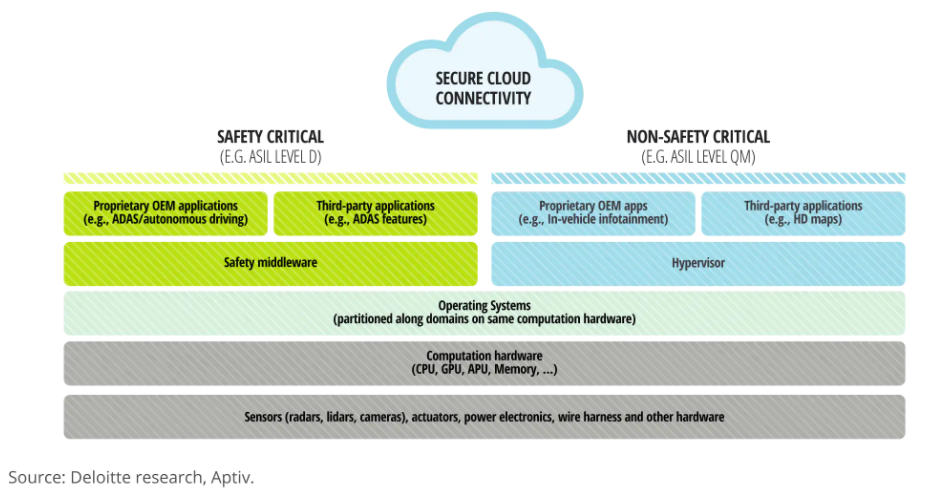
\includegraphics[width=\textwidth]{architecture}
    \caption{Architecture g\'en\'erique}
    \label{fig:archi}
\end{figure}
\url{https://www2.deloitte.com/us/en/insights/focus/future-of-mobility/pure-play-software-in-automotive-industry.html}
\FloatBarrier

Bla bla bla


\section {Le risque cybers\'ecurit\'e pour l'automobile}
 \medskip
 {\Huge L}'ajout de logiciels et de connectivit\'e....


3 niveaux d'attaques:
\begin{itemize}
\setlength\itemsep{1em}
\item \emph{Attaques physiques}. 
\begin{itemize}
\item Attaque via la prise diagnostique de la voiture. L'objectif est de pouvoir modifier les caract\'eristiques de la voiture et/ou de rajouter des options sur la voiture. Les logiciels d'une voiture sont hautement configurables. Un m\^eme logiciel est install\'e sur plusieurs gammes de v\'ehicules d'un constructeur. La diff\'erenciation entre les deux mod\`eles s'effectue par le param\'trage du logiciel. Si un attaquant \`a la possibilit\'e de modifier ces param\`etres, il peut activer des fonctions optionnelles de la voiture ou modifier les caract\'eristiques moteur pour booster le v\'ehicule.
\item Attaque via la prise USB de la voiture. L'objectif est de pouvoir cr\'eer un point d'entr\'ee pour une attaque courte ou longue port'ee sur le v\'ehicule. La prise USB peut \^etre connect\'ee sur un \'equipement radio qui permet d'\'etendre la port\'ee de l'attaque.
\end{itemize}

\item \emph{Attaque courte port\'ee} L'objectif est de pouvoir prendre le contr\^ole du v\'ehicule, d'envoyer de fausses informations ou de bloquer les communicatiosn aux v\'ehilcules aux alentours. De plus en plus de voitures ont un syst\`eme d'ouverture de portes et de d\'emarrage sans cl\'e.Par exemple, votre voiture est gar\'ee devant votre maison et les cl\'es sont sur le petit d'entr\'ee.  Un attaquqant peut ins\'erer un \'equipement radio entre la cl\'e et la voiture (attaque par relais). Un c\^ot\'e est proche de la voiture, lautre c\^ot\'e est connect\'e \`a une antenne scannant les fr\'equences radio de la cl\'e. Ceci permet d'ouvrir et/ou de d'emarrer la voiture m\^eme quand les cl\'es du v\'ehicule sont hors de port\'ee de la voiture. Une fois que l'antenne a accroch\'e la fr\'equence de la cl\'e, elle relaye son signal sur l'\'equipement proche du v\'ehicule. La voiture a ainsi l'impression que le propri\'etaire est proche et ouvre les portes et autorise la d\'emarrage. Le v\'ehicule peut \^etre vol\'e sans effraction (voir \url{https://www.youtube.com/watch?v=_cua7BFX-Qk} pour un video d'attaque relais). Un autre exemple, consiste \`a brouiller le signal pour la fermeture centralis\'ee d'un v\'ehicule. Le conducteur appuie sur le bouton de fermeture centralis\'ee de sa cl\'e, il a le sentiment que sa voiture est correctement ferm\'ee. Mais si le signal est brouill\'e, la voiture est ouverte et un attaquant peut facilement ouvrir un porte pour voler des affaires dans la voiture.
 
\item \emph{Attaque longue port\'ee}. L'objectif est de prendre le contr\^ole \`a distance d'un v\'ehicule. Un des fameux exemple de ce type d'attaque est la prise de contr\^ole d'une Jeep Cherokee par 2 attaquants; Andy Greenberg conduisait sa voiture sur l'autoroute vers Saint-Louis, roulant \` 70 mph. 2 hackers Charlie Miller et Chris Valasek sont install\'es dans leur canap\'e avec leur laptop ouvert. Dans un premier temps, la climatisation de la voiture s'est affol'ee, puis, une image des 2 hackers est apparue sur l'\'ecran de la voiture, la radio a chang\'e de station et le volume a fortement augment\'e, Mr Greenberg ne pouvait pas contr\^oler le volume de la radio ni la station. Ensuite la voiture s'est arr\^et\'ee toute seule. (voir \cite{Mil2015} pour le d\'etail de l'attaque)
\end{itemize}



\section {Car architecture over time }

\begin{figure}[h]
    \centering
	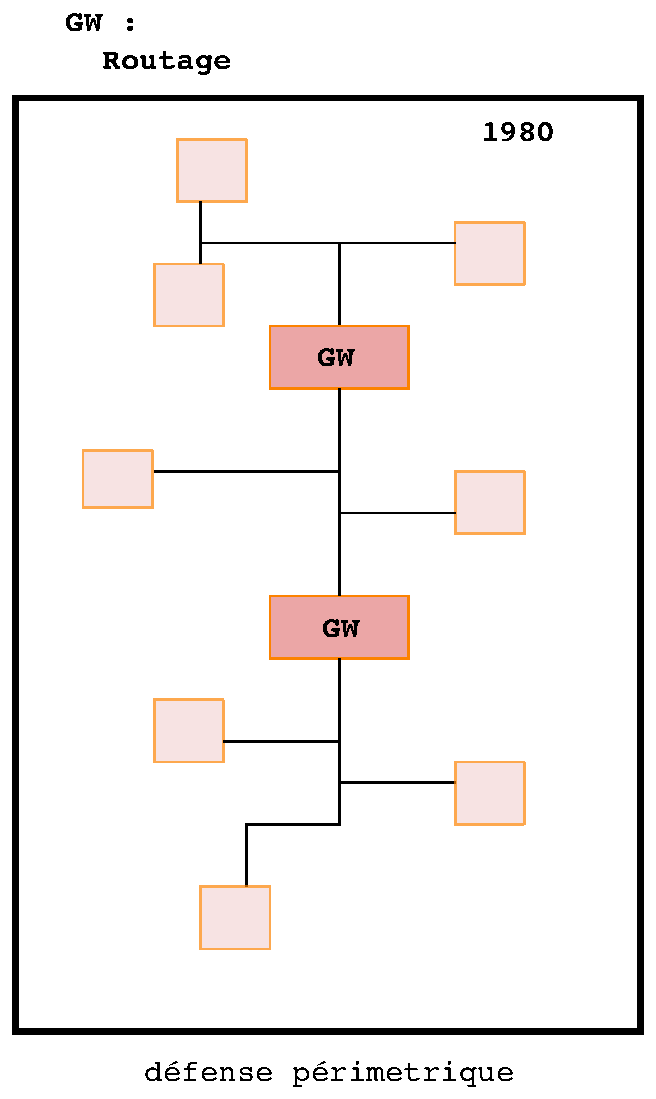
\includegraphics[width=0.45\textwidth]{schema/architecture/1980.pdf}
    \caption{Architecture 1980}
    \label{1980_archi}
\end{figure}

\begin{figure}[h]
    \centering
	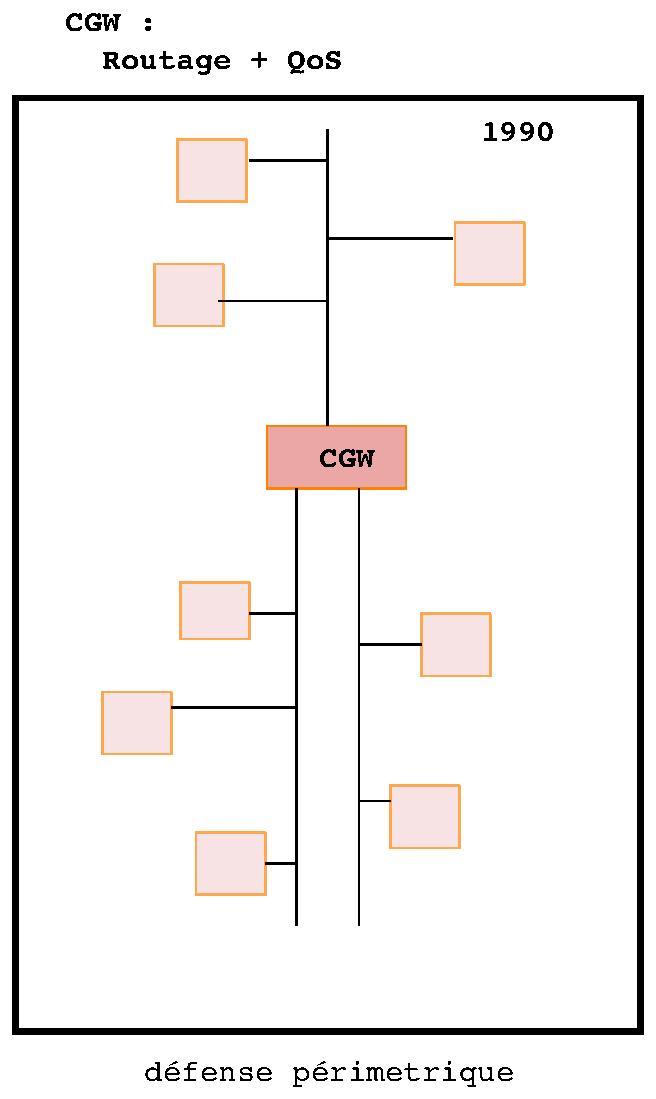
\includegraphics[width=0.45\textwidth]{schema/architecture/1990.pdf}
    \caption{Architecture 1990}
    \label{1990_archi}
\end{figure}

\begin{figure}[h]
    \centering
	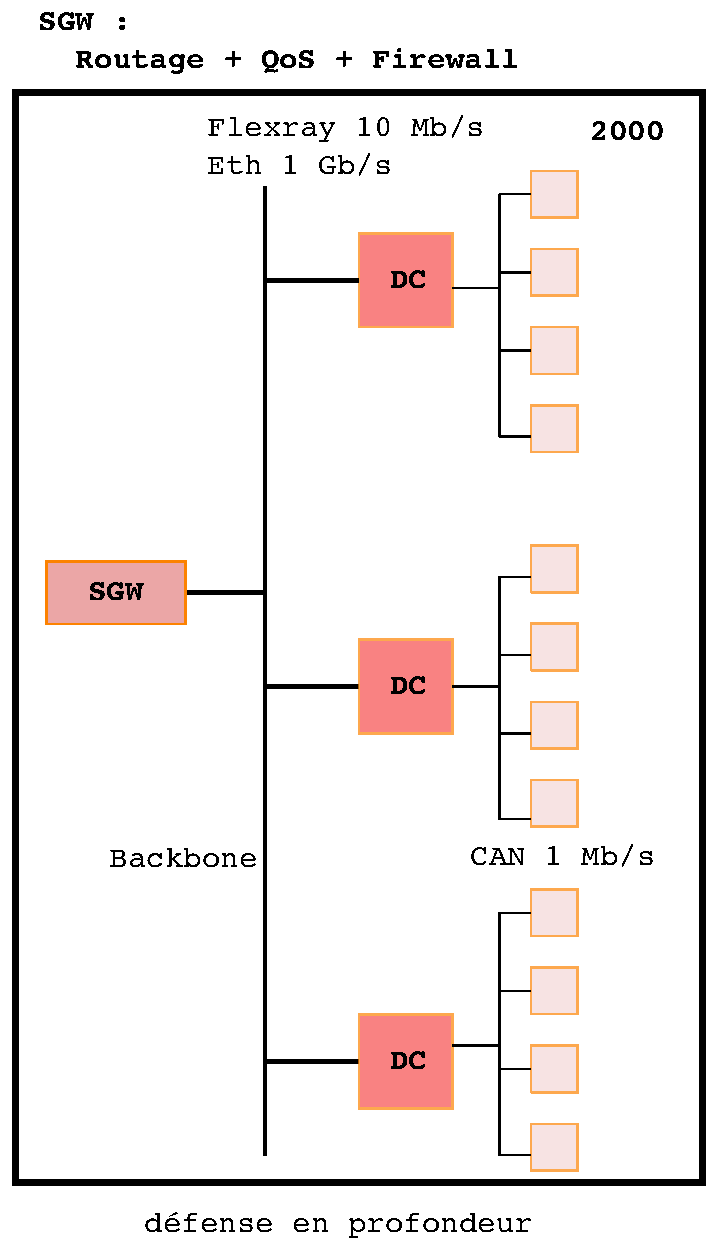
\includegraphics[width=0.45\textwidth]{schema/architecture/2000.pdf}
    \caption{Architecture 2000}
    \label{2000_archi}
\end{figure}

\begin{figure}[h]
    \centering
	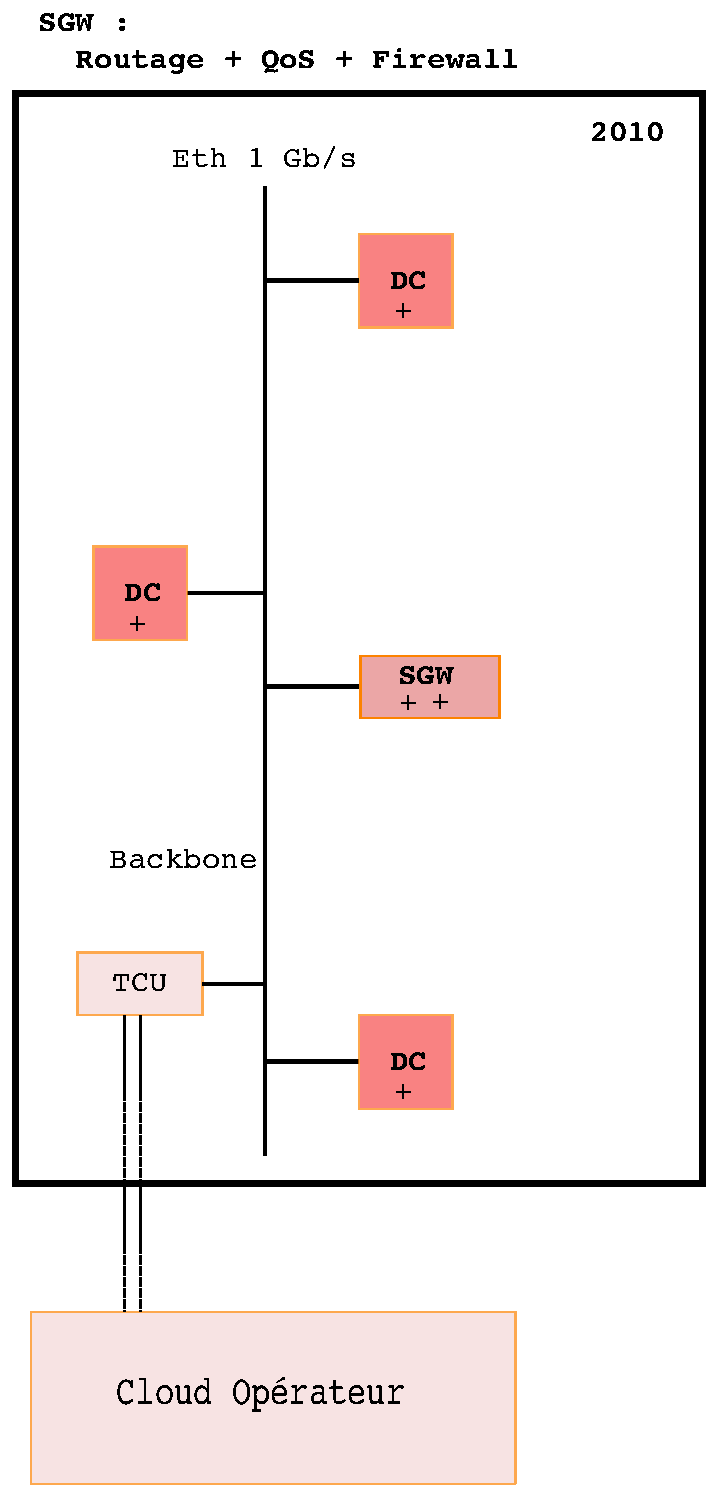
\includegraphics[width=0.45\textwidth]{schema/architecture/2010.pdf}
    \caption{Architecture 2010}
    \label{2010_archi}
\end{figure}

\begin{figure}[h]
    \centering
	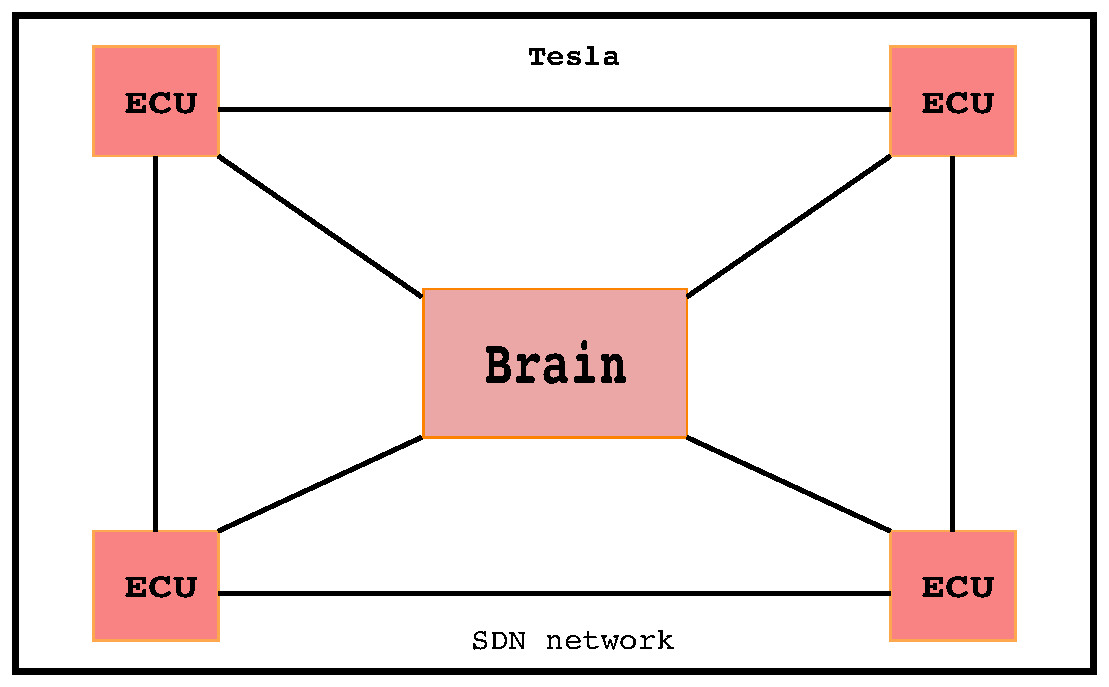
\includegraphics[width=0.6\textwidth]{schema/architecture/tesla.pdf}
    \caption{Architecture tesla}
    \label{tesla_archi}
\end{figure}



\section {Car Architecture we used}

\begin{sidewaysfigure}[h]
    \centering
	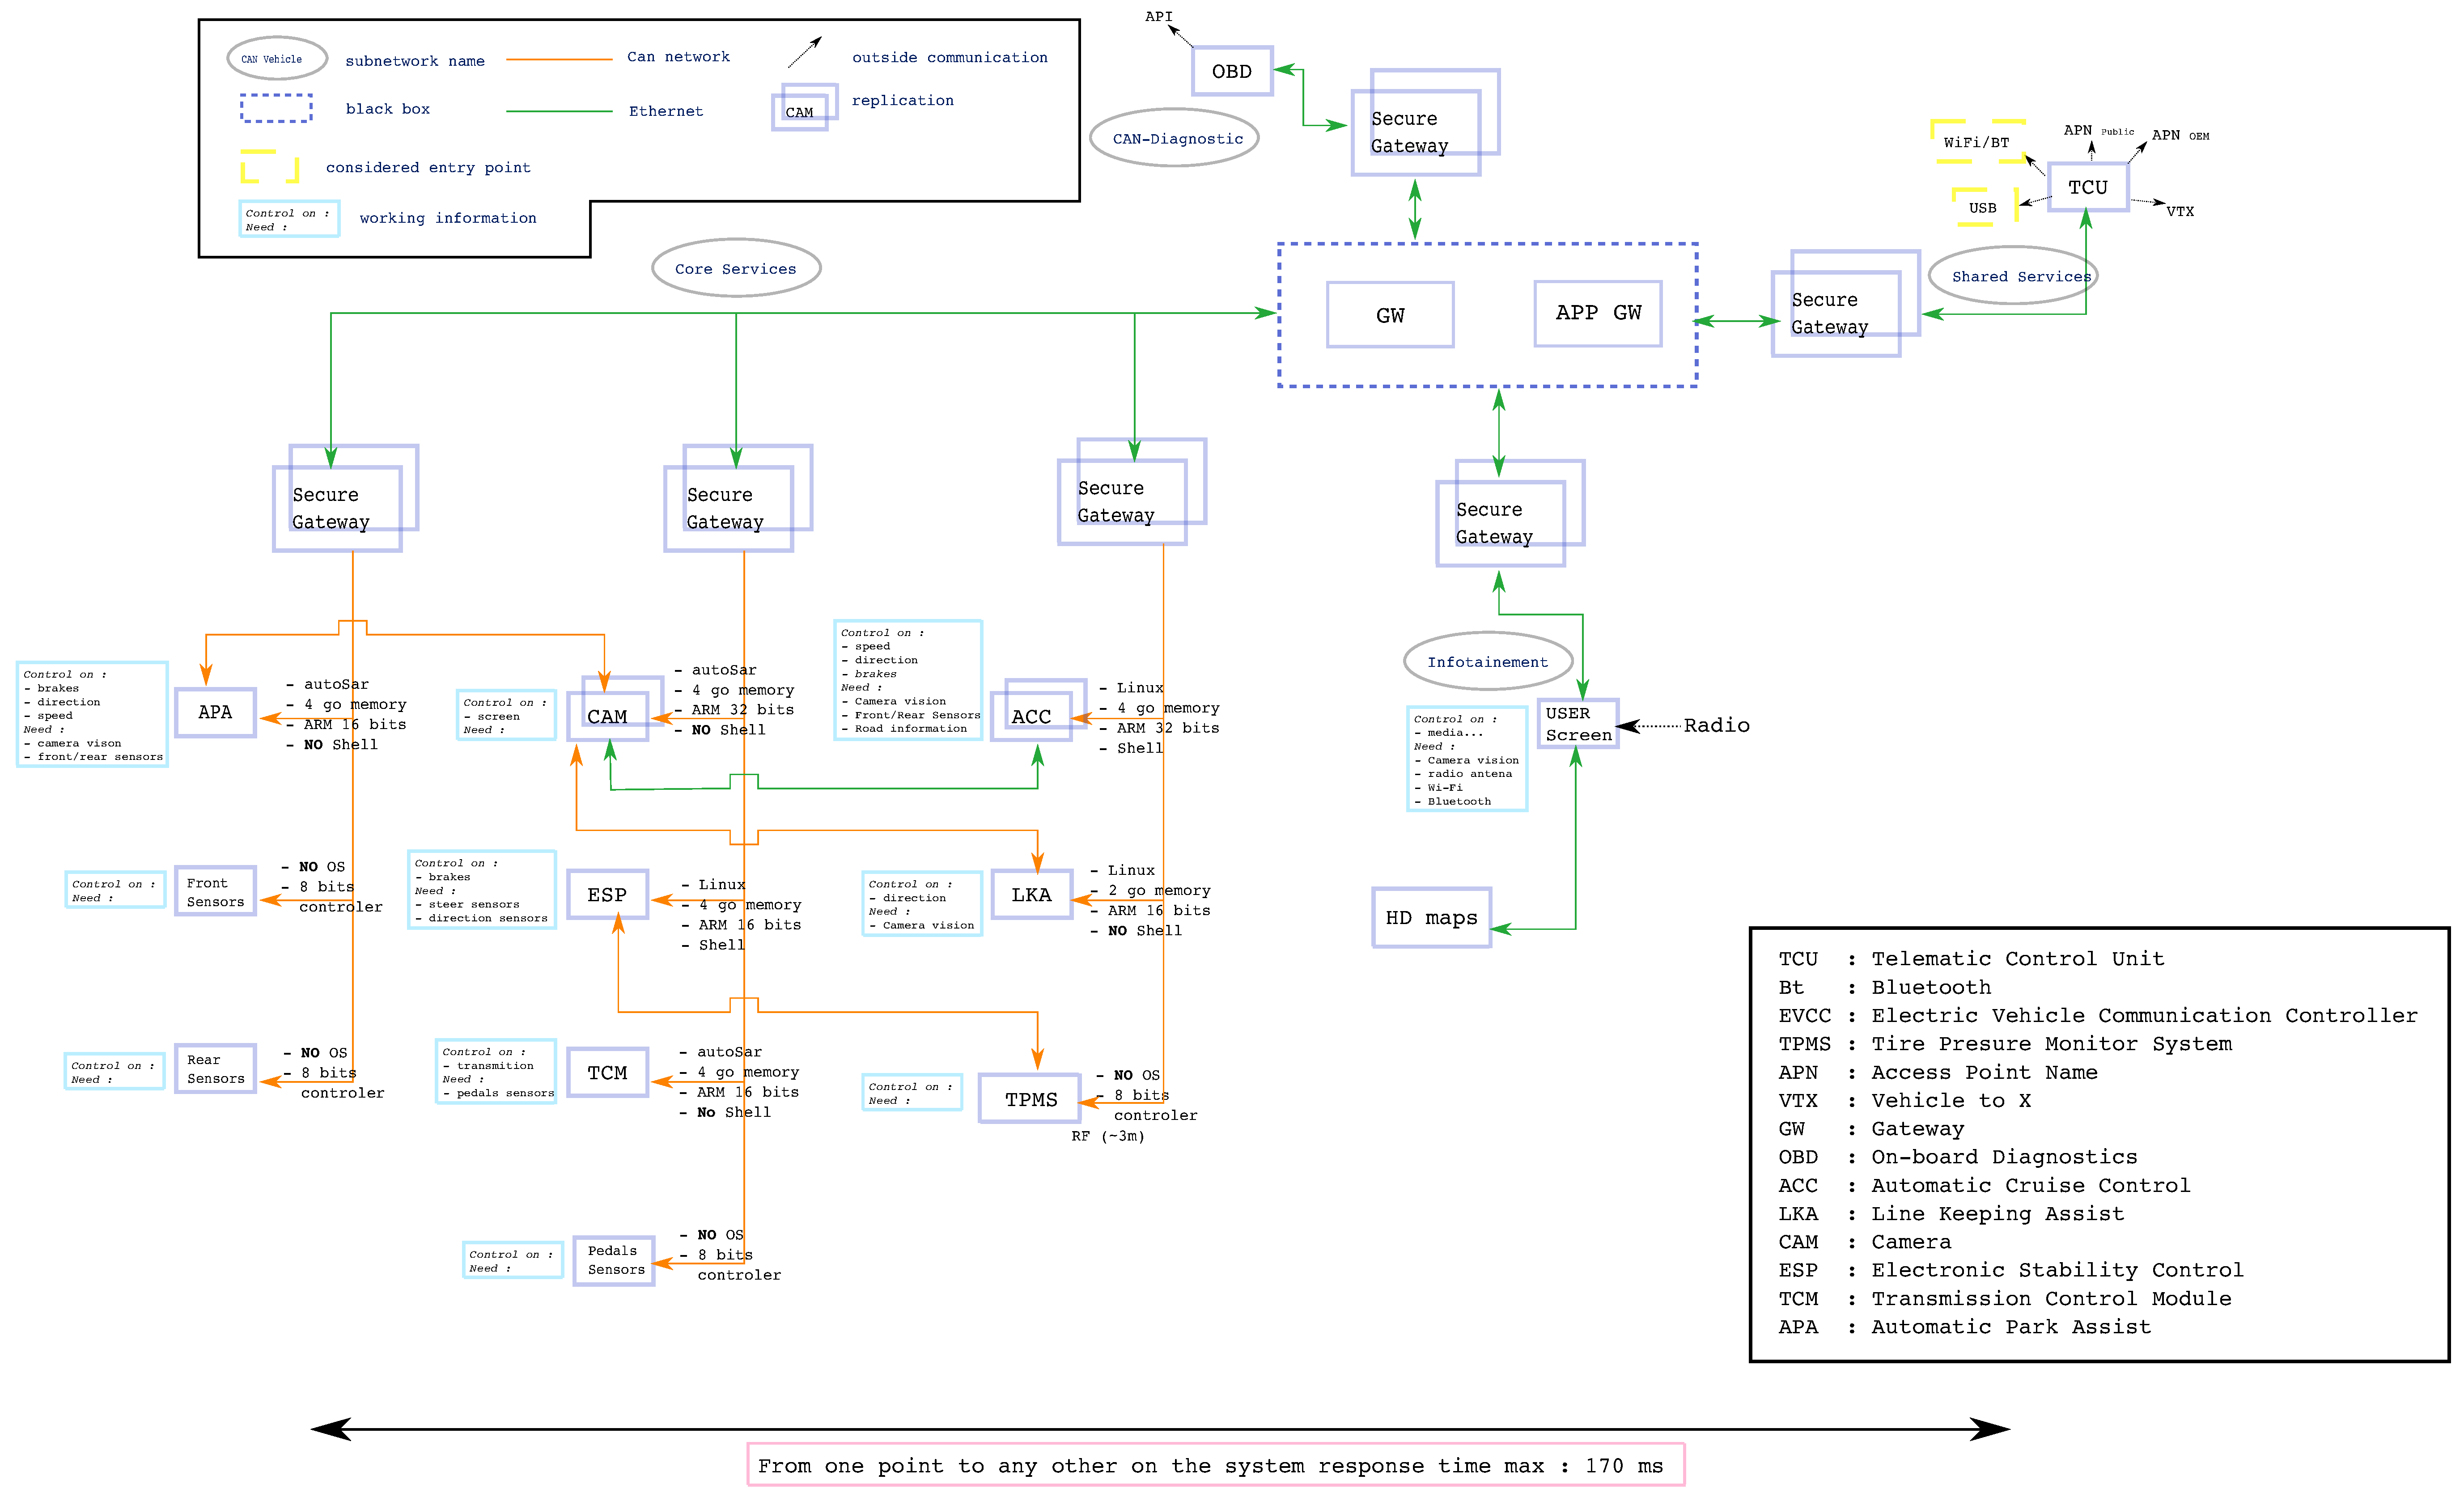
\includegraphics[width=1\textwidth]{schema/architecture/Car_complete_architecture.pdf}
    \caption{The architecture we used}
    \label{used_archi}
\end{sidewaysfigure}




\section {Existing Attacks}

\section {Existing Defense}



\chapter{Dynamic IPv6 addresses Switching} \label{MTDIP}
\smallskip
\hfill
\begin{minipage}[b]{8cm}
%{\it This work was presented in part at the conference of one-legged deaf-mutes in Quiberon in April 1994.}
\end{minipage}
%\begin{flushright} Remoi \end{flushright}
\vskip 2cm

\section{Problem Statement}
\label{sec:ps}


{\Huge I}n this article, we focus on techniques aiming at mitigating the risk
of attacks coming from an object's connectivity. In particular, we
concentrate on attack entrypoints induced by their Internet
connection. We consider two types of attackers: (i) attackers
connected to the Internet and seeking to infect a fleet of connected
objects via their own Internet connection; (ii) attackers connected to
the same subnetwork as the target objects.

On the one hand, attackers located outside the subnetwork of connected objects
are forced to scan the address range of this subnetwork in order to find the IP
address of some existing objects. On the other hand, attackers located inside
the subnetwork can \emph{see} the IP address of connected objects, since the
address is transmitted in plain text in the header of \emph{each} packet. The
latter is even more plausible for connected objects on sale for the general
public, \emph{e.g.} connected cars, which share a common network. Therefore, an
attacker located inside the respective subnetwork does not need to scan the
subnetwork and can launch his or her attack faster.

In this paper, we address the following problem: \emph{how to escape
from an attacker inside the subnetwork of an objects' manufacturer while
being hidden from attackers targetting these objects from outside
their subnetwork (i.e. from the Internet)}?

In this problem, \emph{escaping} refers to the capacity of an object to actively move
away from an attacker using MTD, while hiding refers to the passive capacity
of an object to be difficult to identify.

Of course, other objectives have to be considered when answering this
problem, *e.g.* limiting the impact of the defense mechanism on cost and
Quality of Service (QoS) of an object's Internet connection.

Compared to existing approaches pursuing the same objective
~\cite{antonatos_2007, jia_motag_2013, clark_2013, carroll_2014,fraunholz_catch_2018} the originality of our work
lies in the following characteristics: firstly, we not only consider
attackers proceeding from outside objects network, but also from
within this network. Secondly, we propose to limit the impact of
escaping techniques on the Internet connection QoS. Lastly, we
consider a more recent version of the Internet Protocol (IPv6). In the next
section, we present the technical foundations of the approach we
propose in this paper.


\section{Motivating Example}


\label{sec:motivating_ex}

{\Huge I}n order to illustrate the problem presented in section \ref{sec:ps}, we provide in
this section a motivating example: the network of connected cars. Actually,
connected cars are becoming a standard for car manufacturers as they aim at
selling more and more services such as navigation, entertainment, and driving
assistance applications directly integrated in the car.

Having access to the Internet, connected cars are thus visible from
any host connected to the internet, anywhere in the world. They are
thus exposed to threats considered as emergent in this market.

Connected cars are also a good example of connected objects where security
is a major issue: security patches are difficult to deploy, and
attacks may have catastrophic consequences for an entire fleet of
cars. As a consequence, in addition to applying security
countermeasures against known vulnerabilities, car manufacturers need to
consider the deployment of security counter measures that would
more generally repel potential attackers. We therefore investigate a
defense method based on MTDs to protect connected cars. Our objective is to reduce the risk of attacks
from the internet, considering attackers may be both inside or outside
the subnetwork that the cars are connected to: indeed, an attacker could buy a
car in order to connect it to the same network as the potential victims.

Beyond connected cars, other types of connected objects are also
critical and difficult to update, for instance in the context of
industrial automation, or in smart cities. The method we propose in this paper
is general enough to be adaptable to other types of critical
connected objects.




\section {Pool-based Ip address Switch}

{\Huge A}n attacker outside a
car manufacturer's subnetwork will have a great difficulty learning
the IP addresses of potential target vehicles. However, assuming that
an attacker owns a connected car, he or she can use it to connect to
the same subnetwork as all the other cars by the same manufacturer. It
is then possible for the attacker to use the car as a network terminal
and listen to messages circulating on the subnetwork. The IP addresses
of the sender and receiver of each message are visible in plain text
to every host connected to the subnetwork. Therefore, the attacker can
effectively bypass a network scan and directly harvest the IP
addresses of the cars communicating on this network. In this way,
attacks can be launched on a fleet of cars connected to this
network. In case of success, the attacker can potentially take control
of the entire fleet~\cite{valasek_adventures}.  In order to prevent this
scenario, our objective is to make it more difficult for an attacker
to attack a car via its network interfaces, from inside and outside of
the manufacturer's subnetwork.

\subsection{ Pool-based IP Address Switches}

\label{sec:pool_based_ip}

In this section, we describe an approach allowing a car on a
manufacturer's subnetwork to avoid attacks from within that
network. Following this approach, each car is assigned a pool of IP
addresses, allowing to switch among these addresses. We have designed
this approach in such a way not to lose the advantage of the large
IPv6 address range: cars remain hidden from attackers outside of the
manufacturer's subnetwork.

In order to find an optimal way to avoid attacks, several parameters
need to be considered. In the approach presented in more details
hereafter, a car is given a pool of $N$ IPv6 addresses. The greater
the number of addresses available to each car, the faster it can
switch addresses before returning to already used addresses and thus
hinder an attacker to understand and circumvent the defense.
Furthermore, if $N$ is too small, an attacker may easily launch a DoS
against most cars of the fleet.

Considering the time that each address is used (the IP address
switching period $P$), it must be sufficiently small to be effective,
such that an attacker will not have time to complete the attack before
the car switches to a new address accepting incoming messages. On the
other hand, the time $R$ before reusing an IP address from the pool
should be large, so that the attacker cannot easily predict the next
usable address too easily.

In order to optimize these two parameters, we need a large number of
IP addresses per vehicle ($N$) to allow more time to return to an
already used address and thus slow down potential denial of service
attacks. The number of network interfaces per car is limited by the
cost of a network interface. Also, if the number of interfaces and
thus of valid addresses is too large, a scan of the subnetwork from
outside this network will become easier (\emph{i.e.} reducing the benefits
of IPv6 addresses).


\subsection{Approach Principle}

The main principle of our approach is to equip each car with $N$
network interfaces, each of which is associated to an IPv6
address. Each address of each interface is an active address,
\emph{i.e.} it appears in the routing tables and can be accessed from
any other host connected to the Internet. However, the different
active addresses do not necessarily accept all incoming messages:
following the internal firewall rules of the car, some will be
accepted while others will be dropped. In our case, there is exactly
one network interface accepting incoming messages at any time.

As described in section \ref{sec:mptcp}, MPTCP allows a host to
declare several accessible paths. This makes it possible to optimize
travel times for packets if some transportation facilities are
saturated. In the context of this work, we are relying on MPTCP to
avoid loss of connectivity with services used by the car once its
address has changed. In order to do this, we declare all interfaces of
a vehicle, but only one possible path at any time, corresponding to
the accepting IP address.

The first time a car connects to the network, it broadcasts messages
over the entire subnetwork via its different network interfaces in
order to request IP addresses, which is the usual way to obtain a
valid address on a network ruled by a DHCP server. The DHCP server
responds to the car and assigns an IP address to each of its
interfaces. The car will then use MPTCP to declare the different IP
addresses belonging to it. In our approach, we propose to enrich the
connection protocol in the following way: The DHCP server sends to the
car an encrypted message containing the next IP address that will be
considered as the active address as well as the period of time during
which this address will remain active, call \emph{lease}. The car will then
edit the MPTCP rules to declare the new address received as the main
route to be used for all communications. The change will remain valid
until the end of the period received and the car will then again
change its current active address with the new address it will receive
from the DHCP server during this period.


The DHCP server manages the active addresses for each car. Every time
an active IP address reaches the end of its lease, the server picks a
new IP address from the car's address pool. Furthermore, it picks a
new duration for the new lease of this address. This duration
is drawn randomly from a predefined interval (noted \emph{[$a$,$b$]} and
centered around P). Randomization is necessary to prevent an attacker
who is listening on the network to anticipate and circumvent the
defense mechanism. The new active address and its lease
are sent to the car in an encrypted message, which can only be
decrypted by the destination car. All other network participants can
only see a message from the DHCP server to this particular car. After
receiving the encrypted message, the car updates its internal firewall
rules in order to accept messages on the new address, and changes the
MPTCP rules to declare the new external route corresponding to the new
address.

\begin{figure}[t]
    \centering
	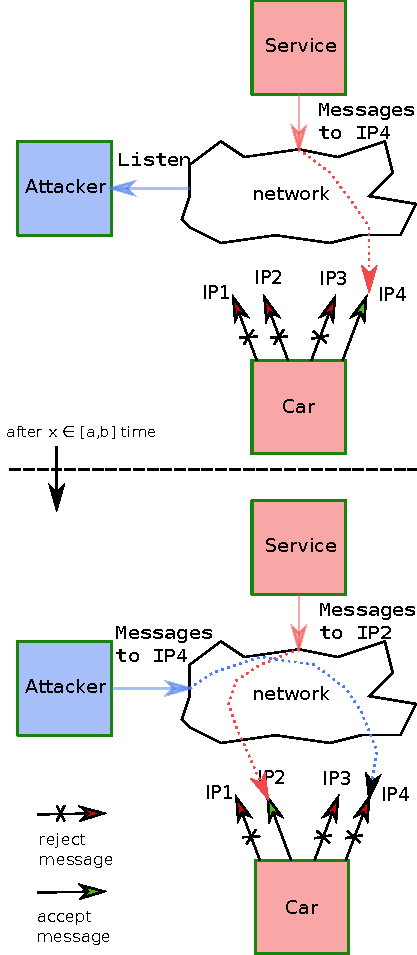
\includegraphics[width=0.3\textwidth]{schema/new2.pdf}
    \caption{Illustration of the proposed pool-based address switching scheme}
    \label{second}
\end{figure}

\subsection{ Example}

Figure \ref{second} illustrates a manufacturer's subnetwork, with a
connected car equipped with four network interfaces with each one an
IP address assigned, \emph{IP1}, \emph{IP2}, \emph{IP3}, and \emph{IP4}, as well as an
external service and an attacker connected to the subnetwork. In the
beginning, \emph{IP4} is the active IP address that accepts incoming
messages, while the other three reject all incoming messages. The car
communicates with the service, which responds by sending messages to
\emph{IP4}. Since the IP address of the car is visible in the header of any
circulating message in the network, the attacker can discover the IP
address of the car and may try to communicate with the car via
\emph{IP4}. Once the active time period of \emph{IP4} ends (after $x \in [a,b]$
time units), the DHCP server elects the new IP address accepting
messages, and sends -- in an encrypted message -- the new
configuration to the car. As shown in the lower part of the figure,
\emph{IP2} now becomes the active address, while \emph{IP4} will drop any
incoming messages.


\subsection{Protection}

If the attacker launches the attack before the currently receiving IP
address expires, he or she can start to communicate with the
discovered car. If the valid time period per IP address is short
enough, the address switch will take place before the attacker can
complete a successful attack. Assuming that an entire fleet of
vehicles is equipped with the proposed MTD mechanism, a massive
parallel attack against the whole fleet will be impractical: if the
attacker assembles a hit-list of collected IP addresses, these will
likely have changed at the time the attack starts. Since the
assignment of the receiving IP addresses and their active time window
is sent encrypted, the attacker will not be able to learn which
address the car has switched to once the currently active interface
stops responding.


As a conclusion, changing the IP address slows down an attacker coming
from inside of the subnetwork. This attacker will see the IP addresses
of the different cars communicating on the subnetwork. If he or she is
seeking to retrieve information about one discovered car before
launching his or her attack, he or she may even not be able to launch
his or her attack at all. By periodically changing the address, this
makes the time available for an attacker to perform his or her attack
shorter than without this mechanism.

\subsection{Cost} 

The presented defense mechanism can easily be implemented on top of an
existing network. It does not entail major infrastructure changes nor
heavy network trafic overhead. To apply this method in an existing
system, it will be necessary to setup *MPTCP* on the side of the
vehicles. Furthermore, it requires adding $N$ new physical network
interfaces on each car and adapting the car's firewall rules. On the
side of the network infrastructure, it will be necessary to slightly
modify the DHCP server for each subnetwork in order to implement the
assignment of an address pool to each newly connecting car and the
address renewal mechanism choosing a new address from the pool.

\subsection{ Discussion} 

It can be argued that the addition of several IP address would
facilitate the discovery of a fleet of vehicle from outside the
network, and this is actually the case.  The time to reach a 50\%
probability of finding one of the IP address is $3 \cdot 10^{12}$ s,
or 95 years instead of 951.  This remains a very acceptable
time. Especially since when an attacker succeeds in finding one of the
vehicles, there is only a $1/N$ chance that this IP address is the
active IP address that receives the messages.


This technique is able to repel attackers even from inside the network
if the period of IP address change is sufficiently small. However,
there remains a risk of \emph{Denial of Service} (DoS) attacks. This
vulnerability is due to the fact that each car is assigned a
\emph{static} address pool from the beginning to the end of its
connection on the network. This means that the addresses from this
pool will be used several times as the accepting address for incoming
messages.  This periodic re-use of the same addresses allows an
attacker to establish a list of known addresses and to flood them with
messages continuously, resulting in a denial of service. Therefore, an
alternative approach -- which will be presented in the following --
limits address reuse.

\section{Randomized Pool-based IP Address Switches}

\label{sec:second}

{\Huge I}n this section, we describe an alternative MTD approach that
additionally aims to protect the connected vehicles against DoS
attacks, while trying to limit the impact on the network
infrastructure. We keep the same assumptions about the system: all
cars of the same manufacturer are connected to the same IPv6
subnetwork controlled by the manufacturer; each car has $N$ network
interfaces providing it with $N$ IP addresses on this
network. Likewise, we are still using MPTCP to maintain several open
connection paths as well as the periodic change of the IP address
accepting messages. However, we make the address pool associated with
each car dynamic, i.e. addresses will change over time, such that no
address will be used twice by the same car, in order to avoid DoS.


\subsection{Approach principle}


As before, at the first connection of a car on a network, the DHCP
server assigns an IP address to each of its interfaces and indicates
the interface that will accept incoming messages.

However, in addition to regularly switching the active interface of
each car, the DHCP server will send an encrypted message, ordering the
receiving car to replace the IP address of one of the \emph{inactive}
interfaces with a fresh one. The car needs to do the necessary changes
in its configuration, and update the corresponding interface to use
the new address once it will become the active interface. This implies
also adding the new address to the MPTCP rules as a new route to the
car. In order to avoid packet loss, and give the car sufficient time
for reconfiguration, the address change occurs \emph{in the
background}, \emph{i.e.} it never affects the currently active interface and
does not interfere with the car's communication.

The period by which new addresses will be assigned can be chosen freely, leading
to different trade-offs of costs and security. If it is longer than the validity
period, this will lead to address reuse. By always renewing the address of the
least recently deactivated interface, the address pool of size N is completely
renewed every N address changes. As a consequence, no address will ever be
active twice\footnote{unless the same address is randomly chosen twice by the
DHCP server, which has a sufficiently low probability.}, as illustrated by the
following example.

\begin{figure}[h]
    \centering
	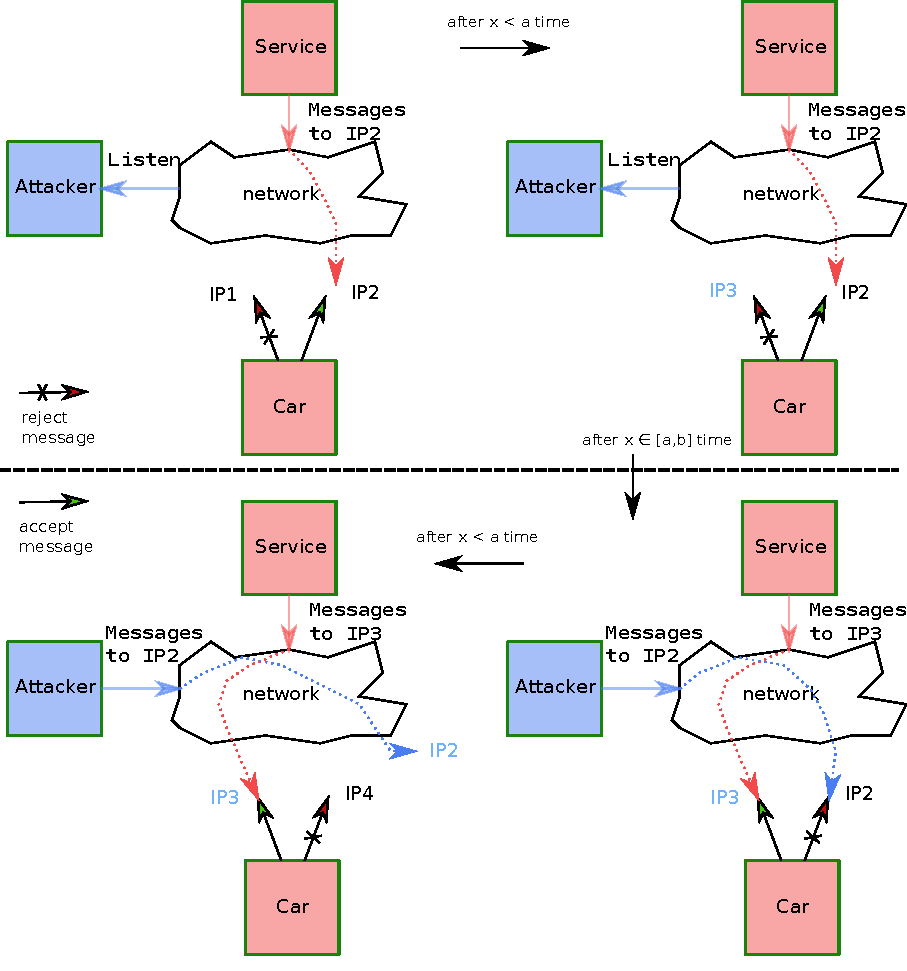
\includegraphics[width=0.6\textwidth]{schema/new4.pdf}
    \caption{Illustration of the randomized pool-based address switching with 2 network interfaces per vehicle}
    \label{third}
\end{figure}

\subsection{ Example}

Figure \ref{third} shows the randomized address switching for the case
$N=2$, i.e. each car has two network interfaces. The car *Car* is
connected to the manufacturer's subnetwork and has currently addresses
IP1 and IP2 assigned to its interfaces, where IP2 is the address
accepting incoming messages. the \emph{Car} communicates with a service on
the network, while an attacker listens to the network
traffic. Meanwhile the *Car* receives instructions from the server to
replace the address IP1 with the fresh address IP3, so it updates its
interfaces, MPTCP rules and firewall rules. Once the valid time period
of IP2 expires, IP3 becomes the active address accepting incoming
messages, while the attacker still tries to communicate via IP2. The
*Car* continues its communication with the service while the
attacker's messages are rejected on IP2. Meanwhile, the car then
receives instructions to change IP2 to IP4, so the attacker now talks
to an unknown address. By changing addresses at each time period, the
attacker only has this period to launch his or her attack and can no
longer anticipate changes in the \emph{Car's} addresses.

\subsection{Costs}

If the address renewal period is equal to the validity period -- as in
the above example -- each address is only used once. Thus, there is no
need to choose $N$ greater than two, as this does not increase the
entropy. Therefore, the constant costs related to the number of
network interfaces are lower than in the static pool-based approach
with $N > 2$. However, there is an additional overhead for the network
infrastructure: firstly, there are additional address renewal messages
sent out by the DHCP server. Secondly, the DHCP server itself has
additional work to do choosing new addresses and changing its internal
routing tables.

\subsection{Randomization on Demand}

An alternative application of the randomized address-renewal would be
to use it in addition to the first method. In other words, equipping
the cars with $N$ network interfaces with addresses assigned per
interface that do not automatically change over time. But when a
persistent attack on the network is discovered, an address renewal is
triggered: for the list of vehicles under attack, the pool of
available addresses is updated, thus preventing denial of service.


\begin{figure}[h]
    \centering
	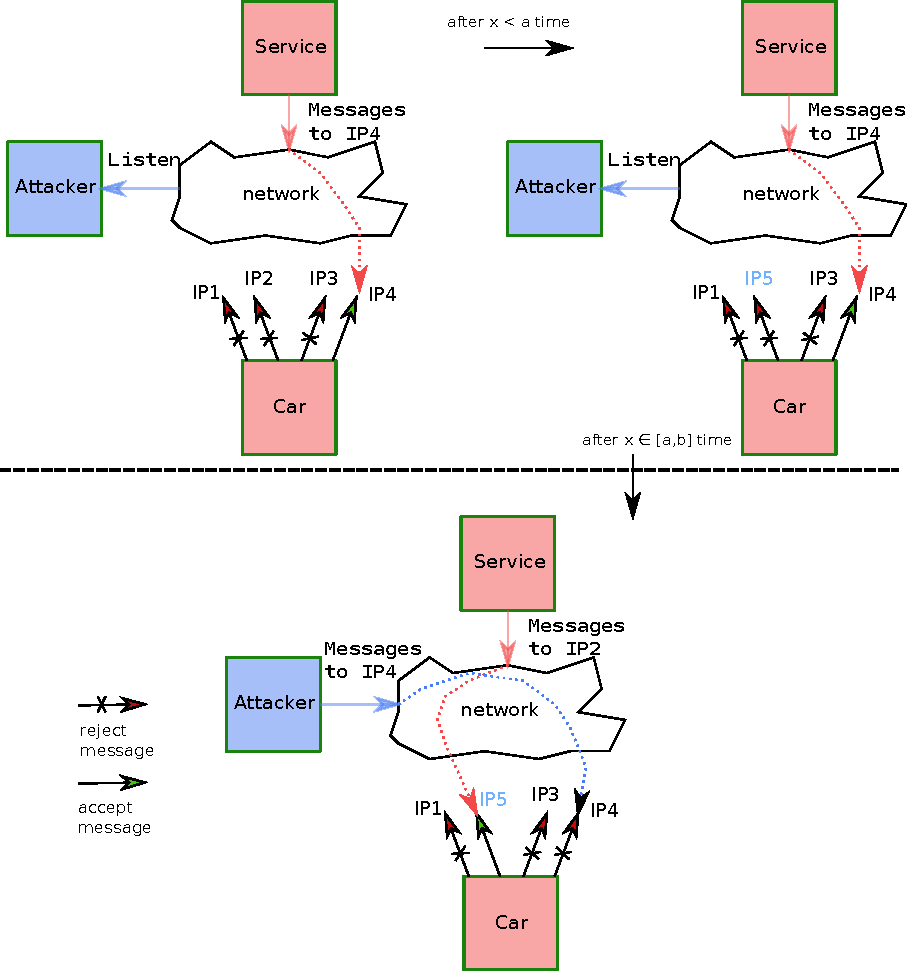
\includegraphics[width=0.65\textwidth]{schema/new3.pdf}
    \caption{illustration of the method with N network interfaces per vehicle}
    \label{Random1}
\end{figure}

Figure \ref{Random1} illustrates this
combined approach. There is a car connected to the subnetwork with 4
network interfaces, corresponding to the IP addresses IP1, IP2, IP3,
and IP4. In the beginning, IP4 is the only address accepting incoming
messages. As before, an attacker is listening to messages circulating
on the network. Upon detection of the intruder, the car receives
instructions from the DHCP server to change IP2 address to IP5, and it
updates the MPTCP and firewall rules. At the end of the validity
period IP5 becomes the new accepting address.  The attacker will try
to attack IP4 which no longer accepts incoming messages.  In contrast,
in the absence of a detectable threat, the address pool will remain
stable, avoiding additional network traffic and server load.

\subsection{Discussion} 

By adding randomized renewal, DoS attacks can be thwarted, with higher
costs incurred by network traffic overhead and increased DHCP server
load. Between the two extremes -- no address renewal at all or after
each interface swap -- the renewal period can be chosen in order to
adapt the overhead and the security level to the use case and
available infrastructure. As an alternative, addresses can be renewed
on demand only, in combination with an appropriate attack detection
mechanism.



\section{Conclusion}

\label{sec:con}

{\Huge I}n this paper, we investigate a moving target defense in the context of
connected objects on an IPv6 network. In particular, we consider connected cars
sharing a common manufacturer's subnetwork, which makes them particularly
vulnerable to attacks from within the same network. 

As a remedy, we propose a dynamic address switching scheme relying on the
network's DHCP server. In our approach, each connected car disposes of several
redundant network interfaces, each with a separate IP address. This allows for
dynamic address switching without connection losses. The basic protection
mechanism is that each car only accepts incoming messages on one interface at
any time, leaving attackers talking to inactive addresses after a switch. While
the basic approach uses fixed address pools, an additional address renewal by
the DHCP server can help to thwart denial of service attacks, since it allows to
avoid address reuse. Adjusting both the periods for address switching and
address renewal leads to a flexible MTD approach that can be adapted to the
security requirements and network infrastructure at hand. To the best of our
knowledge, this is the first network MTD approach presented in the context of an
IPv6 subnetwork which considers attacks from within the same network.




\chapter{Game Theory usage} \label{GAMETHEORY}
\smallskip
\hfill
\begin{minipage}[b]{8cm}
%{\it This work was presented in part at the conference of one-legged deaf-mutes in Quiberon in April 1994.}
\end{minipage}
%\begin{flushright} Remoi \end{flushright}
\vskip 2cm

{\huge I}n the automotive domain, there is a clear trend towards increased connectivity: Many new services are available today which demand a reliable communication between the car and its owner (e.g.~via smartphone applications), the manufacturer, or even the infrastructure. Many cars offer a local WiFi network and Bluetooth. Furthermore, semi-autonomous driving -- such as parking and lane keeping assistants or automatic emergency braking -- is now standard in middle to higher class models. These functionalities require a large number of sensors such as cameras, radars or other distance sensors. While these services are supposed to increase the safety of the passengers (and of pedestrians), they entail new security risks. Indeed, many attacks have been demonstrated in the recent years, some of them putting the life of the car's passengers at risk \cite{smith_car_2016}. 

The security of connected cars is taken very seriously by the manufacturers and it has become a major design goal. For instance, in a typical system architecture of a connected car, the subsystems are divided into different domains, and any message crossing a domain-border passes through a secure gateway. This allows to filter unauthorized messages and prevent an attacker who has compromised one subsystem from spreading to other -- more critical -- subsystems. However, such protections are of a \emph{static} nature. The defenses are programmed and configured once before the car leaves the factory. Because of strict certification requirements, software updates are very costly and usually must be performed by licensed workshops. This makes the relation between potential attackers and the system under attack an \emph{asymmetric} one: The attacker can analyze the car's system in order to find vulnerabilities and prepare an exploit that can then be applied -- potentially to a whole fleet of cars in parallel.   

In order to minimize the risk of such large scale attacks, it is paramount to also consider \emph{dynamic} defenses. Moving Target Defense (MTD) is a family of defense technique that proactively changes the configuration of a system in order to deceive an attacker who relies on previously gained knowledge to find and exploit vulnerabilities. MTD mechanisms may reconfigure the network, runtime environment, data, or software of the target system. Combining such mechanisms, a defense strategy based on MTD should define \emph{where}, \emph{how}, and \emph{when} to reconfigure. Critical Real-Time Embedded Systems \emph{(CRES)} -- such as connected cars or other transportation domains -- are a particularly interesting application domain for MTD: Such systems are usually used for a very long time (10+ years), and are thus exposed to the discovery of new vulnerabilities and \emph{zero-day} attacks. In addition, as CRES have limited resources (computation, communication, storage), and because their failures may have catastrophic consequences, these systems are difficult to defend using traditional methods. MTD can delay the implementation of attacks when new vulnerabilities are discovered, and limit their scope. This can be seen as a way to increase the \emph{resilience} of the attacked systems. We define resilience of a system as the capability to deliver its services in a safe way, even when faced with unknown attacks. This may be achieved by degrading certain services or by bringing the system to a safe state before critical damage has been done.   

So far, most works on MTD have focused on the question \emph{where} and \emph{how}, thus providing and evaluating new MTD mechanisms~\cite{xu_2014, taylor_automated_2016}.
Some studies have also been conducted in order to assess the efficiency of MTD in the context of risk analysis methods~\cite{hong_assessing_2016}. More recently, a few methods have been focused on the question of \emph{when} to reconfigure~\cite{lei_optimal_2017,sengupta_game_2017, feng_stackelberg_2017, li_optimal_2019, Zhang_Strat_2019}, but these contributions focus on the domain of web applications, therefore their requirements, MTD mechanisms, and models are not suitable for the design of CRES. 

Nevertheless, there exist several MTD mechanisms applicable to CRES, and for which the question \emph{how} is already answered. Instead, we focus on the questions of \emph{when} and \emph{where} to reconfigure parts of a system. 
Obviously, the question \emph{when} is actually: \emph{how often}? A question to which one may simply answer \emph{as often as possible}; but implementing an MTD mechanism has a cost, and its execution inevitably impacts the availability of the components that must be re-configured. For instance, switching IP addresses will induce communication overheads and temporary connection or packets losses. Therefore, MTD comes with an implementation cost and a quality of service (QoS) degradation.

In this paper, we aim at answering the following question: How to model MTD benefits and cost in order to find optimal MTD strategies (i.e.~\emph{where} and \emph{when} to move) in the context of CRES? We propose a combination of risk analysis techniques, MTD mechanisms, and a game-theoretic approach in order to define the best defense strategy to adopt in terms of frequency of each available MTD mechanism. 
The contributions of this paper are: 
\begin{enumerate}
    \item A game theoretic model for the defense of CRES
    \item A resolution method based on the transformation to an MILP problem
    \item A complete methodology to define the input parameters of the presented model
    \item An experimental case study for a typical connected car architecture
\end{enumerate}


\section {Motivating Example }

{\huge C}onnected cars are essentially critical and connected real-time embedded systems, that operate for an average of 15 years. 
These vehicles can be purchased by virtually anyone with a sufficient budget, including someone looking for a way to attack them. As a consequence, an attacker has time to study a specific vehicle and its defenses in order to discover vulnerabilities and ways to exploit them. 
An attacker who owns a vehicle can also use this vehicle to gain access to the manufacturer's network in order to mount remote attacks on vehicles on the same network. This could eventually allow to infect an entire fleet.

Regarding the security of connected cars, software updates are difficult to perform on these widely distributed systems with limited computation and communication capacities.
This means that car manufacturers must mainly rely on defenses deployed when the vehicle is sold or updated. 
The asymmetry between attackers and defenders is therefore very significant in the context of connected cars. 

\begin{figure}[h]
    \centering
    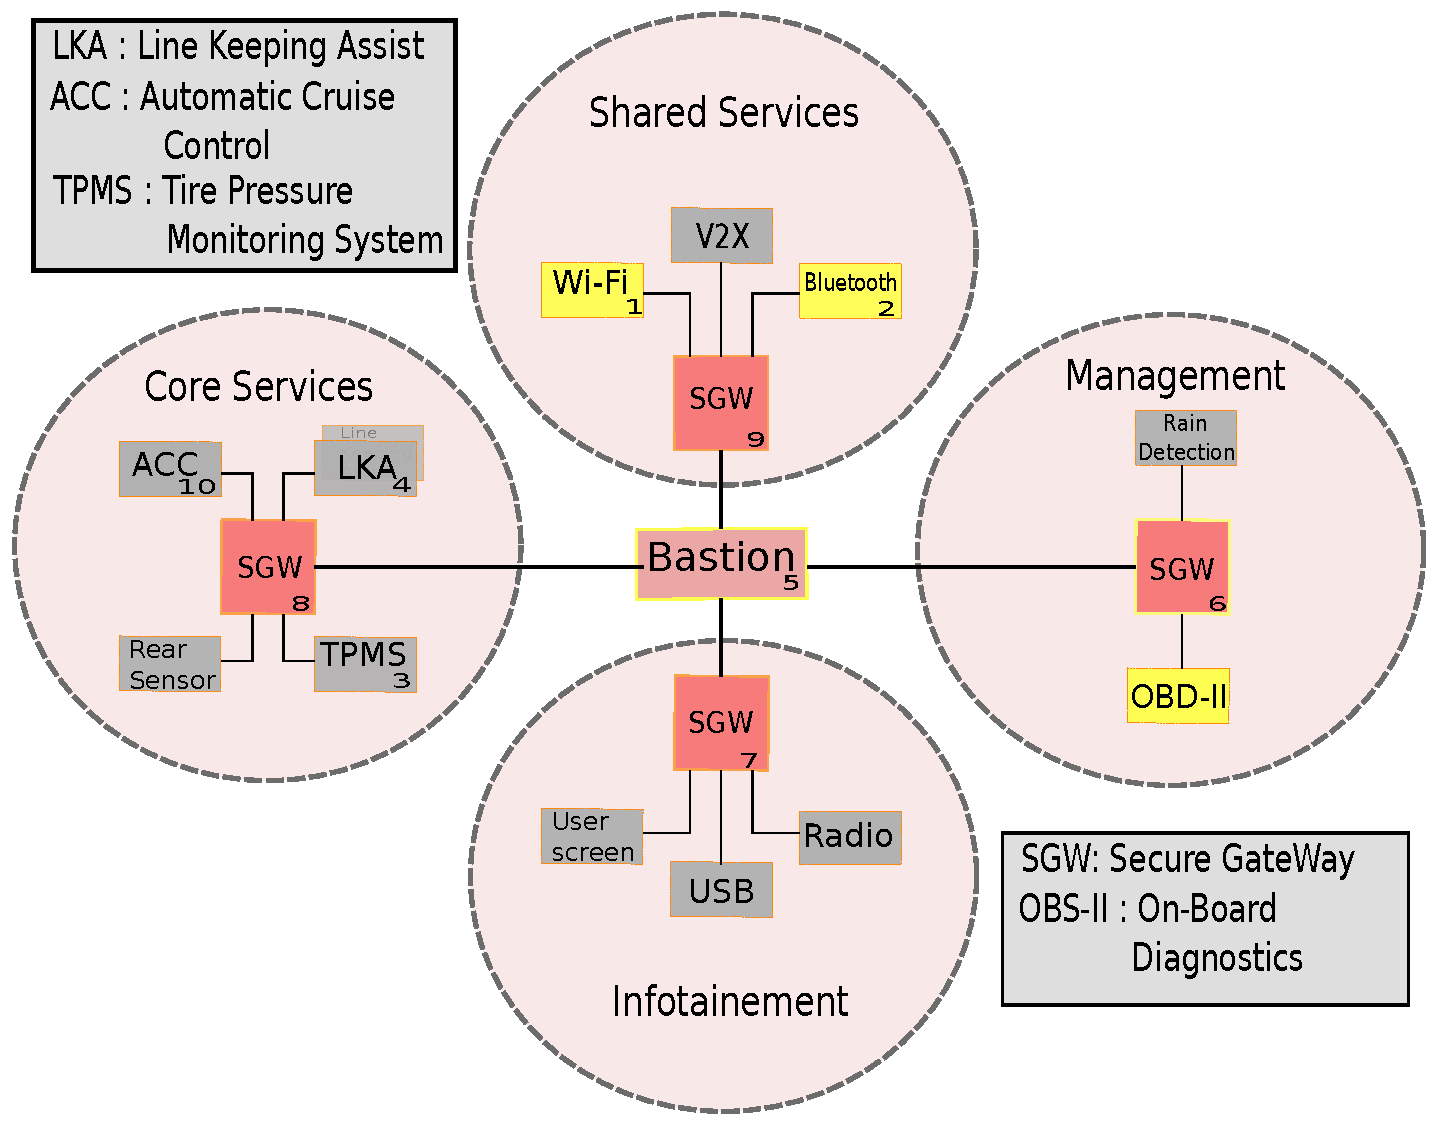
\includegraphics[width=0.7\textwidth]{schema/car_architeccture_compact.pdf}
    \caption{Vehicle Architecture scheme}
    \label{fig:game_archi}
\end{figure}

An example of the internal architecture of a connected car is presented in Figure~\ref{fig:game_archi}. This type of architecture is called \textit{architecture by domain} because the different services of the vehicle are separated into four domains according to their role:

\begin{enumerate}
    \item \textbf{Infotainment}: services related to the user experience such as the radio, the on-board screen, and various applications accessible to the user. 
    \item \textbf{Core Services}: critical services for the operation of the vehicle such as cruise control, brake controls, or lane keeping assistant.
    \item \textbf{Management}: services dedicated to diagnostics and updates of the vehicle, such as the OBD-II \textit{(On-Board Diagnostic)} plug. 
    \item \textbf{Shared Services}: regroups services allowing to communicate with the outside world (V2X) as well as some services shared among several domains.
\end{enumerate}

Within each of these domains, the communication is managed by a Secure Gateway serving as router and firewall. For example, in the Infotainment domain, if the USB module wants to send a message to the user screen module, those messages must go through the domain's Secure Gateway.

All the communication between two separate domains must pass through an entity called the \textit{Bastion}, operating as a \textit{"super" Secure Gateway}. If the Bluetooth module located on the Shared services domain wants to communicate with the user screen module located on the Infotainment domain, all the messages will be examined and filtered by the Bastion.
The \textit{Bastion} is basically a router and a firewall for the communication between the domains. Typically, it also embeds an IDS \textit{(Intrusion Detection System)} in order to detect any attempt of intrusion into the vehicle's system.

This architecture has been designed with safety and security in mind, and the vehicle already possesses some defenses located on the secure gateways. But these defenses are static, i.e.~they have a configuration that will remain the same throughout the entire life cycle of the vehicle. If an attacker finds a vulnerability and a way to bypass an existing defense, the attack has a high chance of being reproducible and may be applied to any number of vehicles of the same type. 

Consider as an example the access code to the vehicle's Bluetooth module -- providing an entry point for attackers that target the vehicles integrity -- and the Bluetooth MAC address, which is of interest for attackers that aim to compromise the driver's privacy (e.g.~by tracking the vehicle).
The Bluetooth access key is generated only once, allowing a trusted device to access the Bluetooth module. 
It is relatively easy for an attacker to retrieve the access key of this module. The attacker will then be able to use the recovered key to connect to the Bluetooth module and gain access to the CAN bus of the vehicle in order to send forged messages, potentially compromising the integrity of the vehicle.
The MAC address of the Bluetooth module is visible in clear to all nearby peripherals. Once the correspondence is made between the MAC address and the associated vehicle, it is possible to follow the comings and goings of this vehicle in the areas monitored by an attacker. 
 
The introduction of MTD on the Bluetooth module can help to limit such attacks, and thus to slow down the progression of an attacker.
For example, we can periodically change the access code to the Bluetooth module. By using a period smaller than the time necessary for an attacker to discover the access code, it becomes harder for an attacker to succeed in connecting to the vehicle's Bluetooth module.
Similarly, by periodically changing the MAC address of the vehicle's Bluetooth module, it becomes more onerous for an attacker to maintain a correspondence between a MAC address and a vehicle, making it more difficult to track. 

However, there is a drawback of using MTD in a connected vehicle. Indeed, connected vehicles are critical embedded systems with limited computing power and strong time and QoS constraints.
The use of MTD on a vehicle will have an impact on these three elements. It is therefore necessary to find a good balance between the protection of the vehicle and the operating constraints related to this type of system.
Therefore, we are interested in finding the best strategy for using the different MTD in the vehicle and thus be able to determine the frequency of use of each MTD on each asset, allowing the vehicle to be as well protected as possible against all types of existing and future attacks. 
As a solution to this problem, we propose a model representing the interactions between a set of attackers and a connected vehicle, as well as all the constraints that the system must respect.


\section {Model presentation}

{\huge I}n this section, we present our model, starting with the basic structure, and discussing the different input parameters in the following.

\subsection{Model Structure}

\label{game_struct}

The game we use will be represented by the tuple $<N, (M_i)_{i \in N}, P, R_{nmpn'm'}, \widehat{R}_{nmpn'm'}>$ in which: 

\begin{itemize}
	\item $N = \{0, 1,...,n\}$ : the set of nodes of the system under attack. 
	\item $M_i = \{0,1,..,m_i\}$ : the set of MTD defenses present on node $i$. 
	\item $P = \{0, 1,...,p\}$ : the set of attacker profiles.
	\item $R_{nmpn'm'}$ : reward obtained by the defender when he chooses to use the MTD $m$ on node $n$ while the attacker $p$ targets the MTD $m'$ on node $n'$.
	\item $\widehat{R}_{nmpn'm'}$ : reward obtained by the attacker $p$ when she chooses to use to target the MTD $m'$ on the node $n'$ while the defender will defend the node $n$ with the MTD $m$. \\
\end{itemize}


The game is composed of a set of nodes $N$ corresponding to the elements present in each domain, such as the SGW, the Bluetooth, or the ACC.
On each of these nodes, a set of assets is present, corresponding to  valuable information or subsystems. 
Each of these assets is protected by one or several MTDs of the set $M_i$.
The different attackers are represented by the set of attacker profiles $P$, each of which has the objective to target some assets present on the different nodes, depending on the profile type.

Resolving the game consists in finding the best defense strategy for the defender against the set of attacker profiles taken into account.
The decision variables of the problem corresponding to the strategies chosen by the two players and are represented as follows:

\begin{itemize}
	\item $\delta_{nm}$: The strategy of the defender on the node $n$ and its MTD $m$.
	\item $\alpha_{pn'm'}$: The strategy of the attacker of profile $p$ on the MTD $m'$ of node $n'$.
\end{itemize}

%On each node of the studied system there is potentially one or more assets that we want to hide from an attacker.
%In our game, we represent each node having at least one information to hide by a node. Knowing that each information can be protected by one or more MTD.

On each node, the defender has a budget of $1$ to spend. The distribution of this budget corresponds to the frequency of use of each MTD over a period of time and will be represented the decision variable $\delta_{nm}$.

Each attacker has a global budget of $1$ to spend on the whole game, and will choose only one node to target. As we will consider several types of attackers, each with different objectives to achieve, they will not necessarily all be interested in all the assets present on a node. 

\begin{figure}[h]
    \centering
    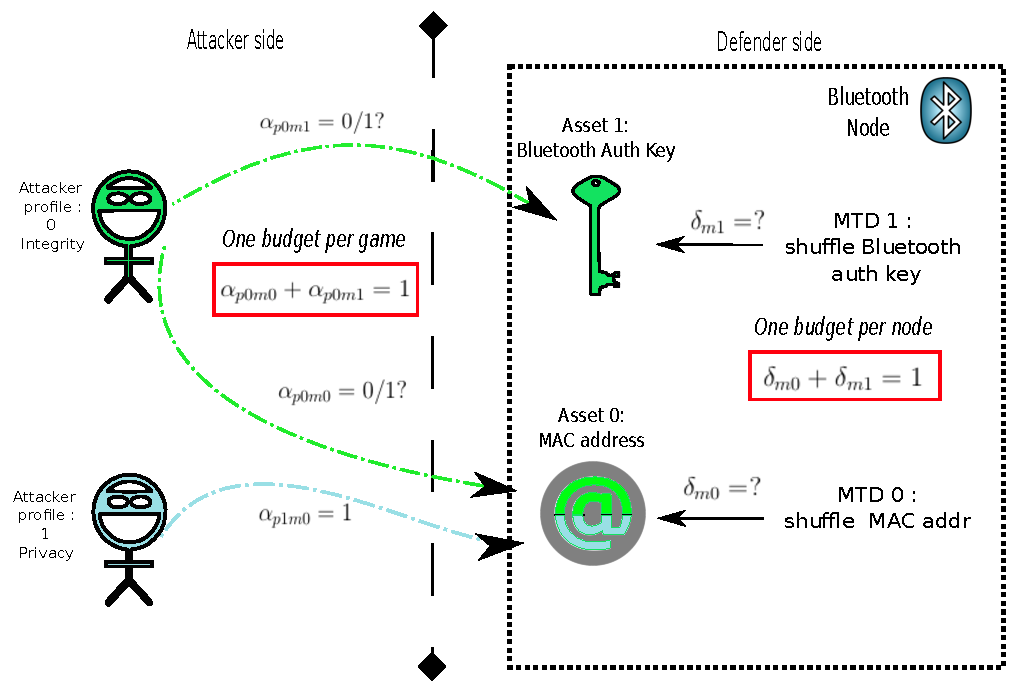
\includegraphics[width=0.95\textwidth]{schema/node_archi_3.pdf}
    \caption{Model Representation for one node and 2 attacker profiles}
    \label{fig:node_pres}
\end{figure}

To illustrate our model, Figure~\ref{fig:node_pres} shows a game composed of one node with two assets to protect and two MTD, as well as two attackers of different types.
The attacker of profile $0$ is interested in recovering the authentication key of the Bluetooth module as well as the MAC address of the module.
The attacker of profile $1$ is only interested in the MAC address of the Bluetooth module. Therefore, the attacker of profile $0$ will have to choose if she wants to launch an attack on the Bluetooth node via the MAC address or the Bluetooth key. The attacker of profile $1$ will always choose to attack the node via the MAC address because it is the only information she is interested in on this node. 

The defender needs to decide how to use the two available MTD in the most efficient way knowing what the attackers are interested in. The resolution of the game will allow us to determine the optimal strategy of using the MTD, allowing to defend the system in the best possible way against the different attackers.

\subsection{Input Parameters}

Before defining the reward functions associated to each couple of attacker-defender actions, we begin by identifying the different input parameters of the game.
These parameters must determined in order to instantiate the model for a specific use case. 

The following parameters describe the attacker side:\\

\begin{table}[h]
\begin{tabular}{ll}
\multicolumn{1}{l}{$\widehat{Sp}_{nmp}$} & \multicolumn{1}{l}{Success probability of attacker profile $p$ on node $n$ when MTD $m$ is used.}     \\ 
\multicolumn{1}{l}{$\widehat{W}_{np}$}   & \multicolumn{1}{l}{Attacker profile $p$ interest in the node $n$.}                                             \\
\multicolumn{1}{l}{$\widehat{C}_{nmp}$}  & \multicolumn{1}{l}{Cost for the attacker of type $p$ to attack MTD $m$ on node $n$.} \\ 
\multicolumn{1}{l}{$\widehat{\gamma}_p$} & \multicolumn{1}{l}{Probability to encounter attacker profile $p$.}                                          \\ 
\end{tabular}
\end{table}

The following parameters describe the defender side:\\

\begin{table}[h]
\begin{tabular}{ll}
\multicolumn{1}{l}{$W_{np}$}             & \multicolumn{1}{l}{Defender interest on node $n$ when the attacker profile $p$ targets it.}                         \\ 
\multicolumn{1}{l }{$C^{MTD}_{nm}$}       & \multicolumn{1}{l}{Defender cost to use the MTD $m$ on node $n$.}                                           \\ 
 \end{tabular}
\end{table}


%The methodology to characterize the values related to all of these parameters will be seen  in the next subsection~\ref{methodo}.

\subsection{How to Determine the Parameters}
\label{param-method}

To realistically define a model, we need to characterize the parameters of the game in order to define them correctly.
We assume that the following information are known:

\begin{itemize}
	\item The entropy value associated to each element that we want to protect by an MTD. This corresponds e.g.~to the number of valid IP addresses that can be used or the number of MAC addresses available for an element.
	\item The CVSS score associated with each asset of the system we are considering in the game. This will allow us to know the interest that one of the players may have in this node, the more vulnerable it is, the more it may interest an attacker. This score is computed by taking in account the difficulty to access a specific resource and the requirements to launch an attack.
	\item For each MTD, the time during which the corresponding service is not accessible if the defense is used.
	\item For each attacker profile and information to protect, the time needed for an attacker to scan an occurrence of the information.
	\item For each node, the associated reconfiguration period.
\end{itemize}

In the following, we will detail different methods used to determine the input parameters defined in the previous section.

\label{methodo}

\subsubsection{Success Probability: $\widehat{Sp}_{nmp}$}

We start by defining the success probability of an attacker for a given MTD and node.

First of all, when an attacker of profile $p$ is not interested in the asset or information protected by MTD $m$ on node $n$, we fix the corresponding success probability to $0$ in order to incite the attacker not to target this asset.
If the attacker is indeed interested in an asset or information; there are several ways to determine the value of the success probability:

\begin{enumerate}
	\item When the MTD $m$ used is of type shuffle, we apply the \textit{urn statistical model}~\cite{carroll_analysis_2014}, to solve the problem of \textit{Drawing with Replacement}. In our case, the number of attempt is equal to the node period divided by the time needed to scan one configuration. The formulation of this problem is given by the equation~\eqref{proba}, where $x$ is the number of attempts, $h$ is the number of instances of the asset, $a$ the number of available values. The probability to find the information can then be calculated as
	\begin{flalign} &\widehat{Sp} = 1 - ((a-h)/a)^x \label{proba}\end{flalign}
    \item When the MTD $m$ is not of shuffle type, and a method to bypass this MTD exists, the attacker's success probability is equal to the duration of the reconfiguration period of the node $n$ divided by the time to bypass the MTD. If the duration of a period is greater, the attacker's success probability is equal to $1$.
	\item When the MTD $m$ used is neither of type shuffle, nor has a method to bypass, we will need to resort to an adhoc method to estimate the success probability.\\[1ex]
\end{enumerate} 


\noindent\textbf{Example: } 
Consider an attacker trying to find the IP address of a module on an IPV4 sub-network. On this particular sub-network 252 addresses are valid and usable by a module.

In order to estimate the time an attacker needs to scan the network, we consider a well-known open source tool for scanning networks: nmap. In fact, nmap can be used to discover hosts and services
on a network by sending packets and analyzing the responses. It can also provide further information on targets (e.g.~reverse DNS names, device types, MAC addresses, etc.). Using nmap with highly optimized options, the time needed to scan one IP address is approximately 255 ms~\cite{nmap}.

Considering that the defender can change the IP address of the module sought by the attacker every 10 seconds, the attacker will have $10/0.255 = 39,21$ attempts to find the correct address.
Assuming that the module is the only element present on the network, according to formula~\eqref{proba}, the attacker's probability of success in discovering the IP address of the module is

\begin{flalign*} 
&\widehat{Sp} = 1 - ((a-h)/a)^x \\
&\widehat{Sp} = 1 - ((252-1)/252)^{39} \\
&\widehat{Sp} = 1 - 0,856355413 =  0,143644587
\label{proba2}\end{flalign*}

\subsubsection{Attacker Gain: $\widehat{W}_{np}$}
%% Interest --> Gain? Profit?

The interest of an attacker of profile $p$ for a node $n$ will depend on the type of information contained on this node.
If there is at least one piece of information on node $n$ that could be of interest to the attacker, the value of the attacker's interest $p$ for this node will be equal to the corresponding CVSS score. The higher the CVSS score for a node's asset, the easier and more interesting it will be for an attacker to launch an attack on it.
If on the other hand none of the information of node $n$ is of interest to the attacker $p$, the interest of the attacker $p$ for this node will be equal to 0.

 \subsubsection{Attack Cost: $\widehat{C}_{nmp}$}

The definition of the cost related to an attack depends on the type of MTD $m$ used on the node $n$. 
If this one corresponds to a shuffle MTD, the cost of an attack will be equal to the cost of launching a scan multiplied by the number of scans that can be performed during the reconfiguration period of the node.
If the MTD used does not correspond to a shuffle type MTD, the cost will correspond to the cost of using the MTD bypass method.

\subsubsection{Attacker Appearance Probability: $\widehat{\gamma}_p$}

The definition of the probability of appearance of an attacker can be done in two ways. If we have access to the history of different attacks that have already taken place on the same type of system, it is possible to extract the probability of occurrence of an attacker profile. Obtaining this kind of information is difficult, since car manufacturers typically so not share such information with the public.

Therefore, if this type of history is not available or does not exist, we propose to use an exponential distribution, depending on the level of expertise of the attacker. This reflects the fact that there are many  beginners, some serious attackers and very few experts.

% FIXME: Give the formula to calculate the normalized probabilities, given parameter \lambda

\subsubsection{Defender Node Gain: $W_{np}$}
%% EB: Interest --> Profit? Gain?
The interest of a node for the defender to defend against an attacker $p$ will depend on the node $n$ as well as the information contained on this node.

If none of the information on node $n$ is of interest to the profile $p$ attacker, the interest of this node for the defender will be equal to $0$. 
If at least one of these pieces of information is of interest to the profile $p$ attacker, the defender's interest in this node will be equal to the corresponding CVSS score. 
The higher the CVSS score for a node's asset, the more impact the loss of that asset will have for the defender and the greater the need for defense.

\subsubsection{MTD Usage Cost: $C^{MTD}_{nm}$}

The cost of using the MTD $m$ on node $n$ is equal to the downtime of the node induced by the use of the MTD divided by the duration of a reconfiguration period of the node.


\section {Game Formalization}

\subsection{Game Form}

{\huge A}s explained in the previous section \ref{motiv}, we have to model the problem by taking into account the interaction between several attackers and a system as well as the different constraints related to the system used.

To do this, we must first take into account the asymmetry between an attacker and the system, which is translated by the fact that an attacker will choose on which part of the system to launch an attack once she has observed the defenses used by the system.
%
We also need to consider the fact that several types of attackers are interested in the system, each with different objectives and means. The problem is that it is not possible to determine which of these attackers will appear and choose to launch an attack at which time. 

The game theoretic concepts presented in section \ref{Game_Theory} allow us to represent these different interactions and to take into account the different constraints related to the system: 
The asymmetry between the attacker and the defender gives rise to a Stackelberg game~\cite{conitzer_computing_2006} allowing to impose an order in the decision of the actions.
Bayesian games~\cite{sengupta_game_2017} allow us to represent the fact that we cannot determine the type(s) of attacker(s) to defend against and that we are looking for a strategy that will allow us to defend optimally against all the types of attackers considered.

% The use of a Bayesian Stackelberg game allows to take into account and represent the evoked characteristics between different types of attackers and a critical embedded system.


\subsection{Reward}

For each combination of actions attacker-defender on each node and MTD, a reward function allows to compute the reward corresponding to this specific combination. There is one reward function for each player. The higher the reward obtained for one action, the more the player will be interested in performing this action in the chosen context.
The computation of these reward functions is done by calculating the gain of performing the action minus the cost of performing this action.

The value of the gain of a player depends on the action of the other player. In contrast, the cost of using an action does not depend on the action taken by the other player. 

For the attacker, the gain of an action is defined as follows.
\begin{itemize}
    \item If the attacker $p$ and the defender target the same node $n$ and $n'$ and MTD $m$ and $m'$ at the same time, the associated gain for the attacker is $0$.
\item If the attacker $p$ and the defender do not target the same node $n$ and $n'$ and MTD $m$ and $m'$, the associated gain for the attacker $p$ is equal to his success probability multiplied by his interest for the node $n'$.  
\end{itemize}

The cost of performing an action for the defender corresponds to the parameter $\widehat{C}_{n'm'}$. \\

The reward function of the attacker is then of the following form: 
\begin{equation}
  \widehat{R}_{nmpn'm'} = \begin{cases}
  -\widehat{C}_{n'm'}, & \text{if } n = n' \text{ and } m = m' 
  \\
  (\widehat{Sp}_{n'm'p} * \widehat{W}_{np}) - \widehat{C}_{n'm'}, & \text{if } n \neq n' \text{ or } m \neq m'
  \end{cases}
\end{equation}
\newline

On the defender's side, the gain obtained for performing an action is defined as follows. 
\begin{itemize}
    \item If the attacker $p$ and the defender target the same node $n$ and $n'$ and MTD $m$ and $m'$ at the same time, the associated gain for the defender is equal to the probability of success of the attacker $p$ multiplied by the interest of the defender for the node.
    \item If the attacker $p$ and the defender do not target the same node $n$ and $n'$ and MTD $m$ and $m'$, the associated gain for the defender is equal to 0. 
\end{itemize}
The cost of performing an action for the defender will correspond to the parameter $C^{MTD}_{nm}$. \\

The reward function of the defender is then of the following form:
\begin{equation}
  R_{nmpn'm'} = \begin{cases}
  (\widehat{Sp}_{n'm'p} * W_{np}) - C^{MTD}_{nm}, & \text{if } n = n' \text{ and } m = m' 
  \\
  R_{nmpn'm'} =  - C^{MTD}_{nm}, & \text{if } n \neq n' \text{ or } m \neq m' 
 \end{cases} 
\end{equation}


For each pair of attacker-defender actions, on each node/MTD, the corresponding reward function must be defined. The reward functions are composed of the gain for performing an action minus the cost of performing this action. The values of the rewards will be defined according to the location targeted by the two players. The cost of an action remains the same regardless of the target chosen by the other player.
\newline

\subsection{Payoff function}

The rewards functions are used to indicate for each pair of actions and nodes, the associated rewards.
In order to determine the best possible strategy for the defender, he needs a payoff function to calculate the maximum reward he can obtain.

This function will depend on the rewards functions and on the decision variables $\alpha$ and $\delta$ representing the strategy for the attacker and the defender.

The payoff function will be the function that once maximized allows to obtain the strategy that gives the biggest possible reward to the defender.
The payoff function corresponds to the sum of all the rewards functions according to the value of the associated $\alpha$ and $\delta$ strategies and has the following form:

\begin{equation}
\sum_{n \in \mathcal{N}} \sum_{m \in \mathcal{M}} \delta_{nm} * [ \sum_{p \in \mathcal{P}} \sum_{n' \in \mathcal{N}} \sum_{m' \in \mathcal{M}} (\widehat{\gamma_p} * \alpha_{pn'm'} * R_{nmpn'm'}) - C_{nm} ]
\end{equation} 

\subsection{Complementary Slackness}

As present in section~\ref{sclack}, the complementary slackness is used to constrain each attacker to maximize her payoff function. The payoff is expressed by the following equations~\ref{game_primal}.

\begin{flalign}
&\forall_{p \in \mathcal{P}} \max_{\alpha_{np}} \sum_{n \in \mathcal{N}} [ \alpha_{np} [ \sum_{m \in \mathcal{M}} \delta_{nm}^{} (\widehat{R}_{nmp}^{} - \widehat{C}_{nmp}) + \delta_{nd}^{}(\widehat{R}_{ndp}^{} - \widehat{C}_{ndp}) ] ] \nonumber \\ 
&\forall_{p \in \mathcal{P}} \sum_{n \in \mathcal{N}} \alpha_{np} = 1 \nonumber\\
&\forall_{p \in \mathcal{P}} \forall_{n \in \mathcal{N}} \alpha_{np} \geq 0 
\label{game_primal}
 \end{flalign}

It is then possible to transform the primal problem~\ref{game_primal} into its dual~\ref{game_dual}. 
Here, the function aims at finding for each profile $p$ the smallest value of the variable $a_p$ that will be equal to the maximum reward that the attacker $p$ can obtain given the strategy chosen by the defender.

\begin{flalign}
&\forall_{p \in \mathcal{P}} \min a_p \nonumber \\ 
&\forall{n \in \mathcal{N}}, \forall{p \in \mathcal{P}}\ a_p \geq  \sum_{m \in \mathcal{M}}  \delta_{nm}^{} (\widehat{R}_{nmp}^{} - \widehat{C}_{nmp}) \nonumber \\ &+ \delta_{nd}^{} (\widehat{R}_{ndp}^{} - \widehat{C}_{ndp}) 
\label{game_dual}
\end{flalign}

Using strong duality and complementary slackness, these two problems are  transformed into constraint (\ref{game_comple}), which must be satisfied when solving the optimization problem for the leader (defender) in order to consider only best responses by the follower (attackers).

\begin{flalign}
&\forall_{p \in \mathcal{P}} \forall_{n \in \mathcal{N}}, 0 \leq a_p - \sum_{m \in \mathcal{M}}  \delta_{nm}^{} (\widehat{R}_{nmp}^{} - \widehat{C}_{nmp}) \nonumber \\ & +  \delta_{nd}^{}(\widehat{R}_{ndp}^{} - \widehat{C}_{ndp})  \leq (1 - \alpha_{np} ) M 
\label{game_comple}
\end{flalign}

This constraint is added to the optimization problem for the defender, where $M$ is a large integer and $a_p$ is a free variable.% of the optimization problem for the defender.


\subsection{Mixed Integer Quadratic Program  (MIQP)}
\label{miqpdef}

Now that we have defined the payoff function of the defender, that we have the different parameters composing it as well as the constraints that we want the model to respect, and the formula to maximize the attackers payoff, it is possible to write the corresponding MIQP. 
This program will allow us to find the strategy $\delta$ which maximizes the reward obtained for the defender (eq.\ref{consobj}) and so to obtain the best strategy of use of the MTD present on the vehicle.

\begin{figure}[h]
\centering
  \tiny
\begin{flalign}
%\label{optim_beg}
&obj :\max_{\delta_{nm}, \alpha_{pn'm'}, a_p} \sum_{n \in \mathcal{N}} \sum_{m \in \mathcal{M}} \delta_{nm} * [ \sum_{p \in \mathcal{P}} \sum_{n' \in \mathcal{N}} \sum_{m' \in \mathcal{M}} (\widehat{\gamma_p} * \alpha_{pn'm'} * R_{nmpn'm'}) - C_{nm} ] \label{consobj}
\\ \nonumber \\
&C1 : \forall_{n \in \mathcal{N}} \sum_{m \in \mathcal{M}} \delta_{nm}^{} = 1 \label{cons1}
\\
&C2 : \forall_{p \in \mathcal{P}} \sum_{n'\in \mathcal{N}} \sum_{m'\in \mathcal{M}} \alpha_{pn'm'} = 1 \label{cons2}
 \\
&C3 :  \forall_{n' \in \mathcal{N}}  \forall_{m' \in \mathcal{M}} 0 \leq (a_p - \sum_{n \in \mathcal{N}} \sum_{m \in \mathcal{M}} \widehat{R}_{nmpn'm'} * \delta_{nm} ))   \leq (1 - \alpha_{pn'm'} ) M \label{cons3}
 \\
&\forall_{n \in \mathcal{N}} \forall_{m \in \mathcal{M}} \delta_{nm}^{} \in [0, 1] \label{cons4}
\\
&\forall_{p \in \mathcal{P}}, \forall_{n' \in \mathcal{N}} \forall_{m' \in \mathcal{M}} \alpha_{pn'm'} \in \{0,1\} \label{cons5}
 \\
&\forall_{p \in \mathcal{P}} a_p \in \mathbb{R}
\end{flalign}
\caption{MIQP representation of the game}
\label{miqp}
\end{figure}

The complete MIQP is shown in Figure~\ref{miqp}.
It is written in such a way that the defender will defend each node independently (eq.\ref{cons1}) with a budget of $1$ per node (eq.\ref{cons4}).  
It also integrates the fact that the attacker will have a budget of $1$ to spend on the whole game (eq.\ref{cons2}) and that he can choose only one target on the game (eq.\ref{cons5}).
The constraint (eq.\ref{cons3}) corresponds to the expression of the complementary slackness allowing to force each attacker to choose the target bringing him the biggest reward by taking into account the strategy of the defender. \\

Unfortunately, a MIQP is complicated to solve. In the next section we will show how we transform it into a MILP to make its resolution easier.  


\section {Game Resolution}

\label{resolution}

\subsection{MIQP to MILP Transformation}


{\huge W}e are going to transform the MIQP presented in the previous section into a MILP in order to make it easier to solve. 
To begin with, the process of transforming a MIQP into a MILP consists in going from a quadratic program with several decision variables multiplied together to a linear program in which there are no decision variables multiplied together.

To do this, we factor the two variables $\alpha$ and $\delta$ to obtain a new one named $Z$ through the following transformation: 

\begin{flalign}
& Z_{nmpn'm'} = \delta_{nm} * \alpha_{pn'm'} \label{z_transform} \\ \nonumber
\end{flalign}


Before starting to replace the $\alpha$ and $\delta$ present in the MIQP, it is necessary to make sure that it will be possible to recover their values once the MILP is solved, which will be done through the following constraints:

\begin{flalign}
& \delta_{nm} = \sum_{p \in \mathcal{P}} \sum_{n' \in \mathcal{N}} \sum_{m' \in \mathcal{M}} Z_{nmpn'm'} \label{delta_transform} \\
& \alpha_{pn'm'} = \sum_{n \in \mathcal{N}} \sum_{m \in \mathcal{M}} Z_{nmpn'm'} \label{alpha_transform}  \\ \nonumber
\end{flalign}

We will begin by transforming the objective function of the problem, by a new version containing the $Z$. We start by taking the initial function (eq. \ref{init_func}) that we have expanded into (eq . \ref{exp_func}), in order to be able to replace the values of $\alpha$ and $\delta$ present thanks to the equations (eq . \ref{z_transform}, \ref{delta_transform}) in order to obtain the new objective function of the problem (eq . \ref{new_func}).

\begin{flalign}
& \sum_{n \in \mathcal{N}} \sum_{m \in \mathcal{M}} \delta_{nm} * [ \sum_{p \in \mathcal{P}} \sum_{n' \in \mathcal{N}} \sum_{m' \in \mathcal{M}} (\widehat{\gamma_p} * \alpha_{pn'm'} * R_{nmpn'm'}) - C_{nm} ] \label{init_func} \\ \nonumber \\
& \sum_{n \in \mathcal{N}} \sum_{m \in \mathcal{M}} \sum_{p \in \mathcal{P}} \sum_{n' \in \mathcal{N}} \sum_{m' \in \mathcal{M}} [ \delta_{nm} * \widehat{\gamma_p} * \alpha_{pn'm'} * R_{nmpn'm'} ] - \sum_{n \in \mathcal{N}} \sum_{m \in \mathcal{M}} [ \delta_{nm} * C_{nm} ] \label{exp_func} \\ \nonumber \\
& \sum_{n \in \mathcal{N}} \sum_{m \in \mathcal{M}} \sum_{p \in \mathcal{P}} \sum_{n' \in \mathcal{N}} \sum_{m' \in \mathcal{M}} [ \widehat{\gamma_p} * Z_{nmpn'm'} * R_{nmpn'm'} ] \nonumber \\
&- \sum_{n \in \mathcal{N}} \sum_{m \in \mathcal{M}} [ (\sum_{p \in \mathcal{P}} \sum_{n' \in \mathcal{N}} \sum_{m' \in \mathcal{M}} Z_{nmpn'm'} ) * C_{nm} ] \label{new_func} \\ \nonumber
\end{flalign}

\subsection{Mixed Integer Linear Problem (MILP)}

The new MILP must respect the same constraints as those of the MIQP presented in section \ref{miqpdef}, adapted with the new $Z$ variables. The solution of this program must allow to obtain the same optimal strategy as the one that would have been given by the MIQP. This gives the following MILP:

\begin{flalign}
&obj :\max_{Z{nmpn'm'}, \alpha_{pn'm'}, a_p} \sum_{n \in \mathcal{N}} \sum_{m \in \mathcal{M}} \sum_{p \in \mathcal{P}} \sum_{n' \in \mathcal{N}} \sum_{m' \in \mathcal{M}} [ \widehat{\gamma_p} * Z_{nmpn'm'} * R_{nmpn'm'} ] \nonumber\\ & - \sum_{n \in \mathcal{N}} \sum_{m \in \mathcal{M}} [ (\sum_{p \in \mathcal{P}} \sum_{n' \in \mathcal{N}} \sum_{m' \in \mathcal{M}} Z_{nmpn'm'} ) * C_{nm} ] \label{obj_milp}
\\ \nonumber \\
&C1 : \forall_{n \in \mathcal{N}} \sum_{m \in \mathcal{M}} \sum_{p \in \mathcal{P}} \sum_{n' \in \mathcal{N}} \sum_{m' \in \mathcal{M}_{-idle}} Z{nmpn'm'}^{} = 1 \label{c1_milp} 
\\
&C2 : \forall_{n \in \mathcal{N}} \forall_{m \in \mathcal{M}}; 0 \leq \sum_{p \in \mathcal{P}} \sum_{n'\in \mathcal{N}} \sum_{m'\in \mathcal{M}_{- idle}} Z{nmpn'm'} \leq 1 \label{c2_milp}
\\
&C3 : \forall_{n' \in \mathcal{N}}  \forall_{m' \in \mathcal{M}} \forall_{p \in \mathcal{P}} ; \alpha_{pn'm'} = \sum_{n \in \mathcal{N}} \sum_{m \in \mathcal{M}} Z_{nmpn'm'} \label{c3_milp}
\\
&C4 :\forall_{p \in \mathcal{P}} \sum_{n' \in \mathcal{N}} \sum_{m' \in \mathcal{M}} \alpha_{pn'm'} = 1 \label{c4_milp}
\\
&C5 :  \forall_{n' \in \mathcal{N}}  \forall_{m' \in \mathcal{M}} 0 \leq (a_p - \sum_{n \in \mathcal{N}} \sum_{m \in \mathcal{M}} \widehat{R}_{nmpn'm'} * (\sum_{n" \in \mathcal{N}} \sum_{m" \in \mathcal{M}} Z{nmpn"m"} ))   \leq (1 - \alpha_{pn'm'} ) M \label{c5_milp}
\\ \nonumber \\
&\forall_{p \in \mathcal{P}}, \forall_{n \in \mathcal{N}} \forall_{m \in \mathcal{M}} \forall_{n' \in \mathcal{N}} \forall_{m' \in \mathcal{M}} Z{nmpn'm'}^{} \in [0, 1] \label{c6_milp}
\\
&\forall_{p \in \mathcal{P}}, \forall_{n' \in \mathcal{N}} \forall_{m' \in \mathcal{M}} \alpha_{pn'm'} \in \{0,1\} \label{c7_milp}
\\
&\forall_{p \in \mathcal{P}} a_p \in \mathbb{R} \label{c7_milp}
\end{flalign}


The first constraint (eq. \ref{c1_milp}) consists in limiting the defender's budget per node to $1$. 
We want to make sure with the second constraint (eq. \ref{c2_milp}) that the value that a $\delta$ can take will never exceed $1$.

Constraints 3 (eq. \ref{c3_milp}) and 4 (eq. \ref{c4_milp}) of the MILP combined together ensure that an attacker will have a budget of 1 to spend on the whole game and that the values of the different $\alpha$ can be found in the values of $Z$.

The last constraint (eq. \ref{c5_milp}) is the complementary slackness which ensures that each attacker profile will choose the node to target with the highest reward according to the strategy chosen by the defender. \\

We must now prove that this new MILP is equivalent to the initial MIQP. This will be discussed in the next subsection.

\subsection{Correspondence between the MIQP and the MILP }


In order to prove that the MILP found is indeed equivalent to the presented MIQP representing the game and its constraints, we will take all the constraints of the MIQP and show that we have their equivalent in the MILP. \\

We start with the \textbf{objective function}(eq.\ref{consobj}), whose transformation from MIQP to MILP has been presented with equation \ref{init_func},\ref{exp_func} and \ref{new_func}. This shows the equivalence between the two objective functions, showing that we are trying to solve the same problem. \\

Consider the \textbf{MIQP constraint C1} (eq.\ref{cons1}): $\forall_{n \in \mathcal{N}} \sum_{m \in \mathcal{M}} \delta_{nm} = 1$ \\
Starting from equation \ref{delta_transform}, we can replace the delta of the MIQP constraint C1(eq.\ref{cons1}) by the corresponding Z, this allows us to obtain the new constraint C1 of the MILP (eq.~\ref{c1_milp})  limiting the budget of the defender to $1$ per node. \\

We move on to the constraint \textbf{MIQP constraint C2} (eq.\ref{cons2}): $\forall_{p \in \mathcal{P}} \sum_{n'\in \mathcal{N}} \sum_{m'\in \mathcal{M}} \alpha_{pn'm'} = 1$ \\
There is the MILP constraint C4 (eq.\ref{c4_milp})  which is exactly the same as the MIQP constraint, but it does not constrain in any way the values that $Z$ can take. 
Using equation (eq.\ref{alpha_transform}), this allows us to link the values of the $\alpha$ with the one  of the corresponding $Z$, which gives the constraint C3 of the MILP (eq.\ref{c3_milp}).
By combining these two constraints, we constrain the values of $Z$ in such a way that the attacker will have a budget of $1$ to spend on the whole game. \\

For the constraint \textbf{MIQP constraint C3} (eq.\ref{cons3}): $\forall_{n' \in \mathcal{N}}  \forall_{m' \in \mathcal{M}} 0 \leq (a_p - \sum_{n \in \mathcal{N}} \sum_{m \in \mathcal{M}} \\\widehat{R}_{nmpn'm'} * \delta_{nm} ))   \leq (1 - \alpha_{pn'm'} ) M$ \\
We start from the original constraint in which we use equation (eq.\ref{z_transform}) to replace directly the $\alpha*\delta$ in $Z$ in the constraint and equation (eq.\ref{delta_transform}) to replace the $\delta$ alone to arrive at the new constraint C5 of the MILP (eq.\ref{c5_milp}) representing well the same complementary slackness as that of the MIQP. \\

We finally want to make sure that the value of a $\delta$ included in the $Z$ cannot exceed $1$. This is done thanks to the constraint C2 of the MILP(eq.\ref{c2_milp}). This constraint indicates that the value of a $\delta$ included in a $Z$ will not exceed 1. \\

We have just shown that a solution for the MILP will correspond to a solution for the MIQP, and that we can use it to find an optimal strategy for the defender.

However, this will not necessarily be true in the other direction. The passage from MIQP to MILP introduces a loss of expressivity because we go from 2 distinct variables $\delta$ and $\alpha$, to 1 used to represent them both $Z$. This restricts our model in the case where the number of nodes that we take into account in the MILP is smaller than the number of attacker profiles considered. \\

However, this limitation does not have an impact on the use cases of our model. The number of attackers taken into account when creating a model is fixed. In our type of applications, we generally consider 2 types of attackers, integrity and privacy, each having 5 levels of expertise as explained in section~\ref{type}. This results in 10 attacker profiles. The number of assets to defend in an automotive system is around a hundred. The number of nodes in the system will therefore always be greater than the number of attacker profiles. The limitation induced by the transition from MIQP to MILP will therefore not be blocking in our model.



\section {Experimentation}

\label{expe}

\subsection{Experimental Case}
\label{expe_case}

{\huge I}n order to present a use case of our model, we start with the architecture presented in Figure~\ref{fig:archi_mtd} as a model for the game. 

\begin{figure}[h]
    \centering
    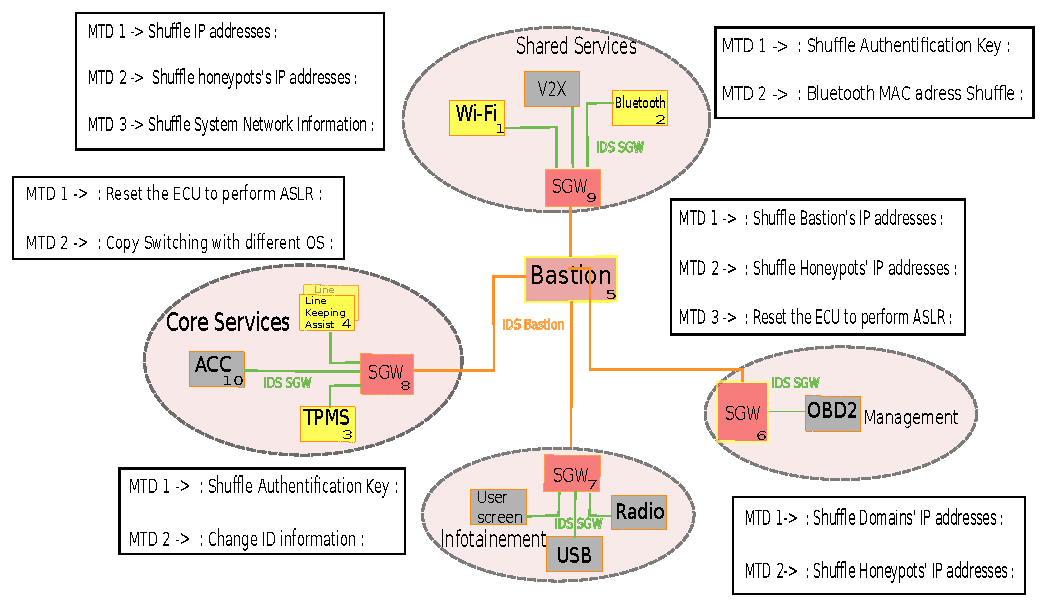
\includegraphics[width=1\textwidth]{schema/archi_comp.pdf}
    \caption{Full game representation}
    \label{fig:archi_mtd}
\end{figure}

This architecture corresponds to a game containing 10 nodes, each having between two and three MTD for defense, with ten attacker profiles taken into account when developing the strategy.
We generated the MILP corresponding to this architecture that we resolved using the CPLEX tool. We obtain the following defense strategy presented in \ref{def_strat} in which the defender will defend each node and MTD targeted by an attacker by spending its budget of 1 per node.  And the attacker strategy presented in \ref{att_strat}.
The time required to compute a solution to the problem with CPLEX is $9.2$ seconds.


\begin{align}
\delta_{n0_m0} &= 0.351 & \delta_{n0_m1} &= 0.0 & \delta_{n0_m2} &= 0.648  & \delta_{n0idl} &= 0.0 \nonumber \\
\delta_{n1_m0} &= 0.95 & \delta_{n1_m1} &= 0.05 & \delta_{n1_m2} &= 0.0 & \delta_{n1idl} &= 0.0 \nonumber  \\
\delta_{n2_m0} &= 0.0 & \delta_{n2_m1} &= 1.0 & \delta_{n2_m2} &= 0.0 & \delta_{n2idl} &= 0.0 \nonumber  \\
\delta_{n3_m0} &= 1.0  & \delta_{n3_m1} &= 0.0 & \delta_{n3_m2} &= 0.0 & \delta_{n3idl} &= 0.0 \nonumber  \\
\delta_{n4_m0} &= 0.403 & \delta_{n4_m1} &= 0.310 & \delta_{n4_m2} &= 0.285 & \delta_{n4idl} &= 0   \nonumber  \\
\delta_{n5_m0} &= 0.0 & \delta_{n5_m1} &= 1.0 &\delta_{n5_m2} &= 0.0 & \delta_{n5idl} &= 0.0  \nonumber  \\
\delta_{n6_m0} &= 0.0 & \delta_{n6_m1} &= 1.0 & \delta_{n6_m2} &= 0.0 & \delta_{n6idl} &= 0 \nonumber  \\
\delta_{n7_m0} &= 0.0 & \delta_{n7_m1} &= 0.921 & \delta_{n7_m2} &= 0.078 & \delta_{n7idl} &= 0  \nonumber  \\
\delta_{n8_m0} &= 0.0 & \delta_{n8_m1} &= 1.0 & \delta_{n8_m2} &= 0.0 & \delta_{n8idl} &= 0 \nonumber  \\
\delta_{n9_m0} &= 0.519 & \delta_{n9_m1} &= 0.480 & \delta_{n9_m2} &= 0.0 & \delta_{n9idl} &= 0 \label{def_strat} \\ \nonumber \\
\alpha_{p0_n0_m0} &= 1.0 & \alpha_{p1_n9_m1} &= 1.0 & \alpha_{p2_n4_m1} &= 1.0 & \alpha_{p3_n1_m0} &= 1.0 & \alpha_{p4_n7_m2} &= 1.0 \nonumber \\
\alpha_{p5_n0_m2} &= 1.0 & \alpha_{p6_n9_m0} &= 1.0 & \alpha_{p7_n4_m0} &= 1.0 & \alpha_{p8_n7_m1} &= 1.0 & \alpha_{p9_n1_m1} &= 1.0  \label{att_strat}
\end{align}


\subsection{Scaling tests}

\subsubsection{Random generator}

In order to investigate if the proposed solution scales well, we have generated random scenarios of different size \footnote{The generating tool we made for the experimentation is available for clone here : https://gitlab.telecom-paris.fr/TheseMA/tool\_for\_journal.git}.

During our experiments, we realized that generating the parameters in a totally random way corresponds to the worst case scenario for the defender in which all the attacker profiles are interested by all the nodes and MTD of the game. This slows down the solution search and limits the size of a game to 15 attacker profiles for 15 nodes. \\

To resolve this issue and to have a more realistic scenario generator, we limit the interest of an attacker to two thirds of the MTD present on the nodes in a random way. 

The results obtained are summarized in Figure~\ref{fig:game_pres}, in which we display the computation time taken by CPLEX to solve the problems. The scenarios are generated in such a way to have as many attacker profiles as nodes. With the parameters of the game generated randomly. This way we get an execution time for a scenario with 10 nodes and 10 attacker profiles of the same range as the one presented in \ref{expe_case}.

\begin{figure}[h]
    \centering
    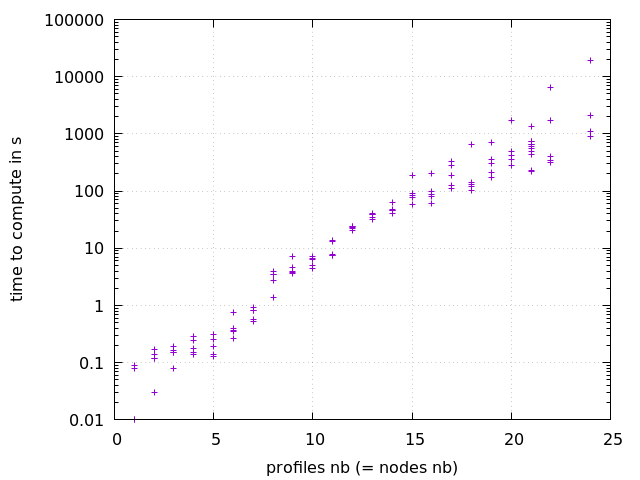
\includegraphics[width=0.75\textwidth]{schema/plot_control_log.png}
    \caption{Scaling representation with attacker profiles number = node number}
    \label{fig:game_pres}
\end{figure}


We manage to reach reasonable times with games composed of 25 nodes and 25 attacker profiles.

An automotive system is made up of an average of a hundred assets that we will try to protect, this amounts to about 25 nodes per domain.

If we consider that the game corresponds to the strategy to be defined on a domain, this is not disadvantageous on the attacker's side, who finds himself attacking each domain once. On the defender's side it does not change anything in the principle of finding the strategy.

\subsubsection{Fixed attacker profiles generator}

In a realistic scenario, it is more common to choose a fixed number of attacker profiles defined in advance according to the type of identified attack scenario being considered.

We can look for the best possible strategy by considering that there will only be privacy attackers interested by the vehicle, and that among these types of attackers, there will be 5 levels of expertise taken into account expert/high/medium/low/beginner. 

If we now consider that we have privacy and integrity attackers targeting the system, with 5 levels of expertise each, we arrive at 10 attacker profiles to take into account in the game.

In the case we want to be even more precise and we know 10 specific attackers trying to attack us in addition to the 10 profiles previously taken into account, we arrive at 20 attacker profiles. \\

We wanted to check up to how many nodes we could consider in order to find a solution, this is represented on the figure~\ref{fig:full}. 
As can be noticed, there are no scenarios where the number of nodes is smaller than the number of attacker profiles considered. This is due to the form of our model in which the attacker has a global budget for the game while the defender has one budget per node. This leads to an infeasibility of the problem because of constraints \ref{c1_milp}, \ref{c3_milp} and \ref{c4_milp} of the MILP. \\

\begin{figure}[h]
    \centering
    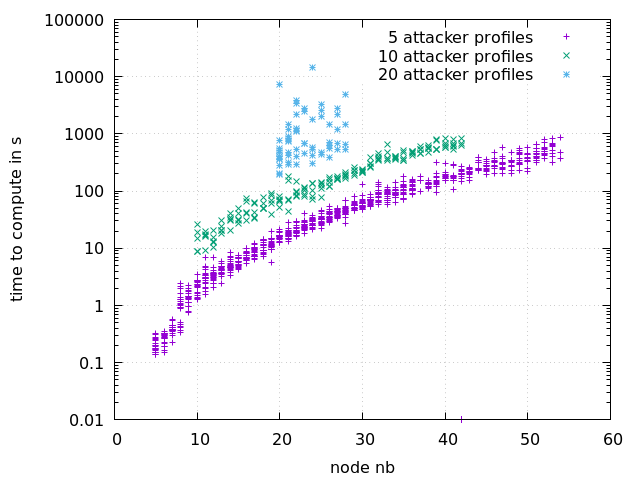
\includegraphics[width=0.75\textwidth]{schema/plot_cplex.png}
    \caption{Scaling representation with fixed attacker number profiles and increasing node number}
    \label{fig:full}
\end{figure}


By looking at the results of the scaling test with different types of attacker profiles considered, we notice that by taking into account 1 type of attacker (5 profiles), it is possible to scale up to 55 nodes with 3 different MTD each. On systems where only one type of attacker is considered, this type of model allows to calculate a strategy for the defender in a reasonable time.

For systems in which 2 types of attackers are taken into account (10 profiles), it is possible to find a solution in a reasonable time for 40 nodes each having 3 MTD. This corresponds to finding a strategy for a domain of a car-like system. 

On the other hand, for systems taking into account a larger number of attacker profiles (20 profiles), we are limited to 30 nodes to find a strategy in a reasonable time. This becomes complicated for automotive systems.

\subsection{Stability Analysis}

We realized a stability analysis on different parameters of our game. As it is difficult to characterize some parameters, we wanted to increase the confidence we have in our model in case of an approximation error in the definition of some parameters such as the rate of appearance of an attacker profile, or the cost of an attack for an attacker. \\

We therefore started with the parameter $\gamma$ representing the rate of appearance of an attacker profile. We then varied the ratio between the two types of attackers (privacy and integrity) for a lambda configuration of their exponential distribution in order to see the impact that this would have on the defender's strategy. We started with a configuration of the game similar to the one presented in the example case, 10 nodes each having between 2 and 3 MTD being targeted by 10 attacker profiles.
The results of this experiment for 4 of the nodes in our game are presented in figure \ref{fig:gamma}. \\

\begin{figure}[h]
    \centering
    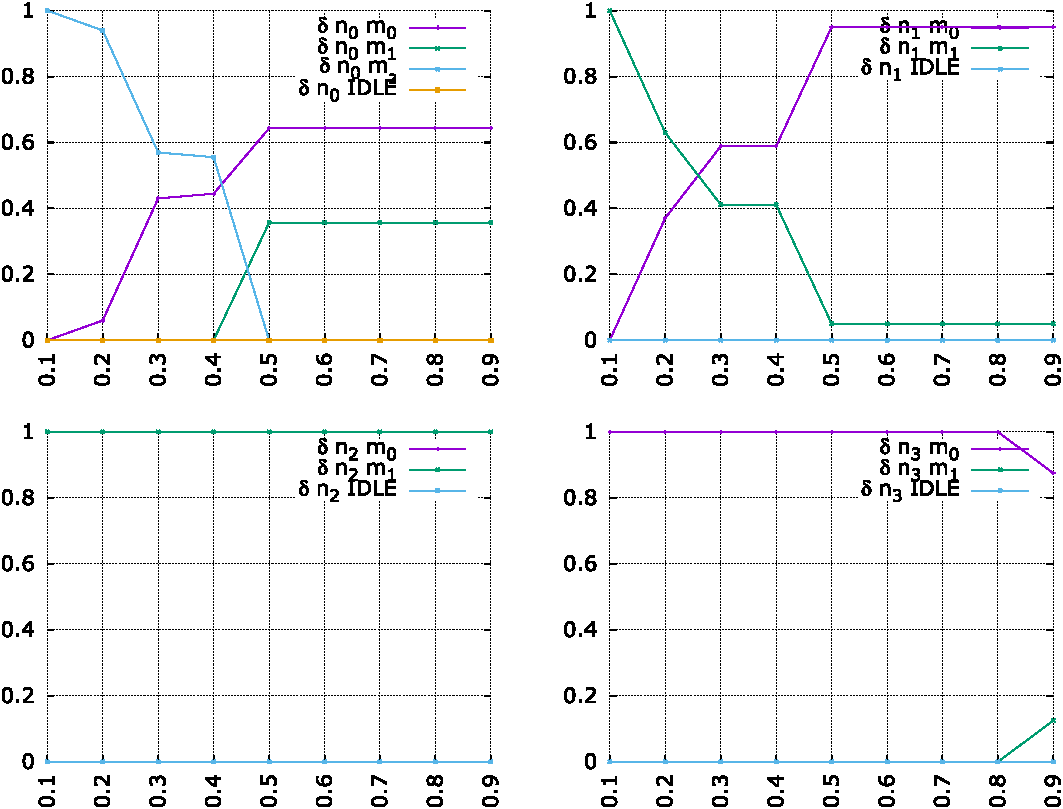
\includegraphics[width=1\textwidth]{schema/multiplot_gamma.pdf}
    \caption{How moving the ratio between attacker profiles (gamma) affect the defender strategy}
    \label{fig:gamma}
\end{figure}


We notice that the variation is linear, and that the defender's strategy reacts in a normal way to the change of ratio between the attackers.
On a node like number 0 and 1 on which more attacker profiles target them, depending on the ratio of attacker profile, the strategy evolves in order to defend more efficiently against the type of attacker becoming more present.

On nodes such as node number 2, targeted by no attacker type, this does not change the strategy of the defender, and on the fourth node, when the ratio of the second attacker type becomes more present, the strategy of the defender starts to adapt. \\


In order to then look at the stability of the given strategy according to a set of input parameters, we sum of a fixed scenario using the configuration of the example case. Then we randomly shuffled the value of the costs and gain for the defender and the attacker as well as the attacker success value of the scenario around a certain percentage of variance in order to check the stability of the output strategy. The result of this variance is represented in figure \ref{fig:multiplot} with box plot representing the variation of strategy of the defender on 100 different scenario. 

\begin{figure}[h]
    \centering
    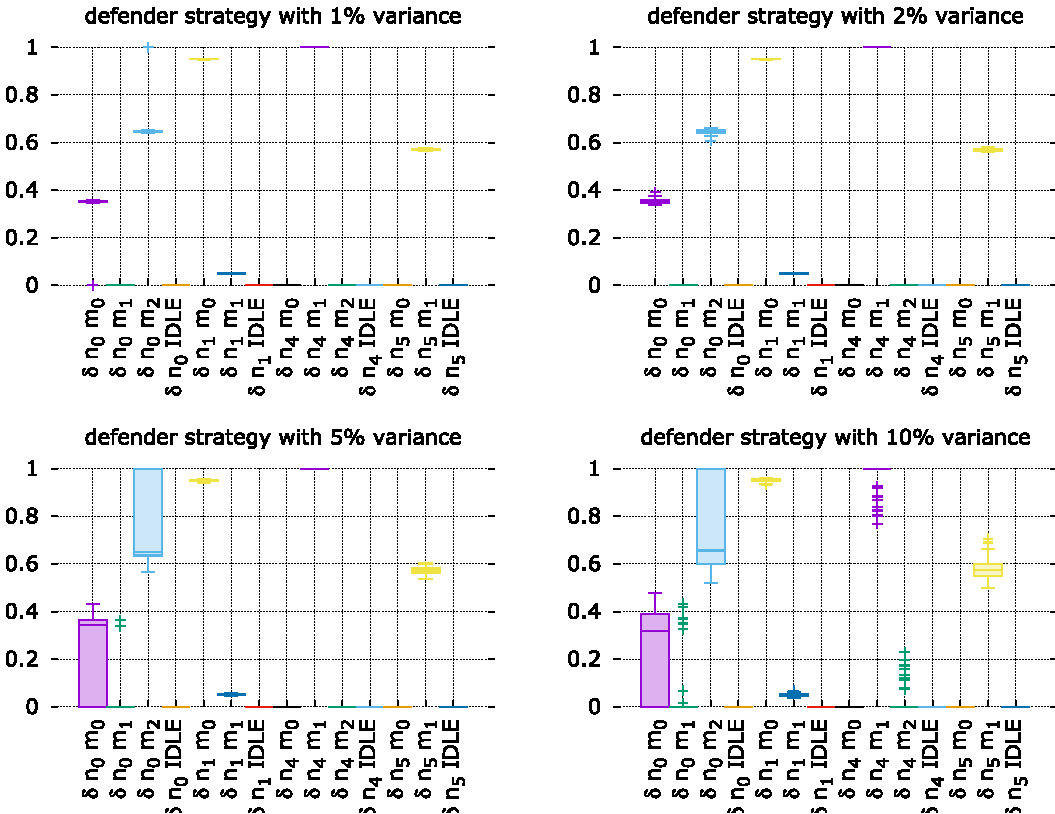
\includegraphics[width=1.0\textwidth]{schema/multiplot.pdf}
    \caption{How stable the strategies are considering variance in the parameters}
    \label{fig:multiplot}
\end{figure}

We also notice that the strategy variation remains quite stable up to 5\%. At this moment, on the node 0 where the balance between the two attackers is borderline, we notice a change of strategy. But we notice that the medians of the strategies on this node are still located in the same order of magnitude, indicating that the strategy remains mostly located in the same area.
From 10\% we start to notice a more important variance in the strategy of the defender, with an average strategy always located in the same region.
We can say that our model reacts in a normal way to the variations in the parameters and is quite stable allowing us to have confidence in the final strategy taking into account a small possible margin of error in the definition of the parameters.


\chapter{Conclusions et perspectives} \label{CONCL} \smallskip \hfill
\begin{minipage}[b]{8cm}
{\it Je vois refl\'eter dans mon miroir tout mon pass\'e et tout mon avenir.}
\end{minipage}
\begin{flushright} J. Cort\'azar. \end{flushright}
\bigskip

%\section{Les le\c cons apprises}

%Aucune !
\bigskip

\section{Les fronti\`eres de la recherche}

The sky is the limit...


% Acronyms and gloaasry
\clearpage
\printglossary[type=\acronymtype]

\printglossary

\newpage
\printbibliography

\newpage
\appendix
\chapter{Ma belle annexe} \label{ANNEXE_1}

\section{Introduction}

La th\'eorie....  \medskip

Ceci est une appendice...


\end{document}
